% MSc dissertation example file, February 2022
%
% Leave one of the documentclass lines uncommented to match your degree.
% You may remove the logo option if it causes problems.
% Do not change any other options.
% \documentclass[logo,msc,adi]{infthesis}     % Adv Design Inf
% \documentclass[logo,msc,ai]{infthesis}      % AI
% \documentclass[logo,msc,cogsci]{infthesis}  % Cognitive Sci
% \documentclass[logo,msc,cs]{infthesis}      % Computer Sci
% \documentclass[logo,msc,cyber]{infthesis}   % Cyber Sec
% \documentclass[logo,msc,datasci]{infthesis} % Data Sci
% \documentclass[logo,msc,di]{infthesis}      % Design Inf
% \documentclass[logo,msc,dsti]{infthesis}    % Data Sci TI
% \documentclass[logo,msc,inf]{infthesis}     % Informatics
\documentclass[logo,msc]{infthesis}           % degree unspecified, do not change except to add your degree
%%%%%%%%%%%%%%%%%%%%%%%%
% Understand any problems and seek approval before assuming it's ok to remove ugcheck.
\usepackage{msccheck}

% Include any packages you need below, but don't include any that change the page
% layout or style of the dissertation. By including the ugcheck package above,
% you should catch most accidental changes of page layout though.

\usepackage{microtype} % recommended, but you can remove if it causes problems

% MY PACKAGES 
\usepackage{algorithm}
\usepackage{algpseudocode}
\usepackage{amsmath}
\usepackage{xcolor}
\usepackage{tikz}
\usetikzlibrary{shapes,arrows,positioning,fit,backgrounds}
%\usepackage[most]{tcolorbox} % Load tcolorbox with most libraries
\usepackage{tcolorbox}
\usepackage{amsmath} % For math symbols and align environment
\usepackage{booktabs}
\usepackage{graphicx}
\usepackage{array}
\usepackage{longtable} % Allows tables to span multiple pages if needed
\usepackage{listings} % Include the listings package for formatted code blocks
\usepackage{xcolor} % For colored text
\usepackage{geometry}
\usepackage{svg}
\usepackage{pgfplots}
\usepackage{pgfplotstable}
\pgfplotsset{compat=1.18}
\usepackage[hidelinks]{hyperref}
\tcbuselibrary{skins} % Load other necessary libraries
\pgfplotsset{width=7cm,compat=1.17}



% ends here packages
\begin{document}
\begin{preliminary}

\title{Large language model number handling in the Finance Domain}

\author{Anant Raj}

\date{\today}

\abstract{
% This skeleton demonstrates how to use the \texttt{infthesis} style for
% MSc dissertations in the School of Informatics. It also emphasises the
% page limit and associated style restrictions for Informatics dissertations
% with course code \texttt{INFR11077}. If your degree has a different project
% course code, then it is likely to have different formatting rules.
% The file \texttt{skeleton.tex} generates this document and should be used as a
% starting point for your thesis. Replace this abstract text with a concise
% summary of your report.
The integration of large language models (LLMs) in the financial domain requires scrupulous attention to numerical precision and the ability to process diverse data types. In this study, we enhance the capabilities of open-source Llama models through an innovative fine-tuning approach that leverages a hybrid dataset, combining tabular data, conversational histories, and contextual information. We employ specialized prompting, few-shot learning, and Chain of Thought reasoning to address complex numerical tasks inherent to financial analysis. Furthermore, we guide the models to generate Python scripts aimed at bolstering numerical accuracy. Our approach offers valuable insights into the potential and challenges of LLMs in complex numerical reasoning within financial contexts, illuminating areas for further enhancement. Our findings highlight the ongoing difficulties in merging varied data forms within LLM frameworks and underscore the necessity for continued refinement of these models to meet the rigorous demands of financial data analysis. This research not only advances our understanding of LLM applications in finance but also sets a foundational framework for future explorations aimed at enhancing the robustness and precision of financial data processing.
}

\maketitle

\newenvironment{ethics}
   {\begin{frontenv}{Research Ethics Approval}{\LARGE}}
   {\end{frontenv}\newpage}

\begin{ethics}
% \textbf{Instructions:} \emph{Agree with your supervisor which
% statement you need to include. Then delete the statement that you are not using,
% and the instructions in italics.\\
% \textbf{Either complete and include this statement:}}\\ % DELETE THESE INSTRUCTIONS
% %
% % IF ETHICS APPROVAL WAS REQUIRED:
% This project obtained approval from the Informatics Research Ethics committee.\\
% Ethics application number: ???\\
% Date when approval was obtained: YYYY-MM-DD\\
% %
% \emph{[If the project required human participants, edit as appropriate, otherwise delete:]}\\ % DELETE THIS LINE
% The participants' information sheet and a consent form are included in the appendix.\\
%
% IF ETHICS APPROVAL WAS NOT REQUIRED:
% \textbf{\emph{Or include this statement:}}\\ % DELETE THIS LINE
This project was planned in accordance with the Informatics Research
Ethics policy. It did not involve any aspects that required approval
from the Informatics Research Ethics committee.

\standarddeclaration
\end{ethics}


\begin{acknowledgements}
% Any acknowledgements go here.
Embarking on this thesis journey has been an exhilarating experience, and I am profoundly grateful to those whose support has been indispensable. My heartfelt thanks to Professor \textit{Alexandra Birch}, whose unwavering commitment and insightful guidance have been cornerstones of my research. Her scholarly rigor and the access she facilitated to the Valhalla server and the statmt slack community were pivotal during critical phases of my work. Special thanks to \textit{Mateusz}, whose innovative ideas significantly streamlined my research process. Additionally, I owe a tremendous debt of gratitude to my sister, \textit{Priya}, whose boundless patience and encouragement, especially across challenging time zones, have been invaluable. Her willingness to listen and her unyielding presence have been my comfort and strength. This dissertation is not just a product of my individual effort but a testament to the collective support of everyone who cheered me on. Thank you all for being part of my journey.

\begin{comment}
    

Embarking on this thesis journey has been an exhilarating experience, marked by challenges and triumphs alike. As I reflect on this pivotal chapter of my academic career, I am profoundly grateful to a remarkable group of individuals whose support has been indispensable.

Firstly, I extend my heartfelt thanks to my supervisor, Professor \textit{Alexandra Birch}, whose unwavering commitment and insightful guidance have been cornerstones of my research endeavor. She has not only enriched our discussions with her profound expertise but has also adeptly navigated me through the complexities of experimental analysis. Her patience and scholarly rigor have greatly enhanced my work, and I am especially grateful for her facilitating access to the Valhalla server and introducing me to the invaluable statmt slack community, whose support was pivotal during critical phases of my research.

A special acknowledgment to \textit{Mateusz}, whose morale-boosting encouragement was a beacon during moments of doubt. Similarly, \textit{Patrick’s} introduction of innovative ideas has significantly streamlined my research process, for which I am immensely thankful.

I am also blessed with an incredible support system of friends and family whose belief in my potential has been a constant source of strength. Your unwavering support and love have been fundamental to my perseverance and success.

And \textit{Priya}, my sister – you deserve a special mention. You've been my rock throughout this whole dissertation madness and beyond. Thanks for listening to me ramble on and on, complain about everything under the sun, and still being there for me despite the crazy time differences. You're the best.

This dissertation is not solely a product of my individual effort but a testament to the collective support and encouragement of everyone mentioned, and to those unnamed who cheered me from the sidelines. To all of you, I offer my deepest appreciation and gratitude. Thank you for being part of my journey.
\end{comment}
\end{acknowledgements}


\tableofcontents
\end{preliminary}


\chapter{Introduction}

The intersection of Large Language Models (LLMs) and the financial industry represents a promising yet challenging frontier. LLMs such as GPT-4 and Claude AI have demonstrated significant capabilities across various Natural Language Processing (NLP) tasks, driven by advanced training methods like reinforcement learning from human feedback (RLHF) and masked language modeling \cite{li2023chatgpt}. However, these models also have notable limitations, including difficulties with current information access, arithmetic tasks, and a tendency to generate inaccurate responses due to hallucinations \cite{schick2023toolformer,li2024dawn}. Despite being trained on diverse datasets, their performance in specialized domains like finance remains underexplored.
LLMs are increasingly integral to financial applications such as investment sentiment analysis, named entity recognition, question-answering, and stock market prediction. These tools assist analysts in managing complex datasets and predictive models. Methods like multi-field LLMs and instruction fine-tuning have been explored to improve results in financial contexts \cite{lee2024survey}. However, the nuanced understanding and processing of complex financial data by LLMs are still in early stages, necessitating further empirical study.

%This project aims to investigate various number-handling strategies to fine-tune a large language model using instruction data, with the goal of achieving optimal performance in finance-related downstream tasks, particularly those involving currency or numerical questions. 
%This research endeavor seeks to systematically explore multiple fine-tuning methodologies applied to open-source language models, incorporating instruction tuning, few-shot prompting, and chain-of-thought reasoning. In prior works, all these techniques have been studied and applied on different datasets across domains. Jason et al. (2022) has noted that instruction tuning language models on tasks that are naturally articulated as instructions, like translation, question-answering and reading comprehensions substantially improves zero shot performance on unseen tasks \cite{wei2022finetunedlanguagemodelszeroshot}. Kojima et al. (2023) came out with the idea of zero-shot CoT that essentially involves adding "Let's think step by step" to the original prompt. Their experiments yeilded impressive results using single prompt template on diverse reasoning tasks including arithmetic, symbolic reasoning and logical reasoning tasks \cite{kojima2023largelanguagemodelszeroshot}. Brown et al. (2020) demonstrated the in context learning where examples are provided in the prompt to steer the model to better performance. The number of examples to be chosen depends on the complexity of the task. 
%For this research work our objective is to enhance model performance on finance-specific downstream tasks that necessitate numerical computation and complex reasoning within financial contexts. A diverse set of 4 financial datasets has been selected, encompassing tabular data, contextual information, relation extraction, and Conversational Finance Question Answering. These complex numerical reasoning datasets provide a robust foundation for generalizing across a wide range of financial tasks. The choice of these dataset poses a unique challenge which has not been addressed or experimented in previous works - due to the diversity of the datasets there's no one shoe fit all approach that can be used here. For eg. it is a limitation of Few Shot Prompting (FSP) that it works well for many tasks but is still not a perfect technique, especially when dealing with more complex reasoning tasks which is 3 out o f the 4 dataset in our case namely TAT-QA, ConvFinQA and FinQA. All these datasets have diverse mix of samples and requires high level of understanding of reasoning tasks coupled with arithmetic solving capability and precise extraction of tabular data. To add to the complexity is the relation extraction dataset which requires extracting the most prominent relation from given input. It adds the generalisation required to build the model robust for general usage. Using instruction tuning has the challenges to create high-quality instructions for use in fine-tuning. If we look at the examples detailed in section [add reference - A.2], it is worth noting that even in one of the dataset for instance TAT-QA it posses different level of challenges - in the first example only extraction of data from table is sufficient to generate the response while in the second example the model has to perform some calculation post extraction of the data to come up with the final answer. Similarly for ConvFinQA, the challenges lies in understanding the textual and tabular data from the input and then understand (and also note in some way) the question answer history of the conversation to finally answer the question [add reference -A.2 example]. Also to be noted is the variable length of the input in these datasets where the ConvFinQA input length is very long and it requires the input token to be in full and not truncated else it won't be able to see the final question and hence will not be able to generate correct response. We identified these challenges and experimented with standard fine tuning approach first, Initially, baseline performance was assessed on open-source models such as Llama2 and the newly launched Llama3 using these datasets. It is well known that large language models (LLMs) often struggle with numerical data, particularly in tasks requiring numerical reasoning, and our results were consistent with this observation. Several fine-tuning approaches were explored, starting with the Llama2-chat 7B model and subsequently extending experiments to the latest Llama3 8B models. Recognizing that a single technique does not suffice for all scenarios due to the challenges we discussed and the diversification in the dataset, various techniques were experimented with from FSP to CoT and instruction tuning. After rigorous experiments we came to the conclusion that the mixture of - FSP and CoT is the most efficient way to deal with the discussed challenges encompassing all the variances in the curated dataset. This is a novel approach in financial domain although prior works like that of Kim et al.(2023) demonstrated improvement in zero shot and few shot via Chain-of-Thought Fine tuning on BIG-Bench-Hard (BBH) benchmark and domain specific tasks \cite{kim2023cotcollectionimprovingzeroshot}. Zhu et al. (2024) utilised the step-wise pipeline approach for tabular and textula QA for better multi-step inference using extractor, reasoner and executor by fine tuning Llama2 models on TAT-QA, FinQA and TAT-DQA datasets but it is different from our work in a significant way - we didn't solely focused on tabular and textual samples, we have conversational QA and relation extraction dataset which are more generalised since financial domain is not limited to just tabular and textual data. Also they reported the model facing challenges in precisely interpreting the meaning of the values due to the use of external executor and since we don't rely on external tools in fine tuning and just rely on models input to generate responses. 
\begin{figure}[h]
    \centering
    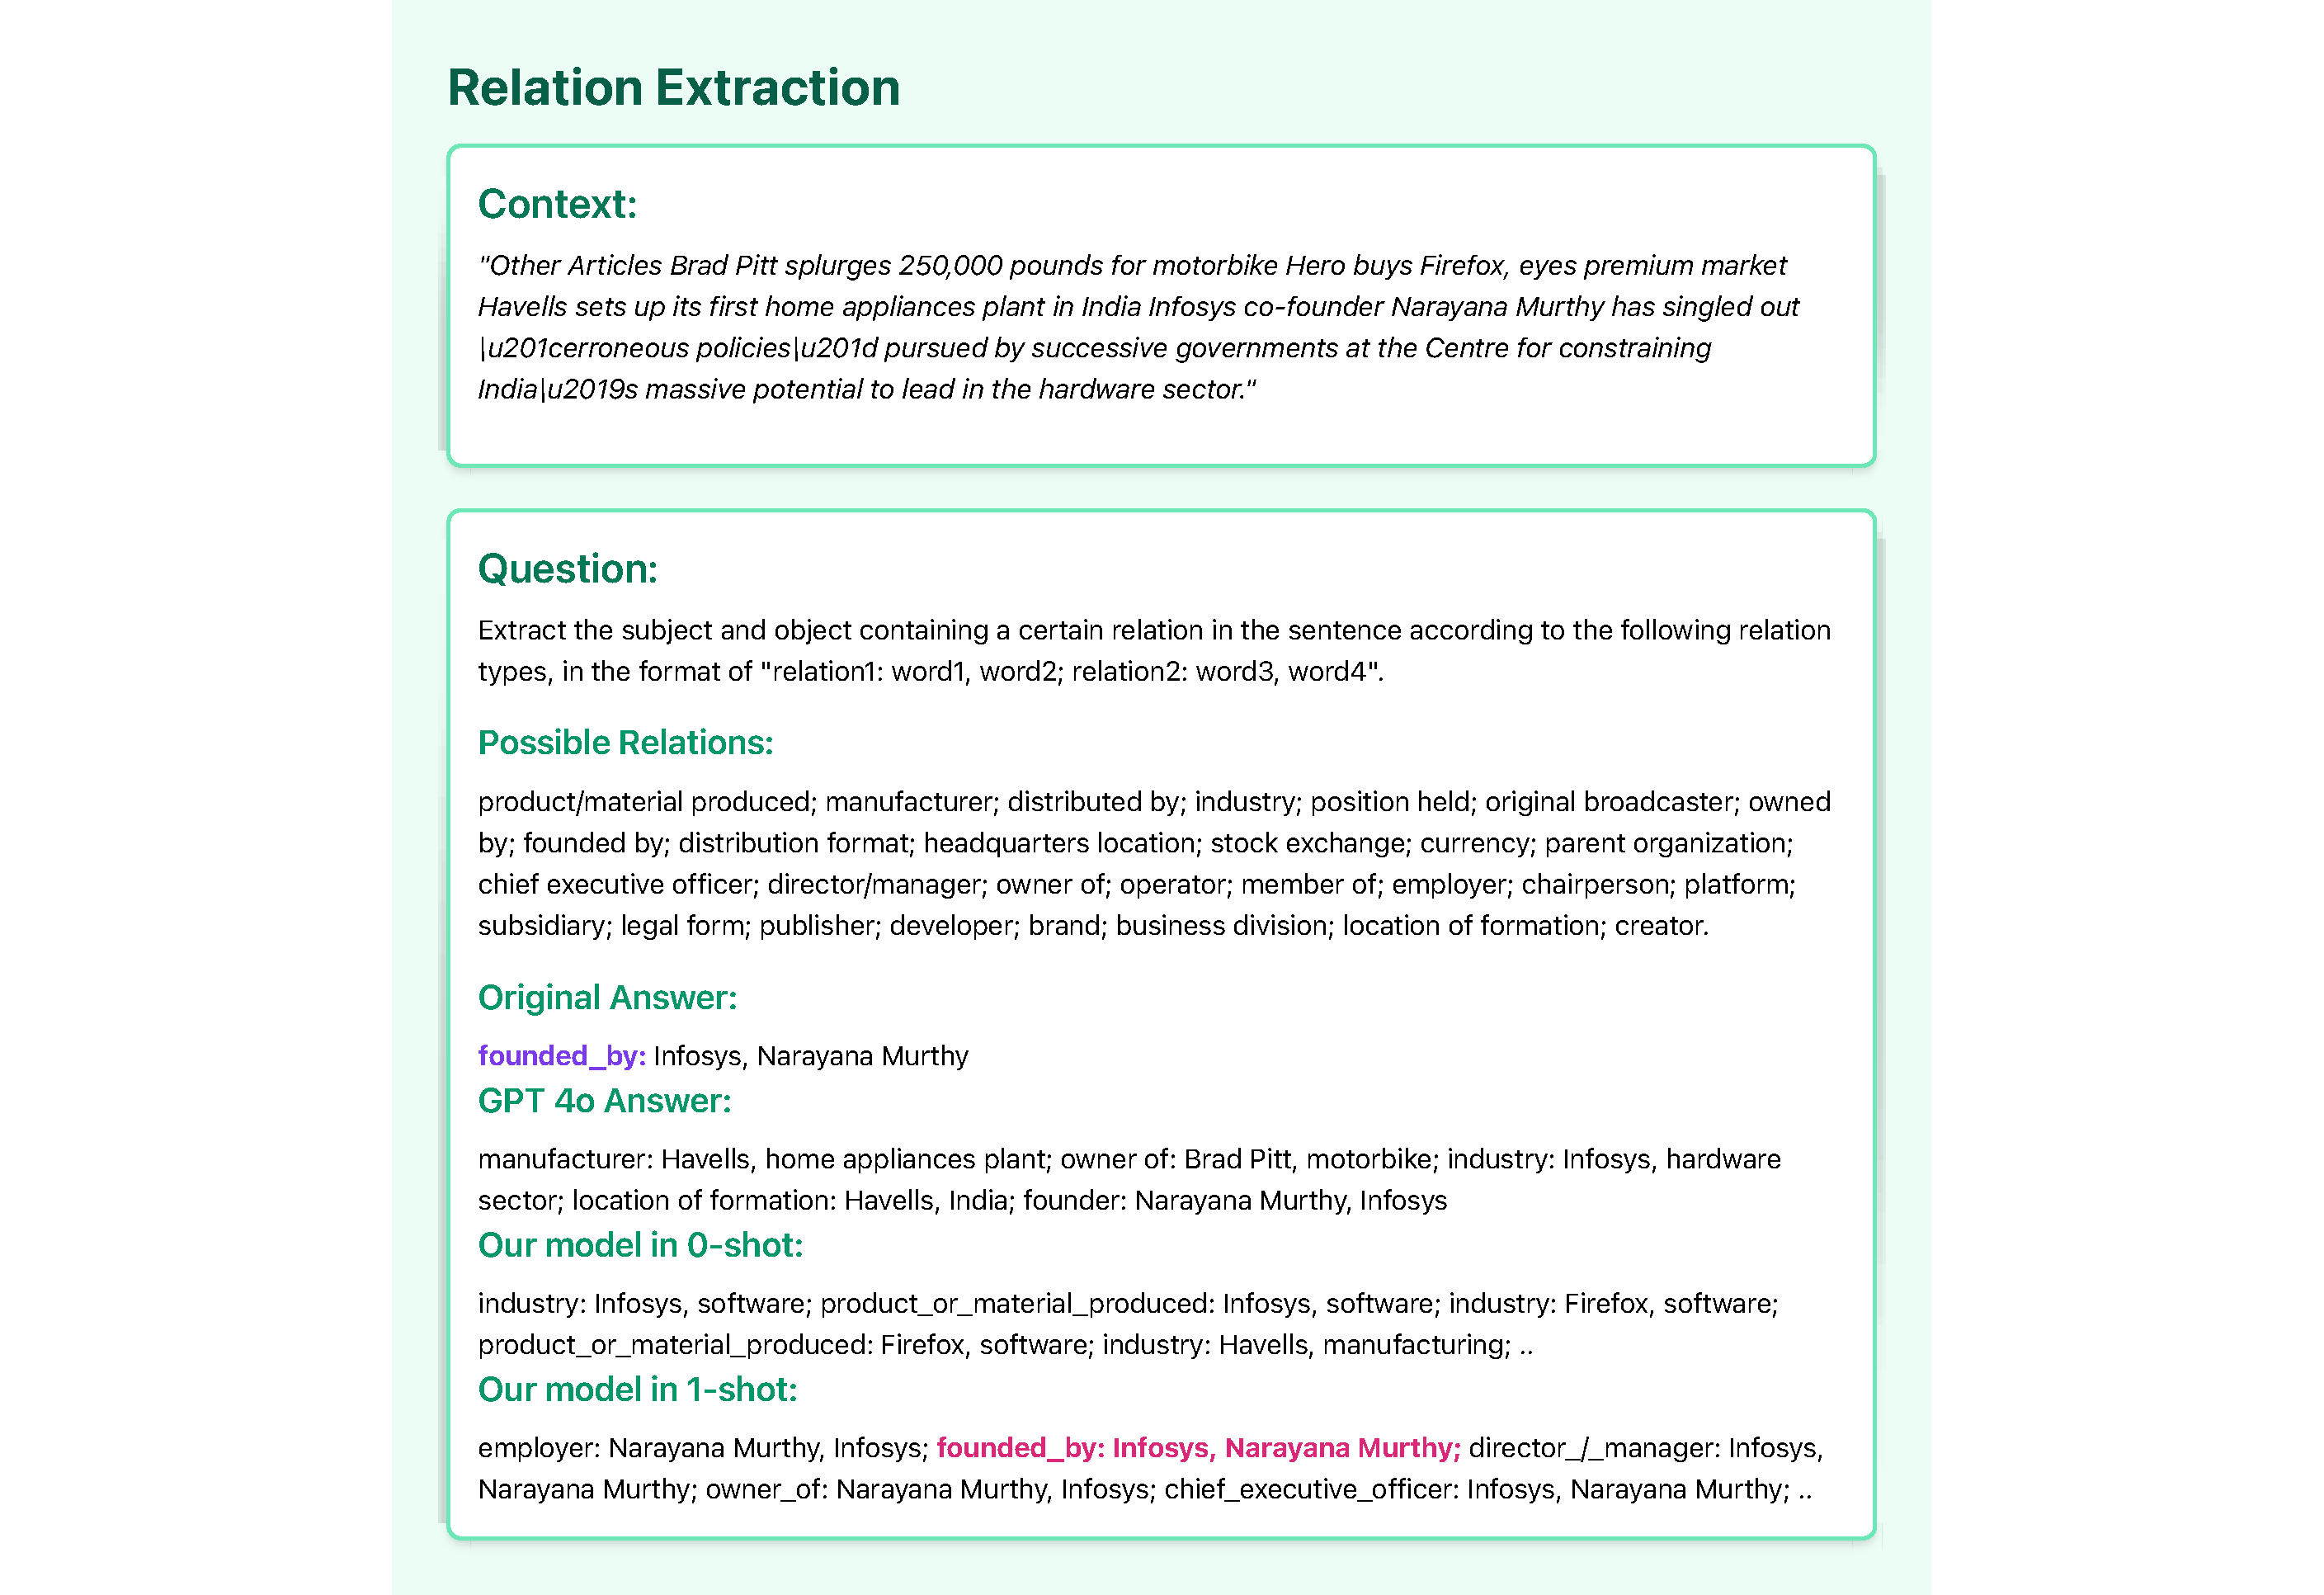
\includegraphics[width=0.8\textwidth, height=0.7\textheight, keepaspectratio]{mscdiss-skeleton/relext_updated.pdf}
    \caption{Relation extraction sample with GPT-4o and our model in 0-shot and 1-shot.}
    \label{relext}
\end{figure}


This research investigates various fine-tuning methodologies for open-source language models, focusing on instruction tuning, few-shot prompting, and chain-of-thought reasoning. Previous studies have demonstrated that these techniques can enhance performance across diverse tasks, including translation, question-answering, and complex reasoning \cite{wei2022finetunedlanguagemodelszeroshot,kojima2023largelanguagemodelszeroshot,brown2020language}. Our study aims to apply these methods to finance-specific tasks that require numerical computation and complex reasoning. We utilize four diverse financial datasets, which include tabular data, contextual information, relation extraction, and conversational finance question-answering, to challenge the models and enhance generalizability across various financial tasks. The diversity of the datasets poses a unique challenge, as there is no one-size-fits-all approach that can be applied effectively. For example, few-shot prompting (FSP) performs well on many tasks but may struggle with more complex reasoning tasks, which constitute three out of the four datasets in this study (TAT-QA, ConvFinQA, and FinQA). These datasets require a high level of reasoning, arithmetic solving capability, and precise extraction of tabular data. The relation extraction dataset further adds the generalization required to build a robust model for general usage. Figure~\ref{relext} illustrates the performance of the latest GPT-4o model in relation extraction tasks. Despite its advancements, GPT-4o often generates multiple extractions per query, whereas the reference contains only one. Conversely, our model in one-shot, produces the correct extraction but also includes additional extractions. This issue stems from the dataset's ambiguity regarding the acceptable number of responses, allowing multiple relevant extractions as per the context and question. In relation extraction, the significance of input tokens varies. However, standard prompt templates for classification treat all words equally, failing to reflect this differential importance effectively \cite{liu2021pretrainpromptpredictsystematic}. Additionally, the challenge of instruction tuning arises, necessitating the creation of high-quality instructions for fine-tuning to address the complexities introduced by variations across different datasets. Even within a single dataset, such as TAT-QA, the level of difficulty varies, with some examples requiring only data extraction from tables (for sample~\ref{tat-qa-app}), while others necessitate additional calculations to generate the final answer. Similarly, for ConvFinQA, the challenges lie in understanding the textual and tabular data from the input and keeping track of the question-answer history of the conversation to provide the correct response(see Figure~\ref{convfin}). Furthermore, the variable length of the input, with ConvFinQA having particularly long inputs, requires the model to process the full context without truncation to generate accurate responses.
\begin{figure}[h]
    \centering
    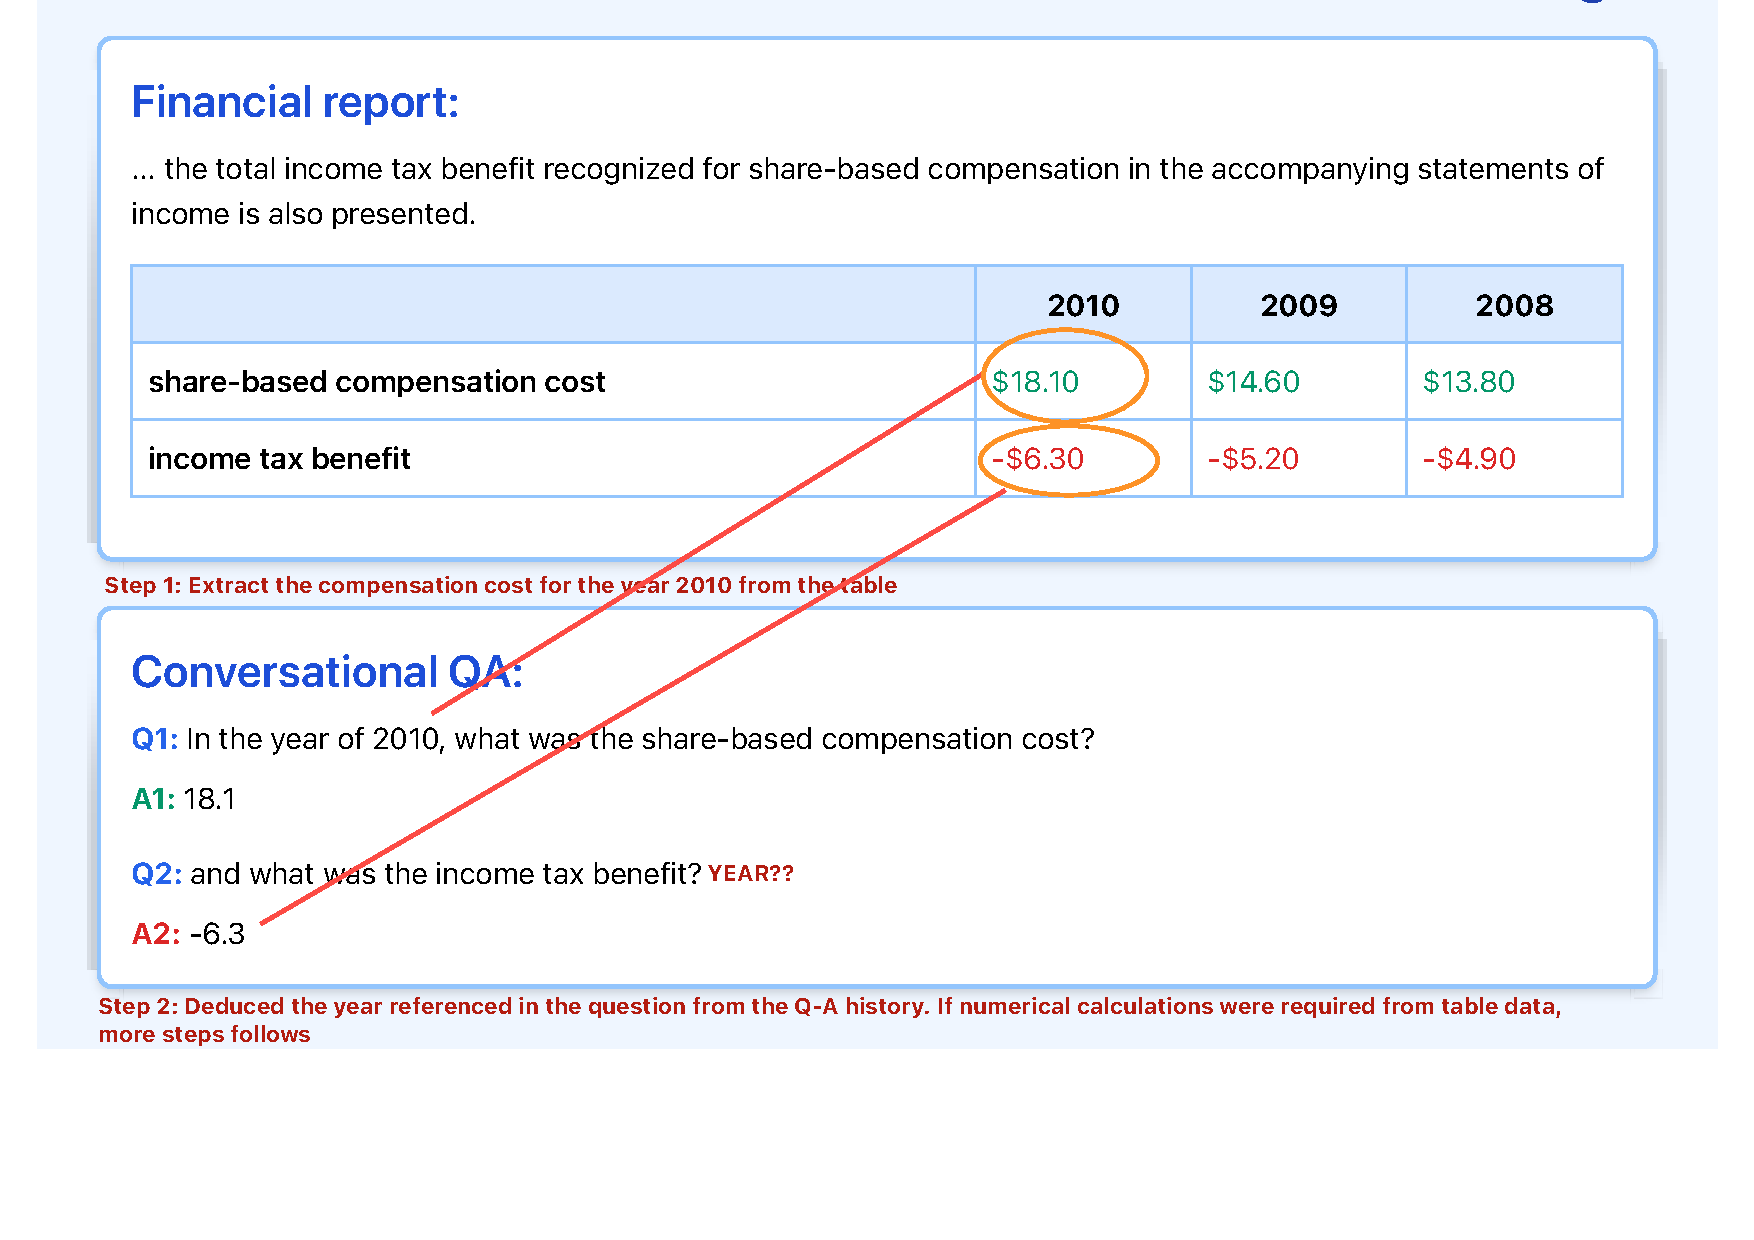
\includegraphics[width=0.70\textwidth]{mscdiss-skeleton/ConvFinQa_scaled.pdf}  
    \caption{QA History in ConvFinQA}
    \label{convfin}

\end{figure}

Initial experiments with open-source models like LLaMA2 and LLaMA3 confirmed that LLMs often struggle with numerical reasoning, relation extraction and hybrid tasks. Various fine-tuning approaches, including FSP, chain-of-thought (CoT), and instruction tuning, were explored. Ultimately, a combination of FSP and CoT proved most effective in addressing the dataset's challenges. This approach, particularly novel in the financial domain, builds on previous works \cite{kim2023cotcollectionimprovingzeroshot,zhu2024tatllmspecializedlanguagemodel} but extends their scope to include conversational question-answering and relation extraction tasks, further enhancing the model's robustness and generalizability.

%The study initially assessed baseline performance on open-source models such as LLaMA2 and the newly launched LLaMA3, consistent with the observation that large language models (LLMs) often struggle with numerical data, particularly in tasks requiring numerical reasoning. Several fine-tuning approaches were explored, starting with the LLaMA2-chat 7B model and subsequently extending experiments to the latest LLaMA3 8B models. Recognizing that a single technique does not suffice for all scenarios due to the challenges and dataset diversification, various techniques were experimented with, including FSP, chain-of-thought (CoT), and instruction tuning. After rigorous experiments, we concluded that a mixture of FSP and CoT is the most efficient approach to address the challenges posed by the curated dataset. This novel approach in the financial domain builds upon prior works, such as Kim et al. (2023), which demonstrated improvements in zero-shot and few-shot performance via chain-of-thought fine-tuning on the BIG-Bench-Hard (BBH) benchmark and domain-specific tasks \cite{kim2023cotcollectionimprovingzeroshot}. Additionally, Zhu et al. (2024) utilized a step-wise pipeline approach for tabular and textual question-answering, fine-tuning LLaMA2 models on TAT-QA, FinQA, and TAT-DQA datasets \cite{zhu2024tatllmspecializedlanguagemodel}. However, the present study differs from Zhu et al.'s work in a significant way, as it not only focuses on tabular and textual samples but also includes conversational question-answering and relation extraction datasets, which are more generalized, as the financial domain is not limited to just tabular and textual data. Furthermore, the present study does not rely on external tools for precise interpretation of values, as reported by Zhu et al., but rather leverages the model's own input-to-output generation capabilities, utilizing fine-tuning and the other approaches mentioned above. 
%[Mention percentage increase improvement in the best model]

In our next study, we extend the innovative principles of Schick et al. (2023) from their seminal work \textit{Toolformer: Language Models Can Teach Themselves to Use Tools}, which demonstrated the enhancement of language models' performance by integrating external tools like calculators and search engines \cite{schick2023toolformer}. Inspired by this, our study introduces a sophisticated pipeline that integrates LangChain agents and function calling to address the challenges posed by complex datasets like TAT-QA. This approach employs a combination of few-shot prompting (FSP), instruction tuning, and Chain of Thought (CoT) reasoning. By leveraging these strategies, our methodology enables language models to independently generate and execute Python code, thus significantly enhancing their reasoning and computational capabilities for complex financial tasks.

The pilot study utilized the \textsc{facebook/opt-1.3b} model in conjunction with LangChain's Python agent to produce promising results. This was further scaled to the more powerful Llama-3.1-8b-instruct model, handling more complex datasets like TAT-QA. These experiments underscore the pivotal role of model size and computational power in processing demanding financial datasets effectively.

Our research not only advances the capabilities of language models in financial applications but also discusses critical aspects of scalability and the balance between computational power and model sophistication. Our findings suggest that with strategic implementation of code generation pipeline, LLMs can achieve state-of-the-art performance in financial tasks, paving the way for future advancements in the use of open-source models for financial analysis. 

%we venture beyond the traditional confines of fine tuning language models on downstream tasks, drawing upon the groundbreaking work of Schick et al. (2023) who demonstrated the potent use of external tools by LLMs in their paper \textit{Toolformer: Language Models Can Teach Themselves to Use Tools}. This paper showed how integrating functionalities like calculators, Q&A systems, and search engines could significantly enhance a model's performance with numerical data \cite{schick2023toolformer}. Our study expands on this concept by incorporating LangChain agents and function calling to leverage external computational tools, aiming to bridge the gap between LLM capabilities and the intricate demands of financial data analysis. Our approach revolves around the hypothesis that by employing a few-shot prompting (FSP) strategy combined with instruction tuning and Chain of Thought (CoT) reasoning, LLMs can be directed to generate code that interacts with external tools, enhancing their performance in financial applications. This strategy is informed by the observation that step-by-step problem-solving — akin to how a human would approach a reasoning task — is an effective method for tackling complex questions. For example, in estimating the impact of macroeconomic changes on stock prices, the model would first identify relevant economic indicators, calculate their changes over time, and then analyze the correlation with stock market trends, before generating a comprehensive report.

%Our innovative pipeline approach employs this CoT methodology to structure the generation of Python scripts, which are then executed using Python’s \textit{exec} function. This allows the model to harness Python’s extensive computational abilities directly, thereby enhancing its capability to perform complex calculations and analyses typically required in the financial sector.

%In our pilot study, we initially applied this technique using the smaller \textsc{facebook/opt-1.3b} model, combined with LangChain's Python agent, to achieve promising results. Subsequently, we scaled this approach to the more robust Llama-3.1-8b-instruct model for more demanding datasets like TAT-QA. Although scaling up introduced complexities, the outcomes were compelling, highlighting the importance of model size and computational power in achieving high accuracy and reliability in financial analyses.

%By not relying on the inherent code generation capabilities of LLMs but instead directing them through structured CoT reasoning and external computational tools, our research demonstrates a significant improvement in handling complex financial datasets. This methodical enhancement in code generation not only contributes to the field of NLP and financial analytics but also raises important considerations about the scalability of LLMs in practical financial applications and the balance needed between computational efficiency and model sophistication.

%Our findings suggest that with strategic implementation, LLMs can achieve state-of-the-art performance in financial tasks, paving the way for future advancements in the use of open-source models for sophisticated financial analysis. 

\begin{comment}
In our next study, we venture beyond the traditional confines of fine tuning language models on downstream tasks, drawing upon the groundbreaking work of Schick et al. (2023) in their paper \textit{Toolformer: Language Models Can Teach Themselves to Use Tools} where they utilized external tools like a calculator, a Q\&A system, two different search engines, a translation system, and a calendar to elevate the performance of models handling numerical values over those processing textual data and achieved impressive results in zero-shot performance across a variety of downstream tasks \cite{schick2023toolformer}. This approach aligns with cutting-edge developments in recent times like LangChain agents and function calling, which empower models to leverage external capabilities effectively.

Our research work explores the potential of LLMs in processing and analyzing intricate financial datasets, addressing the current limitations in computational power and the scarcity of open-source models capable of handling extensive contextual inputs typical of financial data. Our study operates under the hypothesis that, with optimal resource allocation and fine-tuning using FSP, LLMs can significantly enhance their script generation capabilities, potentially surpassing existing benchmarks in numerical accuracy and analytical depth. This innovative approach is informed by the mechanisms of code generation in reasoning tasks, which involve decomposing the problem into steps, akin to the Chain of Thought (CoT) approach, and then utilizing available libraries for computation. This is posited to be more effective than relying on the LLMs' inherent calculation capabilities, as it can leverage external tools like Python's REPL or the \textit{exec} function, thus utilizing Python's robust computational abilities. To investigate this hypothesis, we conducted a two-phase pilot study. Initially, we utilized a compact, curated dataset sample with the relatively small \textsc{facebook/opt-1.3b} model, integrated with LangChain's Python agent (\textit{python\_repl}), which yielded promising preliminary results. Building on this success, we expanded our experiment, employing the larger Llama-3.1-8b-instruct model to generate Python scripts for more extensive financial datasets, specifically the TAT-QA dataset, executed through Python's \textit{exec \footnote{https://docs.python.org/3/library/functions.html#exec}} function in a structured pipeline. While this larger-scale experiment did not achieve the same level of precision as the initial, smaller sample, it produced compelling outcomes that underscore the critical role of model size and sophistication in code generation for complex inputs, highlighting that generating code with inputs as intricate as the TAT-QA dataset poses substantial challenges for a model of the 8b scale.

Our experiment sought to validate the prevailing belief that larger models with specialized fine-tuning enhance performance, particularly in the domain of code generation for financial analysis. The study demonstrated that reducing error rates in code generation significantly influences accuracy. This progression in our experiments underscores that achieving state-of-the-art (SOTA) performance in handling numerical data and calculations is feasible through the strategic selection of models optimized for low-error code generation or through the meticulous fine-tuning of comparable models, such as the 13b variant, to enhance their code generation proficiency. Specifically, these models showed improved ability to generate responses that could seamlessly integrate with external tools or Python's functions, demonstrating their utility in complex computational tasks. This research not only contributes to the expanding corpus of knowledge at the nexus of natural language processing (NLP) and financial analytics but also prompts critical inquiries into the scalability of Large Language Models (LLMs) in financial applications, the effectiveness of fine-tuning strategies, and the ideal equilibrium among model size, computational efficiency, and analytical precision. By navigating these challenges, our study establishes a solid groundwork for future explorations, potentially catalyzing breakthroughs in the methodologies employed for sophisticated financial analyses with open-source LLMs.
\end{comment}
\textbf{Contributions:} Our research introduces a series of novel methodologies and results that significantly advance the application of language models in financial data analysis. First, we uniquely combine few-shot prompting (FSP) and Chain of Thought (CoT) reasoning for finance-specific tasks, which has demonstrably improved model performance. This integration is specifically tailored to address the nuanced requirements of financial datasets, facilitating a deeper and more precise analysis. Additionally, we have curated a selection of four comprehensive financial datasets, a novel approach in this field that establishes a robust platform for generalizing language model capabilities across diverse financial applications. This dataset selection is instrumental in assessing the adaptability and scalability of our proposed methodologies. Further enhancing our research contribution, we introduced a novel evaluation metric, termed \textit{Permissive Accuracy}. This metric is designed to accommodate minor discrepancies in precision, defined by a tolerance parameter $\alpha$, or allows for a degree of leniency in string comparisons, defined by $\beta$
β. This metric is particularly useful in scenarios where exact precision is less critical than the overall trend or pattern recognition. Our modifications to the LLaMA3 8B model using the FSP and CoT approach have led to significant performance enhancements, with average permissive accuracy improving by 87.88\%, average exact accuracy by 220.00\%, ROUGE score by 90.00\%, BLEU score by 133.33\%, METEOR Score by 63.16\% and GLEU score by 100.00\%. These improvements underline the efficacy of our methodologies in enhancing the model's understanding and processing of complex financial information. Lastly, by employing LangChain’s agent alongside Python functions, we have developed a pioneering pipeline for code generation and execution. This innovation significantly augments the model's computational and reasoning efficiency, showcased through our work on complex financial datasets like TAT-QA.

%The primary objectives of this research are to understand the performance dynamics of advanced language models in financial applications. Specifically, the research will: (1) Compare the baseline performances of Llama2-7B and Llama3-8B; (2) Evaluate the effectiveness of various few-shot prompting strategies and the additional impact of Chain of Thought techniques; (3) Investigate the adaptability of these models to diverse financial tasks; (4) Determine the optimal number of examples for few-shot learning; (5) Contrast the efficacy of these models with specialized code generation approaches.

%We initiated our investigation with a compact dataset using a smaller model, the \textsc{facebook/opt-1.3b}, which demonstrated high accuracy due to fewer code generation errors. Subsequently, we expanded our analysis to include more sophisticated models, such as Llama-3.1-8b and its instruct variant, Llama-3.1-8b-instruct. The latter, known for its superior code generation capabilities, yielded fewer errors and significantly improved overall accuracy.
% Our results underscore the critical role of error minimization and efficient integration with computational tools in achieving high performance, which is essential for tasks that require rigorous numerical analysis and decision-making, such as in financial sectors. This research not only charts a course for future explorations into the application of NLP in financial analytics but also sets the stage for developing more sophisticated methodologies that could potentially transform financial modeling and analysis practices. These advancements could lead to more reliable and efficient tools that harness the power of AI to interpret, predict, and analyze financial data at scale, ultimately enhancing the strategic decision-making processes within the financial industry.


%We posit that leveraging larger, more advanced language models with proper fine tuning and prompting could potentially bridge this performance gap due to their better code generation capability. In the first phase of study we used a small sample with the less amount of errors in code generation and hence it produces high accuracy. When we did further analysis with different models like llama-3.1-8b and llama-3.1-8b-instruct where the later is known to be slightly better at code generation and producing less errors made a significant difference in the overall accuracy - proving that we can achieve SOTA performance in handling numerical data and calculations if we can either leverage the best possible model at code generation with minimum possible error and missing rate or fine tune a comparable model like 13b variant such that it enhances the code generation ability better suited to generate responses which can be directly used either via external tool or python'n function. This research not only contributes to the growing body of knowledge at the intersection of natural language processing and financial analytics but also raises compelling questions about the scalability of LLMs in financial analysis, the efficacy of fine-tuning strategies, and the optimal balance between model size, computational efficiency, and analytical accuracy. As we navigate these challenges, our study lays a robust foundation for future investigations, potentially paving the way for significant advancements in how we approach and execute complex financial analyses using open source LLMs.

%Our experiments are not merely replications but expansions, tailored to explore uncharted territories in financial analytics. We innovated upon existing methodologies by implementing a sophisticated pipeline structure. Initially, financial datasets serve as input for code-generating large language models (LLMs), tasked with crafting precise Python scripts based on the nuanced demands of the financial context. These scripts are then executed by another model functioning within a Python REPL and or Python Exec environment, aimed at delivering the final outputs.

%Given the inherent challenges of computational limitations and the absence of open-source LLMs capable of processing extensive contextual inputs typical of financial datasets, we proceeded under the hypothesis that, with optimal resources and fine-tuning, our language model could refine its script generation to achieve unprecedented accuracy levels, potentially surpassing current benchmarks. Our pilot study, utilizing a compact dataset sample with the \textsc{facebook/opt-1.3b} model in conjunction with LangChain's Python agent, python\_repl, yielded promising results. These initial findings not only demonstrate the model's capability but also mark a pivotal first step towards scaling up and enhancing the precision and analytical prowess of LLMs when faced with larger and more complex data sets. Upon receiving promising result using the handcrafted small dataset sample we extended our experiment to use a llm to generate the python script on financial dataset and run the generated script thorugh python's exec function maintaining a pipeline like structure to generate the final results. Although, we couldn't achieve the same level of accuracy as we did with the smaller sample and handcrafted data, we got some pretty interesting results and we hypothesise that using larger language models even better results could be achieved since it mostly depends on the ability of language model on how well it can generate code based on the given input. Several interesting questions arises and we aim to answer some of them in this project and this reserach project sets a robust foundation for future research to build upon, aiming for significant advancements in the application of LLMs to financial tasks. 

% Schick et al. (2023) have conducted noteworthy research utilizing external tools to address the suboptimal performance of models with numerical values compared to textual information. Separately, recent advancements such as LangChain agents and function calling have been developed to enable models to call agents and use external tools. Our experiments draw inspiration from both these approaches, attempting to integrate their usage \cite{schick2023toolformerlanguagemodelsteach}. However, these techniques have not yet been extended to financial tasks or number handling. Our experiments extended these advancements by employing a pipeline structure: first, inputs from the financial datasets were fed into code generation LLMs to generate accurate Python scripts based on contextual input; these scripts were then passed on to another model to generate the final answer using Python REPL. Despite being constrained by computational limits and time constraints, particularly with no open-source LLMs capable of generating correct Python scripts from long context inputs typically found in financial datasets, we proceeded with the hypothesis that, given proper resources and tuning, a language model could generate precise scripts to achieve higher accuracy, surpassing the state of the art (SOTA). An experiment was conducted using a small dataset sample, wherein a small open-source model, 'facebook/opt-1.3b', utilized LangChain's Python agent, python\_repl, to generate promising results. These results serve as a valuable starting point for scalability and enhancing the precision and reasoning capability of LLMs with larger data samples.

% The preliminary material of your report should contain:
% \begin{itemize}
% \item
% The title page.
% \item
% An abstract page.
% \item
% Declaration of ethics and own work.
% \item
% Optionally an acknowledgements page.
% \item
% The table of contents.
% \end{itemize}

% As in this example \texttt{skeleton.tex}, the above material should be
% included between:
% \begin{verbatim}
% \begin{preliminary}
%     ...
% \end{preliminary}
% \end{verbatim}
% This style file uses roman numeral page numbers for the preliminary material.

% The main content of the dissertation, starting with the first chapter,
% starts with page~1. \emph{\textbf{The main content must not go beyond page~40.}}

% The report then contains a bibliography and any appendices, which may go beyond
% page~40. The appendices are only for any supporting material that's important to
% go on record. However, you cannot assume markers of dissertations will read them.

% You may not change the dissertation format (e.g., reduce the font size, change
% the margins, or reduce the line spacing from the default 1.5 spacing). Be
% careful if you copy-paste packages into your document preamble from elsewhere.
% Some \LaTeX{} packages, such as \texttt{fullpage} or \texttt{savetrees}, change
% the margins of your document. Do not include them!

% Over-length or incorrectly-formatted dissertations will not be accepted and you
% would have to modify your dissertation and resubmit. You cannot assume we will
% check your submission before the final deadline and if it requires resubmission
% after the deadline to conform to the page and style requirements you will be
% subject to the usual late penalties based on your final submission time.

% \section{Using Sections}

% Divide your chapters into sub-parts as appropriate.

% \section{Citations}

% Citations (such as \cite{P1} or \cite{P2}) can be generated using
% \texttt{BibTeX}. For more advanced usage, we recommend using the \texttt{natbib}
% package or the newer \texttt{biblatex} system.

% These examples use a numerical citation style. You may use any consistent
% reference style that you prefer, including ``(Author, Year)'' citations.

\chapter{Background}

% This chapter aims to remind readers of background knowledge of this project. Section 2.1 introduces the structure of transformers. Self-attention mechanism of the transformer is described in section 2.2. Section 2.3 discusses position embeddings in detail. Section 2.4 introduces the background knowledge of residual connections.

The field of natural language processing (NLP) has experienced a profound transformation in recent years, primarily propelled by the introduction of transformer-based models and the subsequent development of large language models (LLMs). This chapter presents an overview of the evolution of these models. Section 2.1 introduces the architecture of transformers, detailing their fundamental components and operational principles. Section 2.2 delineates the progression of LLMs, outlining key milestones and innovations and also examines the recent advancements in LLMs capabilities, showcasing the growing efficiency and versatility of these models in handling complex tasks across diverse domains.

% their architectural innovations, key advancements in capabilities, and the challenges they face in handling numerical data and reasoning tasks, particularly in the context of finance.

\section{The Transformer Architecture: A Paradigm Shift}
The introduction of the Transformer architecture by Vaswani et al. (2017) represented a significant shift in the field of natural language processing (NLP), fundamentally altering how sequence transduction problems are approached. Unlike the earlier recurrent or convolutional neural network (CNN) architectures, the Transformer is built entirely around attention mechanisms, which allow for more efficient processing of sequential data and facilitate the training of substantially larger models \cite{vaswani2023attentionneed}. The core components of the Transformer architecture include the self-attention mechanism, which assesses the relevance of different parts of the input sequence for each element, thus effectively capturing long-range dependencies. Additionally, the architecture employs multi-head attention to concurrently process various relationships within the data. Positional encoding is integrated into input embeddings to compensate for the architecture's lack of inherent sequential processing, thereby preserving the order of the sequence. Feed-forward networks enhance the model by processing the outputs from the attention layers, introducing non-linearity and augmenting the model’s ability to learn complex functions. Lastly, layer normalization and residual connections are crucial in stabilizing the learning process and preventing the vanishing gradient problem, thereby supporting the training of deeper networks. These innovative features collectively enhance the model's performance, enabling it to handle complex language processing tasks more effectively. The Transformer's ability to process input sequences in parallel, rather than sequentially, led to significant improvements in training efficiency and model performance. This architecture laid the groundwork for the development of increasingly large and sophisticated language models.

\section{Evolution and advancement of Large Language Models}

Building upon the Transformer architecture, researchers developed a series of increasingly powerful language models. BERT (Bidirectional Encoder Representations from Transformers), introduced by Devlin et al. (2019)\cite{devlin2019bertpretrainingdeepbidirectional}, represented a significant advancement in pre-training techniques. BERT's bidirectional context consideration and novel pre-training tasks led to state-of-the-art performance across a wide range of NLP tasks. The GPT (Generative Pre-trained Transformer) series, developed by OpenAI, further pushed the boundaries of model size and capabilities. GPT-3, with 175 billion parameters, marked a leap in scale and showcased strong few-shot learning abilities, reducing the need for task-specific fine-tuning \cite{brown2020language}.
As LLMs evolved, several key advancements emerged in fine-tuning techniques and task-specific adaptations. Few-shot learning, demonstrated by Brown et al. (2020) with GPT-3, showed that sufficiently large models could perform tasks with minimal task-specific training examples \cite{brown2020language}. This capability opened new possibilities for creating more flexible and adaptable AI systems and we have utilised this approach in our methodology to fine tune the financial dataset as detailed in section~\ref{Fine-tuning Approaches}. Instruction tuning, introduced by Wei et al. (2022), showed that fine-tuning models on diverse sets of instructions could significantly improve their ability to follow natural language prompts, enhancing the versatility of LLMs across various tasks \cite{wei2022finetunedlanguagemodelszeroshot}.
Chain-of-thought (CoT) prompting, another significant advancement proposed by Wei et al. (2022), demonstrated that prompting models to generate step-by-step reasoning could substantially improve their performance on complex tasks, including those involving numerical reasoning\cite{wei2022chain}. This technique showed that LLMs could be guided to break down complex problems into more manageable steps, mirroring human problem-solving processes. This idea has been utilised in our code generation approach detailed in section~\ref{Code Generation}. 

The field of Natural Language Processing (NLP) has witnessed a remarkable evolution, driven by innovative fine-tuning methodologies that enhance model adaptability across diverse domains while utilizing fewer parameters. These methods not only preserve the performance standards of fully trained models but often surpass them, demonstrating the potential to streamline and optimize NLP applications. One notable innovation is prompt tuning, pioneered by Lester et al. (2021), which refines the approach to task-specific model optimization. By introducing continuous prompts that guide the pre-trained model—whose parameters remain unchanged—this technique offers a more parameter-efficient alternative to traditional fine-tuning \cite{lester2021powerscaleparameterefficientprompt}. Complementing this, In-context learning (ICL), as discussed by Liu et al. (2021, 2022), embeds task-specific examples directly within the input prompt, enabling models to adapt without altering underlying parameters. However, this method requires significant computational resources due to the necessity of processing extensive training data for each prediction \cite{liu2021pretrainpromptpredictsystematic, liu2022few}. The versatility of large language models (LLMs) is further exemplified through their application in specialized fields such as healthcare and education. In healthcare, Singhal et al. (2022) have successfully employed LLMs for tasks like medical question answering and clinical decision support, showcasing their capability to handle sensitive and complex queries \cite{singhal2022largelanguagemodelsencode}. In the educational sector, Zhao et al. (2021) highlight the potential of LLMs in personalized tutoring and automated essay grading, suggesting a transformative impact on educational methodologies \cite{zhao2021calibrate}. Recent technological advancements aim to refine the factual accuracy and reasoning capabilities of LLMs, pivotal aspects of our research. Innovations such as the self-consistency decoding strategy by Wang et al. (2023), which enhances performance by selecting the most consistent answers from multiple reasoning paths, and the decomposed prompting approach by Khot et al. (2023), which simplifies complex reasoning tasks into smaller, manageable components, are instrumental in advancing our understanding of effective model application \cite{wang2023selfconsistencyimproveschainthought, khot2023decomposedpromptingmodularapproach}. In summary, the landscape of NLP is rapidly advancing, characterized by significant breakthroughs that promise to revolutionize the field through efficiency and versatility. This surge in technological innovation lays a robust foundation for our study, enabling us to explore and potentially harness these advancements to further our research objectives.
%Furthermore, the integration of language models with visual capabilities marks a significant stride in multimodal learning. Wang et al. (2022)'s "Imagine-and-Verbalize" framework exemplifies the expanding boundaries of NLP, where language models not only interpret but also generate and reason about visual content, thereby enriching the interaction between textual and visual data \cite{wang2022contextualizedsceneimaginationgenerative}. 

\begin{comment}
    
Researchers have also explored other innovative fine-tuning approaches which has helped in fine tuning more so in effectively perform fine tuning using effectively less parameters but comparable performance to training entire model making it easier to achieve same or even enhanced level of performance in several downstream tasks across various domains. Prompt tuning, introduced by Lester et al. (2021), involves learning continuous prompts for specific tasks while keeping the pre-trained model parameters frozen\cite{lester2021powerscaleparameterefficientprompt}. This method offers a parameter-efficient alternative to full fine-tuning. In-context learning (ICL), where the model is given a few examples of the task within the input prompt, enables adaptation to new tasks without parameter updates \cite{liu2021pretrainpromptpredictsystematic} but it incurs substantial computational, memory, and storage costs because it involves processing all of the training examples every time a prediction is made \cite{liu2022few}.
The efficacy of LLMs has been demonstrated across diverse domains. In the medical field, Singhal et al. (2022) showed that LLMs could be effectively used for medical question answering(QA) tasks and clinical decision support\cite{singhal2022largelanguagemodelsencode} . In education, Zhao et al. (2021) explored the use of LLMs for personalized tutoring and automated essay grading, highlighting their potential to transform educational practices\cite{zhao2021calibrate} .
Recent advancements have also focused on improving the factual accuracy and reasoning capabilities of LLMs which is somewhat relevant to our study and these ideas were particularly helpful in laying the groundwork for our preliminary experiments where we tried to utilse a few of these advancements to analyse which of these approaches provides benefit to our task. Wang et al. (2023) introduced self-consistency, a decoding strategy that samples multiple reasoning paths and selects the most consistent answer, significantly improving performance on arithmetic and commonsense reasoning tasks\cite{wang2023selfconsistencyimproveschainthought}. Khot et al. (2023) proposed decomposed prompting, which breaks down complex reasoning tasks into smaller, more manageable steps, further enhancing the problem-solving abilities of LLMs\cite{khot2023decomposedpromptingmodularapproach}.
In the realm of multimodal learning, researchers have made significant strides in combining language models with vision capabilities. Wang et al. (2022) introduced the "Imagine-and-Verbalize" approach, which allows language models to generate and reason about images, opening new possibilities for creative and analytical tasks that span text and visual domains\cite{wang2022contextualizedsceneimaginationgenerative}. To summarise this section, NLP has experienced big transformation and the above mentioned works are some of the few examples across fields where it is progressing rapidly with the aim to achieve remarkable results using efficient approach and low cost so that it can effectively generalise well across different diverse domain. [enhance this summary in a better way]

\end{comment}









\begin{comment}
    
Building upon the Transformer architecture, researchers developed a series of increasingly powerful language models:

\subsection*{BERT: Bidirectional Encoders}

BERT (Bidirectional Encoder Representations from Transformers), introduced by Devlin et al. (2018), represented a significant advancement in pre-training techniques \cite{devlin2019bertpretrainingdeepbidirectional}. 

Key innovations of BERT include:

\begin{itemize}
 
   \item Bidirectional Context: Unlike previous models that processed text either left-to-right or right-to-left, BERT considers both left and right context simultaneously, enabling a more nuanced understanding of language.
   \item Masked Language Model (MLM) Pre-training: BERT is trained to predict masked words in a sentence, forcing it to learn contextual representations of words.
   \item Next Sentence Prediction: This additional pre-training task helps BERT understand relationships between sentences.
\end{itemize}

BERT's approach led to state-of-the-art performance across a wide range of NLP tasks, demonstrating the power of large-scale, unsupervised pre-training.

\subsection*{GPT Series: Scaling Up}

The GPT (Generative Pre-trained Transformer) series, developed by OpenAI, pushed the boundaries of model size and capabilities:
\begin{itemize}
 
   \item GPT : Introduced the concept of fine-tuning a large, pre-trained language model for specific downstream tasks \cite{radford2018improving}.
   \item GPT-2 : Scaled up the model size significantly (1.5 billion parameters) and demonstrated impressive text generation capabilities \cite{radford2019language}.
   \item GPT-3 : With 175 billion parameters, GPT-3 marked a leap in scale and showcased strong \textit{few-shot learning} abilities, reducing the need for task-specific fine-tuning \cite{brown2020language}.
\end{itemize}
The GPT series highlighted the benefits of scale in language models, showing that larger models could exhibit more flexible and generalizable language understanding and generation capabilities.

\subsection*{Other Notable Models}
\begin{itemize}

    \item T5 : Unified various NLP tasks into a single text-to-text format, demonstrating the versatility of the transformer architecture \cite{raffel2020exploring}.
    \item BART : Combined the bidirectional encoder of BERT with the autoregressive decoder of GPT, showing strong performance on both text comprehension and generation tasks \cite{lewis2019bart}.
\end{itemize}
These models further expanded the capabilities of LLMs, showing their potential to handle a diverse range of NLP tasks within a single architectural framework.

\section{Advancements in LLM Capabilities}
As LLMs evolved, several key advancements emerged:
\subsection*{Scaling Laws}
Kaplan et al. (2020) established important relationships between model size, dataset size, and computational budget \cite{kaplan2020scaling}. Their findings showed that model performance scales predictably with these factors, guiding the development of more efficient and powerful models. This work provided a theoretical foundation for the "bigger is better" approach in language model development.
\subsection*{Few-shot and Zero-shot Learning}
Brown et al. (2020) demonstrated with GPT-3 that sufficiently large models could perform tasks with minimal or no task-specific training examples \cite{brown2020language}. This capability, known as few-shot and zero-shot learning, opened new possibilities for creating more flexible and adaptable AI systems.
\subsection*{Instruction Tuning}
Wei et al. (2022) showed that fine-tuning models on diverse sets of instructions could significantly improve their ability to follow natural language prompts \cite{wei2022finetunedlanguagemodelszeroshot}. This technique, known as instruction tuning, enhanced the versatility of LLMs across various tasks and made them more aligned with human intentions.
\subsection*{Chain-of-Thought Prompting}
Another significant advancement came from Wei et al. (2022), who demonstrated that prompting models to generate step-by-step reasoning could substantially improve their performance on complex tasks, including those involving numerical reasoning \cite{wei2022chain}. This technique, called chain-of-thought prompting, showed that LLMs could be guided to break down complex problems into more manageable steps, mirroring human problem-solving processes.
\subsection*{Reinforcement Learning from Human Feedback (RLHF)}
Ouyang et al. (2022) introduced techniques to align language models with human preferences using reinforcement learning \cite{ouyang2022training}. This approach, known as RLHF, led to the development of models that could produce more helpful, safe, and contextually appropriate outputs.

\end{comment}
% A dissertation usually contains several chapters.

\chapter{Related Work}

The application of Large Language Models (LLMs) in the financial sector has been a subject of intense research in recent years, with studies exploring their potential and limitations across various financial tasks. This chapter reviews key works in this field, highlighting methodologies, findings, and persistent research gaps.
General-purpose LLMs like GPT-3, ChatGPT, and GPT-4 have demonstrated broad capabilities across various financial tasks. Li et al. (2023) conducted a comprehensive evaluation of these models using multiple benchmark datasets \cite{li2023large}. Their methodology involved fine-tuning these models on financial data and comparing their performance against specialized financial models. While the general-purpose LLMs often outperformed specialized models in tasks like sentiment analysis and named entity recognition, they struggled with complex financial reasoning tasks. This highlights a significant research gap: the need for LLMs that can perform deep, domain-specific financial analysis while maintaining their general language understanding capabilities.
% Aziz et al. (2023) further explored this gap by investigating the performance of GPT-3.5 and GPT-4 in financial sentiment analysis and market prediction tasks [2]. Their methodology involved prompting the models with historical market data and news headlines to generate price predictions. While the models showed promise in sentiment analysis, their performance in market prediction was inconsistent, especially in volatile market conditions. This underscores another research gap: the need for LLMs that can effectively process temporal financial data and adapt to rapidly changing market conditions.
Recognizing these limitations, researchers have begun developing models specifically tailored for the financial domain. Wu et al. (2023) introduced BloombergGPT, a 50-billion parameter language model trained on a vast corpus of financial data \cite{wu2023bloomberggptlargelanguagemodel}. Their approach involved pretraining the model on a mix of general and financial text data, followed by fine-tuning on specific financial tasks. BloombergGPT demonstrated significant improvements over general-purpose models in tasks such as financial sentiment analysis and question answering. However, the authors noted that the model still struggled with complex numerical reasoning, highlighting a persistent gap in LLMs' ability to perform accurate financial calculations consistently.
Wang et al. (2023) proposed FinGPT, leveraging instructional tuning to adapt LLMs for financial applications \cite{wang2023fingptinstructiontuningbenchmark}. Their methodology involved fine-tuning LLMs on a diverse set of financial instructions and tasks. The authors emphasized the importance of systematic evaluation across various financial competencies, from basic tasks to complex multitasking scenarios. While FinGPT showed improvements on text-based financial data, it overlooked other critical financial data forms such as numerical and tabular data, which are pivotal for comprehensive financial analysis.

Efforts to enhance LLM capabilities for finance have taken various forms. Chen et al. (2022) introduced the ConvFinQA dataset, focusing on complex numerical reasoning in conversational finance \cite{chen2022ConvFinQA}. Their work involved creating a dataset of multi-turn financial conversations that require chained reasoning over numbers. They experimented with both neural-symbolic approaches and prompting-based methods, finding that even state-of-the-art LLMs struggled with complex, multi-step financial calculations. This work highlights a critical research gap: the need for LLMs that can perform reliable, multi-step numerical reasoning in financial contexts.
Addressing the challenge of improving LLMs' instruction-following capabilities, Wang et al. (2023) proposed Self-Instruct, a method for enhancing LLMs through self-generated instructions \cite{wang2023selfinstruct}. While not specifically focused on finance, their approach of using LLMs to generate their own training data could potentially be applied to financial domains. The authors demonstrated a 33 percent improvement in GPT-3's general instruction-following capabilities. However, they noted limitations in the quality and diversity of self-generated instructions, pointing to a research gap in developing more sophisticated self-improvement mechanisms for LLMs.
Araci (2023) introduced FinBERT, a BERT-based model specifically designed for financial sentiment analysis \cite{araci2019finbertfinancialsentimentanalysis}. The author's methodology involved pretraining BERT on a large corpus of financial texts and fine-tuning it on labeled financial sentiment data. While FinBERT showed improvements over general-purpose models in sentiment classification tasks, it was limited to sentiment analysis and did not address more complex financial reasoning tasks, highlighting the need for more versatile financial LLMs.
The challenge of context modeling and reasoning in LLMs, crucial for many financial applications, was addressed by Zhao et al. (2023) in their work on natural language-based context modeling and reasoning with LLMs \cite{xiong2023naturallanguagebasedcontext}. They outlined various strategies for improving LLMs' ability to understand and utilize context, including prompt engineering, few-shot learning, and retrieval-augmented generation. While their work was not finance-specific, their findings have significant implications for financial applications. For instance, improved context modeling could enhance LLMs' ability to understand complex financial narratives or multi-turn financial conversations. 
Addressing the computational challenges associated with fine-tuning large models for specialized applications, Dettmers et al. (2023) introduced QLoRA (Quantized Low-Rank Adaptation), a parameter-efficient fine-tuning methodology \cite{dettmers2024qlora}. Their technique involves quantizing the pre-trained language model to 4 bits, integrating trainable low-rank adapters, and employing a novel preconditioner referred to as "Paged Optimizers" to navigate GPU memory limitations. This method offers a feasible strategy for efficiently adapting large, general-purpose language models to specific financial tasks, significantly reducing the necessity for extensive computational resources. We adopted this approach in our research to fine-tune language models effectively within a resource-constrained setting.
% However, the authors noted that while QLoRA maintained performance comparable to full fine-tuning, there were still challenges in adapting models to tasks requiring specialized knowledge, pointing to a persistent gap in efficiently transferring domain-specific financial knowledge to LLMs.

Recent advancements in LLM capabilities have opened new avenues for their application in finance. Schick et al. (2023) introduced the Toolformer approach, which enables language models to learn to use external tools through self-supervised learning \cite{schick2023toolformer}. Their methodology involved augmenting a pretraining dataset with tool-use examples, allowing the model to learn when and how to call external tools. While not specifically focused on finance, this approach has significant implications for financial applications. For instance, a Toolformer-like model could potentially learn to access real-time market data, financial calculators, or regulatory databases, addressing the research gap of integrating external financial tools and data sources with LLMs. However, the authors noted challenges in tool selection and result interpretation, highlighting a persistent gap in LLMs' ability to reason about tool outputs which could be more pronounced in a complex domains like finance.
% The ethical and regulatory implications of using LLMs in finance were examined by Barr et al. (2022) [9]. Their review raised concerns about the potential for AI models to perpetuate biases or make decisions that could have significant economic impacts. This work underscores a critical research gap: the need for LLMs that can navigate complex financial regulations and adhere to ethical standards in financial decision-making.
% Tan et al. (2023) explored the use of LLMs for automated financial report generation [10]. Their methodology involved fine-tuning GPT-3 on a dataset of financial reports and testing its ability to generate coherent and accurate reports from financial data. While the model showed promise in generating human-like reports, the authors noted issues with numerical consistency and factual accuracy, highlighting the need for LLMs that can maintain numerical precision over long-form financial text generation.
% The issue of explainability in AI-driven financial analysis was explored by Linardatos et al. (2021) [7]. Their comprehensive review of interpretability methods in machine learning highlighted the unique challenges posed by the complexity of LLMs. The authors emphasized the need for explainable AI in finance, pointing to a significant research gap: developing LLMs that can not only provide accurate financial insights but also explain their reasoning in a way that is transparent and comprehensible to financial professionals.
% In conclusion, while LLMs have shown considerable promise in the financial domain, significant challenges remain. The reviewed works collectively highlight several critical research gaps:

% Developing LLMs that can perform deep, domain-specific financial analysis while maintaining general language understanding.
% Improving LLMs' ability to process temporal financial data and adapt to rapidly changing market conditions.
% Enhancing LLMs' capacity for complex, multi-step numerical reasoning in financial contexts.
% Creating explainable financial LLMs that can articulate their decision-making processes transparently.
% Designing LLMs that can adhere to financial regulations and ethical standards.
% Improving the numerical consistency and factual accuracy of LLMs in long-form financial text generation.

% Addressing these gaps will be crucial for the development of LLMs that can truly transform financial analysis and decision-making processes.

% Talk about PEFT, QLORA etc
\chapter{Methodology}
This chapter outlines the methodology used in this research project. Section 4.1 details the dataset selection and preparation process. Section 4.2 describes the computational models employed. Section 4.3 explains the fine-tuning techniques applied to optimize model performance. Section 4.4 discusses the evaluation metrics and iterative refinement processes. Finally, Section 4.5 covers the integration of external tools and code generation techniques, essential for automating and scaling our models' applications.

\section{Dataset Selection and Preparation}

\subsection{Merged Dataset Creation}
\label{sec4.1.1}
We have used a mixture of four different financial datasets. The brief summary of these dataset is provided below. The structured sample for each of these dataset after preprocessing is provided in~\ref{samples}. 

\textbf{TAT-QA } contains 16,552 questions associated with 2,757 hybrid contexts from real-world financial reports. The questions typically require a range of data extraction and numerical reasoning skills, including multiplication, comparison, sorting, and their various combinations \cite{zhu-etal-2021-tat}.

\textbf{ConvFinQA } contains 3,892 conversations consisting 14,115 questions from real-world scenario of conversational question answering over financial reports. The dataset is formulated using both textual content and structured table \cite{chen2022ConvFinQA}. 

\textbf{FinQA} is an expert annotated dataset that contains 8,281 financial QA pairs, along with their numerical reasoning processes. The reasoning processes answering these questions are made of many common calculations in financial analysis, such as addition, comparison, and table aggregation \cite{chen2021finqa}. 

\textbf{FinGPT FinRED-RE } dataset available on Hugging Face is designed for financial relationship extraction tasks. It contains 13.5k rows of data, divided into 11.4k training rows and 2.14k test rows. The dataset features text inputs with associated financial entities and their relationships. The task contains instructions for extracting financial relationships from textual data, utilizing specific relations like employer, industry, and product/material produced \footnote{https://huggingface.co/datasets/FinGPT/fingpt-finred-re}. 
% \begin{itemize}
%  \item Datasets Selected To ensure a comprehensive representation of the financial domain, four datasets were chosen:
%  \begin{itemize}
%      \item TAT-QA: A dataset focused on tabular financial data.
%      \item ConvFinQA: A financial question-answering dataset that includes both tables and texts, allowing for diverse data formats.
%      \itemFinQA: Another financial question-answering dataset aimed at enhancing the breadth of question types and data structures.
%      \item Relation Extraction Dataset: A specialized dataset to assist in extracting relationships between different financial entities and concepts.
%  \end{itemize}
% \item 

\textbf{Merged dataset: } The datasets are merged to form a comprehensive unified dataset, balancing various types of financial data to ensure robust coverage of multiple scenarios and data formats encountered in the financial domain. This integration includes tabular data, text-based financial reports, conversational question-answer pairs, and extracted relationships, enhancing the dataset's versatility and applicability for a wide range of financial data analysis tasks. This comprehensive approach improves the ability to analyze diverse financial situations and generalize across tasks, making it valuable for both financial domain applications and general numerical reasoning scenarios.
% \end{itemize}
\subsection{Dataset Preprocessing}
\begin{comment}
\begin{itemize}
    \item Algorithm Development: A preprocessing algorithm~\ref{alg:preprocess_financial} was created to prepare the merged dataset for model training. This algorithm ensures that the data follows a unified structure comprising context, questions, and answers.
    \item Prompt Template: The data was formatted into a specific template prompt format required by both Llama2 7b and Llama3 8b models that are used in this project. This involved:
    \begin{itemize}
        \item Data Cleaning: Removing inconsistencies and irrelevant information.
        \item Normalization: Standardizing numerical values and textual content to maintain uniformity.
        \item Prompt Structuring: Organizing the data into the structured prompts that the models were originally trained on, ensuring compatibility and effectiveness during fine-tuning. This include use of special tokens and prompt structure of the specific model \footnote{https://llama.meta.com/docs/model-cards-and-prompt-formats/meta-llama-3}. 
    \end{itemize}
\end{itemize}
\end{comment}
In the development phase, a preprocessing algorithm (as referenced in Algorithm~\ref{alg:preprocess_financial}) was formulated to systematically organize the consolidated dataset, thus preparing it for subsequent model training. This algorithm is critical in ensuring that the data adheres to a standardized format, which includes distinct sections for context, questions, and answers, facilitating uniform data handling across various analytical procedures. Furthermore, the dataset was tailored to meet the specific requirements of the Llama2-7b and Llama3-8b models employed in this study. This customization involved several key processes: removing data inconsistencies and extraneous information to enhance data quality, standardizing numerical and textual elements to ensure consistency, and restructuring the data into model-specific prompts. This restructuring not only aligns with the models' training frameworks but also incorporates special tokens and prompt structures crucial for effective model fine-tuning, as detailed in the official documentation \footnote{https://llama.meta.com/docs/model-cards-and-prompt-formats/meta-llama-3}.


\begin{algorithm}[H]
\caption{Preprocessing Merged Dataset}
\label{alg:preprocess_financial}
\begin{algorithmic}[1]
\Procedure{PreprocessDatasets}{}
    \State Load TAT-QA, ConvFinQA, FinQA, and RelEx datasets
    \State $combined\_data \gets \emptyset$
    \For{$dataset \in \{TAT\text{-}QA, ConvFinQA, FinQA, RelEx\}$}
        \State $processed \gets $ \Call{ProcessDataset}{$dataset$}
        \State $combined\_data \gets combined\_data \cup processed$
    \EndFor
    \State $combined\_data \gets$ \Call{RandomSample}{$combined\_data, \lfloor |combined\_data| / 3 \rfloor$}
    \State Split $combined\_data$ into $train\_data$ (90\%) and $test\_data$ (10\%)
    \State \Return $train\_data, test\_data$
\EndProcedure

\Procedure{ProcessDataset}{$dataset$}
    \State $processed \gets \emptyset$
    \For{each $sample \in dataset$}
        \State $(context, question, answer) \gets$ \Call{ExtractInfo}{$dataset, sample$}
        \State $processed \gets processed \cup \{(context, question, answer)\}$
    \EndFor
    \State \Return $processed$
\EndProcedure

\Procedure{ExtractInfo}{$dataset, sample$}
    \If{$dataset = TAT\text{-}QA$}
        \State $context \gets$ Combine paragraphs and format table
        \For{each $q \in sample.questions$}
            \State \Return $(context, q.question, q.answer)$
        \EndFor
    \ElsIf{$dataset = ConvFinQA$}
        \State \Return $(sample.input, sample.instruction + \text{ instructions}, sample.output)$
    \ElsIf{$dataset = FinQA$}
        \State $context \gets$ Combine pre\_text, post\_text, and table
        \State \Return $(context, sample.qa.question, sample.qa.answer)$
    \ElsIf{$dataset = RelEx$}
        \State \Return $(sample.input, sample.instruction, sample.output)$
    \EndIf
\EndProcedure
\end{algorithmic}
\end{algorithm}

\section{Baseline Model Selection and Evaluation}
\begin{comment}
    
\begin{itemize}
    \item Baseline Models Used:
    \begin{itemize}
        \item meta-llama/Llama-2-7b-chat-hf \footnote{https://huggingface.co/meta-llama/Llama-2-7b-chat-hf}
        \item meta-llama/Meta-Llama-3-8B \footnote{https://huggingface.co/meta-llama/Meta-Llama-3-8B}
    \end{itemize}
    \item Performance Testing: The merged dataset was tested on these baseline models to establish initial performance metrics. This step was crucial for:
    \begin{itemize}
        \item Benchmarking: Establishing a reference point for comparing improvements post fine-tuning.
        \item Identifying Weaknesses: Understanding the initial strengths and weaknesses of the models with raw financial data.
    \end{itemize}
\end{itemize}
\end{comment}
The research utilized two baseline models, namely meta-llama/Llama-2-7B-chat-hf\footnote{https://huggingface.co/meta-llama/Llama-2-7b-chat-hf} and meta-llama/Meta-Llama-3-8B\footnote{https://huggingface.co/meta-llama/Meta-Llama-3-8B}, to assess the initial performance metrics of the merged dataset. This performance testing phase was instrumental in establishing a benchmark for future comparisons, particularly to evaluate the enhancements post fine-tuning. Additionally, it provided an opportunity to discern the inherent strengths and limitations of the models when applied to unprocessed financial data. This baseline assessment is crucial for identifying potential areas of improvement and ensuring that subsequent adjustments are targeted and effective.
\section{Fine-tuning Approaches}
% \textbf{Objective:} To enhance model performance on the specific task of financial question answering and relation extraction.
\label{Fine-tuning Approaches}

\subsection{Training Procedure}
\subsubsection*{Model Architecture} We employed the Meta-Llama-2-7B-chat-hf and Meta-Llama-3-8B model, a variant of the LLaMA architecture specifically adapted for few-shot learning scenarios. This choice was driven by its recent success in various NLP tasks, particularly those requiring nuanced understanding and generation based on limited context. For the code generation and execution task, we have also used the recently launched Meta-Llama-3.1-8B model due to its enhanced ability for code generation tasks.

\subsubsection*{Dataset Preparation} For the first experiment of fine tuning, we curated a dataset from multiple sources as mentioned in section 4.1, aiming to encompass a wide range of financial topics to enhance the model's ability to generalize across diverse financial contexts. The data was split into 90\% for training and 10\% for validation, ensuring a representative distribution of topics in each subset.

For the Code Generation experiment, we exclusively used the TAT-QA dataset, following a preprocessing strategy similar to the one outlined in the algorithm~\ref{alg:preprocess_financial}, specifically from steps 20-25.

\subsubsection*{Training Details}
\label{sec4.3.1}
The model was fine-tuned using a quantization-aware training approach, utilizing 4-bit quantization to balance performance with computational efficiency. The BitsAndBytes library facilitated the integration of low-precision arithmetic during training. Quantization is a two-step process, involves normalizing constants to scale vectors into a target range and rounding to the nearest target value. This technique can cause significant quantization loss if weights have outliers. To address this, \textit{bitsandbytes} employs vector-wise quantization and mixed precision decomposition, maintaining performance akin to non-quantized states \cite{j2024finetuningllmenterprise}. Although LLM int8 does not impair performance, it increases inference time due to quantization overhead but significantly reduces memory usage by 71\%, which enabled us to fine tune the models on NVIDIA GPUs.
Parameter-Efficient Fine-Tuning (PEFT) enhances the performance of pre-trained language models for specific tasks in Natural Language Processing. By adjusting only a subset of the model’s parameters on smaller datasets, PEFT conserves computational resources and time. This method typically involves freezing several layers of the model and fine-tuning only the final layers that directly pertain to the target application, thereby achieving greater efficiency \cite{j2024finetuningllmenterprise}. Low-Rank Adaptation (LoRA) \footnote{https://huggingface.co/docs/diffusers/en/training/lora} is an efficient training technique for large language models that significantly reduces the number of trainable parameters by inserting a smaller set of new weights, which are the only parts trained. This method speeds up training, enhances memory efficiency, and results in much smaller model weights (only a few hundred megabytes), making the models easier to manage and distribute. We employed the LoraConfig from the PEFT library, setting a rank of 16 and an alpha of 64 to finely tune the attention mechanism to our dataset while minimizing hardware needs without extra inference latency. In our experiment of fine-tuning the Llama-3-8b model, the original parameter count was 4,582,543,360. With LoRA, we reduced it to 41,943,040 trainable parameters, constituting just 0.915\% of the total parameters. This reduction underscores the efficiency of LoRA in managing computational resources.

% all params: 4,582,543,360 || trainable params: 41,943,040 || trainable%: 0.9152786281546499

In our training setup, we employed a distributed system featuring eight NVIDIA GeForce RTX 3090 GPUs, leveraging PyTorch's DistributedDataParallel (DDP) framework. This choice was informed by insights from the work by Shen Li et. al (2020) which demonstrated DDP's superiority in synchronizing gradients efficiently across multiple GPUs. They noted that DDP minimizes communication overhead and optimizes computation by overlapping gradient reduction with backpropagation \cite{li2020pytorchdistributedexperiencesaccelerating}. This results in enhanced training speed and scalability, crucial for handling large datasets and complex models in a distributed environment. This approach was particularly necessary for fine-tuning Llama models in our resource-constrained environment, where utilizing multiple GPUs for data-parallel training was essential. 

Gradient accumulation \footnote{https://huggingface.co/docs/accelerate/en/usage\_guides/gradient\_accumulation} allows for the use of larger batch sizes than those limited by hardware memory by summing up gradients over multiple mini-batches and updating the model only after a predefined number of these batches. In our training setup, we managed a batch size of one per device, accumulating gradients over 12 steps. This strategy effectively simulates training with larger batch sizes, optimizing the trade-off between memory usage and training convergence speed.

AdamW is an optimization algorithm that modifies the classic Adam optimizer by decoupling weight decay from the gradient updates \cite{loshchilov2019decoupledweightdecayregularization}. This adjustment allows for more effective and theoretically sound management of weight decay, improving generalization compared to standard weight decay in optimizers like Adam. The modification ensures that the weight decay is applied directly to the weights themselves rather than as part of the gradient descent, which helps in better preserving the training stability and often leads to better performance on validation and test datasets. We utilized the AdamW optimizer with a learning rate of \textsc{2e-4}, chosen based on preliminary testing to ensure rapid convergence without compromising stability. The model underwent training over five epochs, incorporating early stopping based on validation loss to mitigate overfitting, thus enhancing model generalizability and performance efficiency.

In the code generation and execution experiment conducted on a Google Colab platform with a single NVIDIA A100 40GB GPU, the recently introduced \textsc{meta-llama/Meta-Llama-3.1-8B} model was deployed to generate Python code for financial analysis. This experiment was distinctive as it did not involve model fine-tuning. Instead, few-shot learning techniques were utilized, which included an enhanced prompt template featuring context, a specific question, and Python code examples, formatted with actual newline characters. To identify the most contextually relevant examples for the model, TF-IDF vectorization \cite{8999168} and cosine similarity metrics were applied. This methodological choice was influenced by the findings of Omid et al. (2019), who observed that despite the prevalent expectation favoring advanced topic models (e.g., Latent Semantic Indexing) and neural models (e.g., Paragraph Vectors) for superior performance across all measures of textual similarity, TF-IDF demonstrated remarkable efficacy. Specifically, TF-IDF excelled in scenarios involving longer and more technical texts and in making more nuanced distinctions among nearest neighbors. This attribute proved particularly advantageous for the current study, which involves complex financial datasets, thereby necessitating a method capable of handling the intricacies and technicalities embedded within such texts.

%significantly improving the model’s capacity to generate precise and executable code.

\subsubsection*{Evaluation Strategy}
Model performance was periodically evaluated on the validation set at the end of a predefined step (100) in the training setup.

%This section of a paper would typically be accompanied by citations to relevant works, particularly for the methods used (like distributed training frameworks, few-shot learning techniques, etc.), and could include sub-sections with more detailed explanations of the dataset, model configuration, and specific training parameters if needed. Additionally, including figures or tables with interim performance metrics or final evaluation results could further enrich the section.

\subsubsection*{Few-Shot Example Configuration}
In Section 5.3.3, we detail the outcomes of the experiment involving few-shot prompting techniques, where we evaluated various few-shot learning methods. Few-shot learning (FSL) involves training models to recognize categories from very limited examples. One-shot learning (OSL) refers to learning tasks where only a single example per rare category is available. Zero-shot learning (ZSL), meanwhile, deals with categories for which no examples are provided \cite{billion2024low}. Suvarna et al. (2019) discusses the challenges and techniques of generalization in few-shot learning, emphasizing that while machines need numerous examples to learn like humans, they lack certain cognitive functions. In contrast to earlier methods requiring human intervention for learning representations, modern deep learning autonomously learns these representations. However, learning effective representations from few examples remains difficult. Deep models require diverse, \textit{representative examples} to generalize well but often struggle in few-shot scenarios due to the scarcity of such examples \cite{kadam2020review}.
To tackle the challenges of few-shot learning, we developed a strategy that utilizes both relevant and random examples. The selection of relevant examples is based on cosine similarity \footnote{https://scikit-learn.org/stable/modules/generated/sklearn.metrics.pairwise.cosine\_similarity.html} measurements between the embeddings of training samples and a predefined set of few-shot examples. These embeddings are generated using the SentenceTransformer model, specifically \textit{all-MiniLM-L6-v2} \footnote{https://huggingface.co/sentence-transformers/all-MiniLM-L6-v2} which provides a dense representation of text ideal for similarity assessments. The selection process is detailed in Algorithm~\ref{alg:precomputeExamples}, where \textsc{top\_k} indicates the number of relevant samples calculated. In our experiments, \textsc{top\_k} is set to 2 due to memory constraints and the context length limitations of the Llama-2-7b-hf and Llama-3-8b models, which are 4096 and 8192 tokens, respectively. The parameters \textit{context\_weight} and \textit{question\_weight} are both set to 0.5, reflecting the equal importance of context and questions in datasets such as ConvFinQA, where the history and the final question are crucial. This approach ensures that no input is truncated during training, although it limits our ability to test performance with a larger number of examples, i.e., a much higher \textsc{top\_k}.

In the experiment for code generation detailed in section~\ref{sec5.4}, we used few-shot learning techniques, leveraging an improved prompt template that included context, a question, and Python code examples, with a focus on proper formatting using actual newline characters.
To select the most relevant examples for the model, we employed TF-IDF vectorization and cosine similarity measures. This approach ensured that the examples used in the prompt were highly pertinent to the task at hand, enhancing the model's ability to generate accurate and executable code.


\begin{algorithm}[H]
\caption{Precompute Relevant Examples for Few-Shot Learning}
\label{alg:precomputeExamples}
\begin{algorithmic}[1]
\Function{GetEmbeddings}{text} \State \Return embedding\_model(**embedding\_tokenizer(text, return\_tensors='pt', padding=True, truncation=True)).last\_hidden\_state.mean(dim=1).cpu().numpy()[0]
\EndFunction

\Function{PrecomputeRelevantExamples}{dataset, few\_shot\_examples, top\_k, context\_weight, question\_weight}
    \State few\_shot\_embeddings $\gets$ \{ "context": [GetEmbeddings(ex["context"]) for ex in few\_shot\_examples], "question": [GetEmbeddings(ex["question"]) for ex in few\_shot\_examples] \}
    \State relevant\_examples\_map $\gets$ \{\}
    \For{idx, item in enumerate(dataset)}
        \State embeddings $\gets$ \{ "context": GetEmbeddings(item['context']), "question": GetEmbeddings(item['question']) \}
        \State similarities $\gets$ \{ type: context\_weight * cosine\_similarity([embeddings[type]], few\_shot\_embeddings[type])[0] for type in ["context", "question"] \}
        \State combined\_similarities $\gets$ sum(similarities.values())
        \State most\_relevant\_indices $\gets$ argsort(combined\_similarities)[-top\_k:][::-1]
        \State relevant\_examples\_map[str(idx)] $\gets$ most\_relevant\_indices.tolist()
    \EndFor
    \State \Return relevant\_examples\_map
\EndFunction

% \Function{SaveRelevantExamples}{relevant\_examples\_map, filename}
%     \State Open filename as f
%     \State json.dump(relevant\_examples\_map, f)
% \EndFunction

% \Function{LoadRelevantExamples}{filename}
%     \State Open filename as f
%     \State \Return json.load(f)
% \EndFunction

\end{algorithmic}
\end{algorithm}

\subsection{Post Processing Algorithm}

During inference, the model generates responses based on varying prompt templates, which differ across experiments and models. Even with the same model, the prompts vary depending on whether we use few-shot prompts or additional chain-of-thought prompting to guide the model to generate explanations. Consequently, a robust post-processing algorithm is necessary. Algorithm~\ref{alg:postprocess_output} presents a generic post-processing approach used during inference and evaluation, with slight modifications based on the model's output response. The code for all post-processing steps is accessible in the corresponding GitHub repository\footnote{https://github.com/rjanant/disseration}.
\begin{algorithm}
\caption{Post-Processing Model Output}
\label{alg:postprocess_output}
\begin{algorithmic}[H]
\Function{PreprocessOutput}{output}
    \State \textbf{Input:} Model's output string
    \State \textbf{Pattern Matching:} Use regex to find the answer section
    \State answer\_pattern $\gets$ 
    \text{r"Answer (including calculation steps and final answer,}
    \State \text{use '\\n' for line breaks):(.*?)}
    \State \text{(?:\\n\\nContext:|\$)"}
    \State match $\gets$ \texttt{re.search(answer\_pattern, output, re.DOTALL)}
    \If{match is not None}
        \State answer $\gets$ match.group(1).strip()
        \State lines $\gets$ [line.strip() for line in answer.split('\textbackslash n') if line.strip()]
        \State \Return lines[0] \textbf{if} lines \textbf{else} ""
    \Else
        \State \Return ""
    \EndIf
\EndFunction
\end{algorithmic}
\end{algorithm}
% \textbf{Purpose: }To refine the generated outputs, especially in relation extraction where over-extraction was an issue.
% \vspace{1}
% \textbf{Algorithm Features: }
% \begin{itemize}
%     \item Filtering Mechanism: Implementing rules to discard irrelevant extractions.
%     \item Relevance Scoring: Scoring extracted values to prioritize and retain only the most relevant ones.
% \end{itemize}

\section{Evaluation and Iteration}
\subsection{Permissive Accuracy}
We have designed a permissive accuracy measure (as referenced in Algorithm~\ref{alg:calculate_accuracy_permissive}) that accommodates minor precision differences by allowing slight deviations in decimal points within an alpha threshold. This measure is particularly useful in financial contexts, where exact numerical precision may not always be critical. The method involves extracting numerical values and comparing them within a tunable alpha difference.

For threshold setting, we define acceptable deviation ranges, ensuring flexibility in various applications. This measure is especially relevant in scenarios like relational extraction, where generated outputs are textual values. In such cases, the SequenceMatcher is used for string comparison, returning 1 if the similarity exceeds $\beta$ \footnote{$\beta$ = 0.9 \& \alpha = 0.001}  or if key parts of the prediction and reference match. This approach is beneficial when the model generates the correct answer but includes additional values, which can be ignored. Additionally, we have an exact match function to report precise match accuracy, ensuring comprehensive evaluation of model performance.
\begin{algorithm}
\caption{Permissive Accuracy}
\label{alg:calculate_accuracy_permissive}
\begin{algorithmic}[H]
\Function{Permissive\_Accuracy}{predicted, actual}
    \State \textbf{Input:} predicted, actual
    \State predicted $\gets$ \texttt{str(predicted).lower().strip()}
    \State actual $\gets$ \texttt{str(actual).lower().strip()}
    
    \State pred\_num $\gets$ \texttt{ExtractNumericalValue(predicted)}
    \State actual\_num $\gets$ \texttt{ExtractNumericalValue(actual)}
    
    \If {pred\_num is not None and actual\_num is not None}
        \State \textbf{Return} \texttt{int(abs(pred\_num - actual\_num) < \alpha)}
    \Else
        \State pred\_words $\gets$ \texttt{predicted.split()}
        \State actual\_words $\gets$ \texttt{actual.split()}
        \State similarity $\gets$ \texttt{SequenceMatcher(None, pred\_words, actual\_words).ratio()}
        \State key\_parts\_match $\gets$ \texttt{all(part in predicted for part in actual.split(':')[-1].split(','))}
        \State \textbf{Return} \texttt{int(similarity > $\beta$ or key\_parts\_match)}
    \EndIf
\EndFunction
\end{algorithmic}
\end{algorithm}
\subsection{Exact Match Accuracy}
In the context of financial datasets, exact match accuracy is vital for ensuring the precision of numerical output generation. Given the importance of accuracy in financial analysis, even a minor deviation, such as a difference in decimal points, is unacceptable and considered an error. This metric enforces a strict criterion by directly comparing the generated output with the expected answer, ensuring only perfectly matching results are considered correct. 
% \begin{itemize}
%     \item Importance: Maintaining a strict criterion for scenarios where exact answers are necessary like in case of numerical output generations where even a decimal point difference will be considered as an error. 
%     \item Measurement: Comparing the generated output directly with the expected answer for an exact match.
% \end{itemize}
\subsection{Inference Phase Metrics}
\subsubsection{Comprehensive Evaluation: Using a suite of metrics to assess various aspects of model performance}
\begin{itemize}
    \item ROUGE: It is a set of metrics and software for evaluating automatic summarization and machine translation, comparing machine outputs to human references \cite{lin-2004-rouge}.
    \item METEOR: Computes a score based on the harmonic mean of precision and recall, emphasizing recall, and assesses alignment of unigrams by surface, stem, and semantics, including an orderliness score \cite{banarjee2005}.
    \item BLEU Score: Evaluates the precision of n-grams in generated text against reference \cite{Papineni02bleu:a}.
    \item BERT Precision, Recall, F1 Score: Uses contextual embeddings to measure semantic similarity of text \cite{bert-score}.
    \item Google BLEU (GLEU) Score: It modifies the traditional BLEU metric to better evaluate single sentence pairs by calculating the minimum of n-gram precision and recall between generated outputs and target sequences \cite{wu2016googles}. 
\end{itemize}
\section{External Tool Integration \& Few-Shot Code Generation}
\label{Code Generation}
%talk about the idea of using python code generated from the financial dataset input and context and using langchain's agent tool use to generate the financial answer. begin with implementing idea on a small handcrafted sample dataset to check if the idea will be feasible on the large financial datasets for improving numerical precision. Then the actual experiment - dataset i.e. TAT-QA, generated python script and using exec function of python to generate final answer. 

%[\textcolor{blue}{\textit{\textbf{Ask potential research question and try to answer those questions in this section as well as in the experiments - Results and Discussion section | Also add diagram of this code generation approach in a well defined manner like the one on langgraph for code gen page | In Experiments talk about use of atmax 5 rel examples but couldn't due to model limit context length and on truncation losing useful context for specific dataset i.e. ConvFinQA - add sample in appendix from each dataset. Also always use svg images}}}]

Recent advancements in tackling complex reasoning tasks, have opened new avenues for applying large language models to specialized domains like financial analysis. Notably, the study by Suzgun et al.(2022) provides compelling evidence for the efficacy of step-by-step approaches in solving intricate problems. The study focused on BIG-Bench, a collaborative benchmark comprising over 200 diverse text-based tasks, including traditional NLP, mathematics, commonsense reasoning, and question-answering \cite{suzgun2022challenging}. Particularly relevant to our research is their curation of BIG-Bench Hard (BBH), a subset of 23 especially challenging tasks where previous models had not surpassed average human-rater performance.

The study's results are particularly illuminating: using various \textit{chain-of-thought} (CoT) approaches, they found that the Codex model with CoT prompting outperformed the average human rater score on 17 out of 23 chosen tasks. This remarkable performance on diverse, complex tasks underscores the potential of step-by-step reasoning approaches in tackling challenging problems. Drawing parallels to our research, we recognized that the complex nature of financial data analysis - involving intricate calculations, temporal considerations, and the integration of tabular and textual data - could benefit from a similar methodical approach.

Inspired by these findings, our research leverages a step-by-step code generation methodology to address the unique challenges posed by financial datasets. By breaking down complex financial analyses into discrete, programmable steps, we aim to enhance the accuracy and reliability of our model's outputs. This approach allows us to handle the multifaceted nature of financial data, including numerical precision in calculations, temporal dependencies in time-series data, and the integration of qualitative information from textual sources.

Our methodology extends the concept of chain-of-thought reasoning to the domain of financial analysis, where each step in the chain is represented by a generated code snippet. This not only facilitates more accurate computations but also provides \textbf{transparency} and \textbf{interpretability} in the analysis process - crucial factors in the financial sector where decisions often require clear justification and auditable processes.

Our experimental design commenced with the careful selection of a small, handcrafted sample derived from a diverse array of financial question-answer pairs. These samples were meticulously chosen from the comprehensive dataset detailed in~\ref{sec4.1.1}, ensuring a representative cross-section of financial queries and their corresponding responses.

To enhance the analytical capabilities of our model, we implemented a novel approach: replacing the original answers in the dataset with Python scripts. These scripts were generated with the assistance of GPT-4, a state-of-the-art language model, and subsequently underwent rigorous manual verification to ensure accuracy and functionality. This transformation allowed for a more dynamic and computationally rich representation of financial data analysis. The sample dataset was intentionally constructed to encompass a wide spectrum of answer types, including Numerical responses, Textual answers and Temporal data. This diversity in response types was crucial for assessing the model's versatility in handling various financial data representations. For the execution of these Python scripts embedded within the answer fields, we leveraged the LangChain LLM framework integrated into our pipeline. The execution environment was facilitated by a Python agent interfacing with a Python REPL (Read-Eval-Print Loop) tool. The REPL tool was instrumental in enabling real-time execution and evaluation of Python code, a feature paramount for the dynamic and precise computation of financial metrics and analyses. The language model underpinning this integration was the \textsc{facebook/opt-1.3b model}, selected for its robust natural language processing capabilities and its ability to understand and generate context-aware responses. 
%Decoding strategies for code generation include deterministic methods like greedy search and beam search, and sampling techniques such as temperature sampling, top-k sampling, and top-p (nucleus) sampling \cite{jiang2024survey}. 
As demonstrated by Holtzman et al. (2019), Nucleus Sampling (Top-p) is highly effective for neural generation \cite{holtzman2019curious}. By sampling from the dynamic nucleus of the probability distribution, it balances diversity and reliability, resulting in text that mirrors human quality while maintaining fluency and coherence. In our pipeline, we use parameters: temperature=0.7, top\_p=0.95, and repetition\_penalty=1.15. Using these parameters means controlling the randomness of the generation (temperature=0.7), focusing on the top 95\% of the probability mass (top\_p=0.95), and discouraging repetitive sequences (repetition\_penalty=1.15). The results are presented and analyzed in Chapter 5.

In light of the promising results obtained from the initial experiment, we proceeded to evaluate the latest \textsc{meta-llama/Meta-Llama-3.1-8B-Instruct} model, a cutting-edge language model. This model demonstrated superior performance in code generation on the HumanEval benchmark, surpassing the GPT-3.5 Turbo model, and also achieved comparable results on reasoning tasks using the ARC Challenge benchmark \footnote{https://ai.meta.com/blog/meta-llama-3-1/}, thereby establishing its suitability for our study.

The process begins with a dynamic few-shot prompting mechanism designed to optimize the model's responses to specific financial queries. To ensure contextual alignment, we utilize TF-IDF vectorization and cosine similarity to identify and select the most relevant examples from our dataset for each query. These selected examples are then integrated into an enhanced few-shot prompt template contained in~\ref{prompt-codegen-python}, along with the corresponding context and question, to guide the model in generating accurate Python code.

The code generation process is fine-tuned with parameters such as temperature (0.9) and top\_p (0.95) to strike a balance between creativity and coherence. The generated code is subsequently extracted using regex pattern matching and executed within a controlled environment. This environment is equipped with the necessary libraries and contextual data, facilitating comprehensive financial data manipulation and analysis.

To evaluate the effectiveness of our approach, we processed a randomly selected subset of 1,000 samples from the TAT-QA dataset, ensuring the representativeness of the sample. For each sample, Python code was generated, executed, and the output was compared against a reference answer. The evaluation utilized the same suite of metrics detailed in Section 4.4.3, ensuring a rigorous assessment of the code generation approach within the context of financial tasks. The flowchart is explained in Figure~\ref{fig:methodology-flow}

In summary, our code generation methodology consists of four main stages: initially, we employ few-shot prompting, supplying the models with \textit{20} representative example samples to illustrate the desired code structure. Subsequently, the models are prompted to generate structured Python code for new inputs from the dataset. We then execute this code using Python’s `exec()` function to produce the final results. Finally, the outcomes are assessed using the diverse metrics outlined in Section 4.4.3.

%\textbf{FIX THIS FIGURE ????}
\begin{figure}
    \centering
    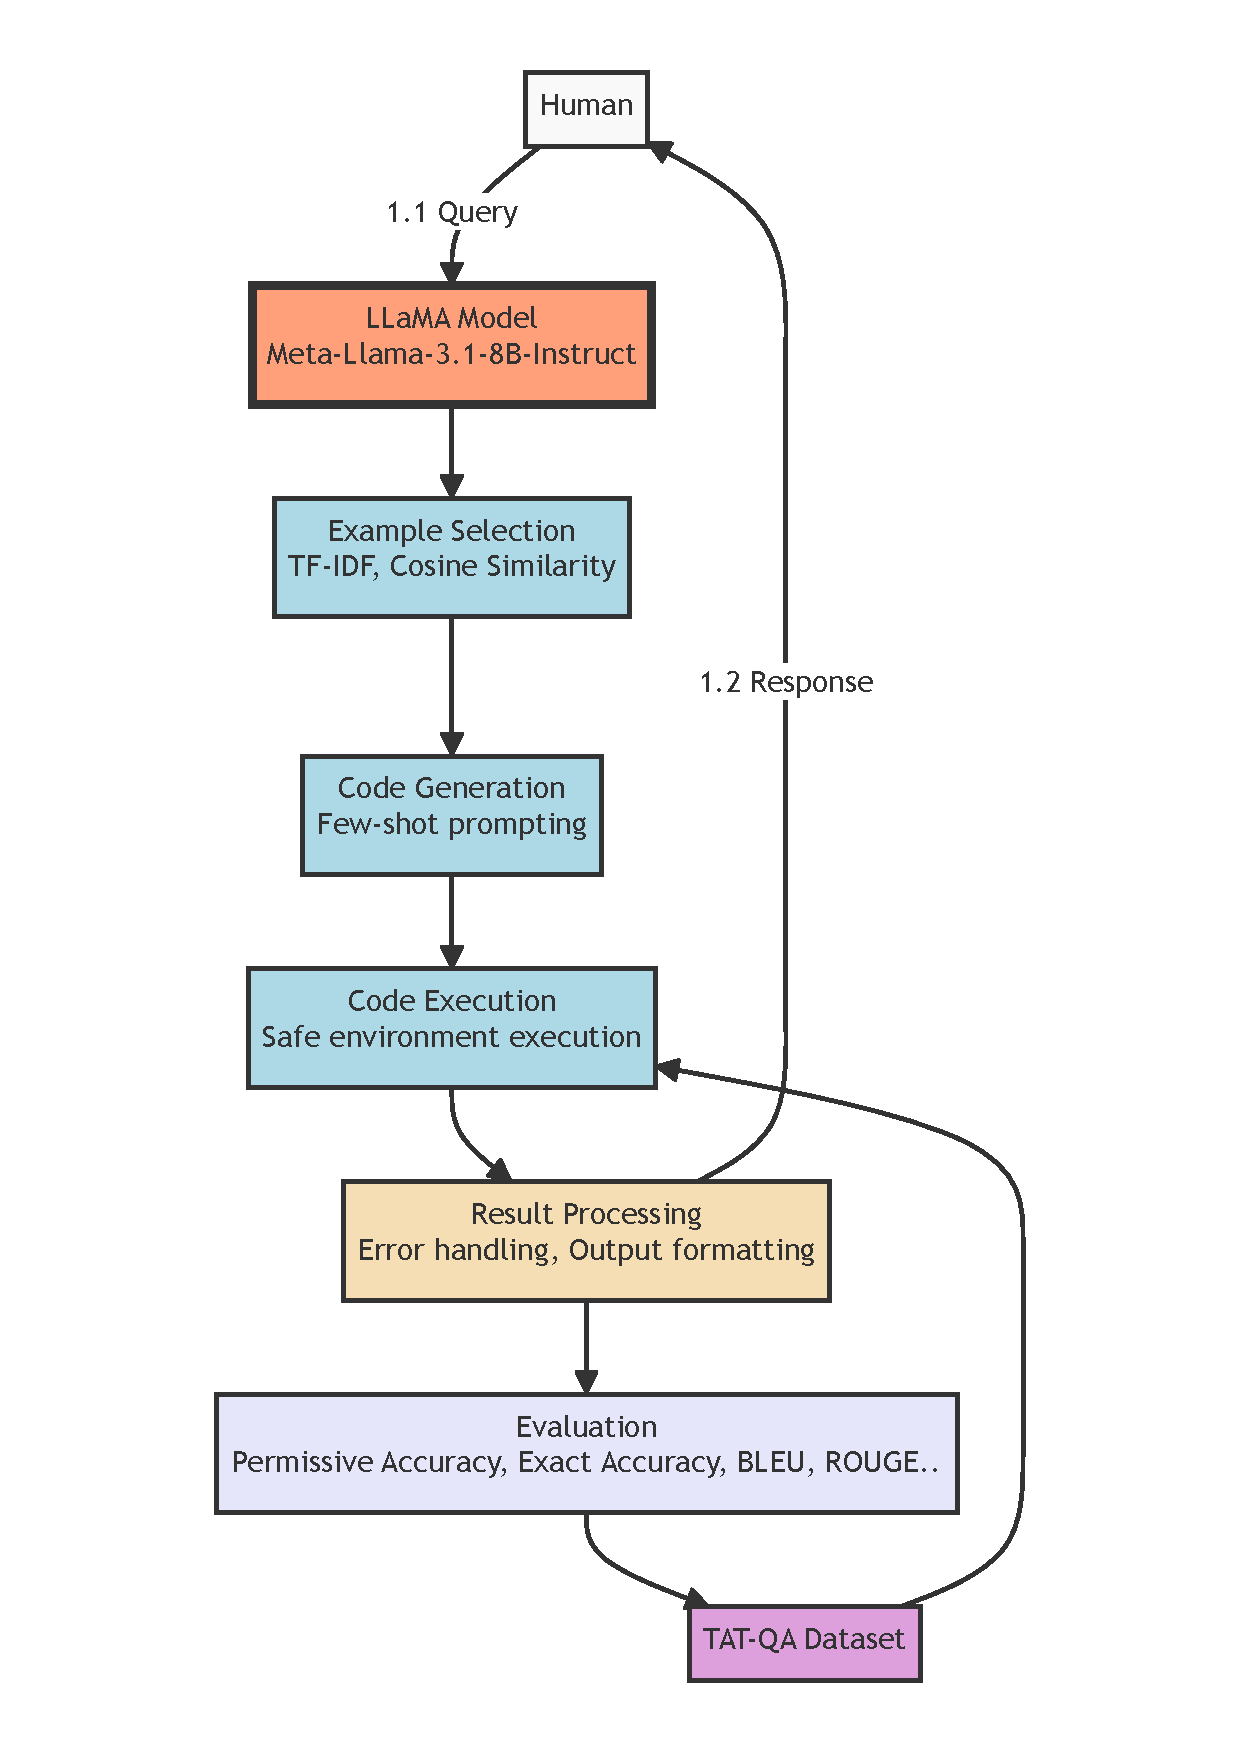
\includegraphics[width=0.60\linewidth]{mscdiss-skeleton/mermaid-diagram-updated.pdf}
    \caption{Workflow: Code Execution and Evaluation}
    \label{fig:methodology-flow}
\end{figure}
%This methodology represents a novel approach to financial data analysis, combining the power of advanced language models with domain-specific knowledge and real-time code execution. By dynamically generating and executing code based on natural language queries, our system demonstrates the potential for more flexible and accurate financial analysis tools.

\begin{comment}
\begin{figure}[!ht]
\centering
\resizebox{\textwidth}{!}{%
\begin{tikzpicture}[
    node distance = 0.8cm and 1.2cm,
    auto,
    thick,
    block/.style = {rectangle, draw, fill=white, text width=2cm, text centered, 
                    minimum height=0.8cm, font=\footnotesize, rounded corners},
    cloud/.style = {ellipse, draw, fill=white, text width=2cm, text centered, 
                    minimum height=0.8cm, font=\footnotesize},
    database/.style = {cylinder, draw, shape border rotate=90, aspect=0.25, fill=white, 
                       text width=2cm, text centered, minimum height=1.2cm, font=\footnotesize},
    line/.style = {draw, -{Stealth[scale=0.8]}, thick},
    dashed-line/.style = {draw, -{Stealth[scale=0.8]}, dashed, thick},
    group label/.style = {font=\tiny\bfseries, fill=white, draw, rounded corners, text centered, 
                          fill=gray!20, inner sep=1pt},
    group/.style = {rectangle, draw, rounded corners, fill=gray!10, inner sep=0.2cm}
]
% Input Processing
\node [cloud] (input) {Input Query};
\node [block, below=of input] (selection) {Example Selection};
\node [database, left=of selection, xshift=-0.8cm] (dataset) {TAT-QA Dataset};
% Code Generation
\node [block, below=of selection] (prompt) {Prompt Construction};
\node [block, below=of prompt] (generation) {Code Generation};
\node [cloud, left=of generation, xshift=-0.8cm] (model) {meta-llama/\\Meta-Llama-3.1-\\8B-Instruct};
\node [block, below=of generation] (extraction) {Code Extraction};
% Code Execution
\node [block, below=of extraction] (execution) {Code Execution};
\node [database, left=of execution, xshift=-0.8cm] (environment) {Execution Environment};
\node [block, below=of execution] (output) {Output Generation};
% Evaluation
\node [block, below=of output] (evaluation) {Evaluation of Results};
\node [database, left=of evaluation, xshift=-0.8cm] (metrics) {Metrics Suite};
% Connections
\path [line] (input) -- (selection);
\path [dashed-line] (dataset) -- (selection);
\path [line] (selection) -- (prompt);
\path [line] (prompt) -- (generation);
\path [dashed-line] (model) -- (generation);
\path [line] (generation) -- (extraction);
\path [line] (extraction) -- (execution);
\path [dashed-line] (environment) -- (execution);
\path [line] (execution) -- (output);
\path [line] (output) -- (evaluation);
\path [dashed-line] (metrics) -- (evaluation);
% Group boxes
\begin{pgfonlayer}{background}
    \node [group, fit=(input) (selection) (dataset)] (input-group) {};
    \node [group, fit=(prompt) (generation) (extraction) (model)] (generation-group) {};
    \node [group, fit=(execution) (output) (environment)] (execution-group) {};
    \node [group, fit=(evaluation) (metrics)] (evaluation-group) {};
\end{pgfonlayer}
% Group labels
\node [group label, above=0.05cm of input-group.north west, anchor=west] {Input Processing};
\node [group label, above=0.05cm of generation-group.north west, anchor=west] {Code Generation};
\node [group label, above=0.05cm of execution-group.north west, anchor=west] {Code Execution};
\node [group label, above=0.05cm of evaluation-group.north west, anchor=west] {Evaluation};
\end{tikzpicture}
}
\caption{Flowchart of the Code Generation Process for Financial Analysis}
\label{fig:methodology-flow}
\end{figure}
\end{comment}

%In the initial setup we choose a small handcrafted sampled from a variety of financial question-answer samples chosen from the dataset explained in section 4.1.1 . We then replaced the actual answers in the dataset with python scripts generated using the help of GPT-4 and verified manually. The sample of dataset were diverse and contains different representations like numerical answers or textual answer or date etc. To execute the Python scripts included in the answer fields, we utilised the LangChain LLM from the pipeline and then used the Python agent to run through a Python REPL (Read-Eval-Print Loop) tool. The Python REPL tool allows for real-time execution of Python code, which was crucial for dynamic and accurate computation of financial data. The model utilized for this integration was the Facebook 1.5b model, known for its robust language processing capabilities.

%\subsection{Subset Selection and Preparation}
%First, a small subset of the dataset was curated specifically for the LangChain integration. This subset was chosen to represent a variety of financial question-answer scenarios that required detailed computational analysis. Each entry in this subset included Python scripts in the answer fields, which were necessary for executing complex calculations. The selection criteria ensured that the subset contained diverse and representative examples that could test the model’s ability to handle different types of financial queries.

%\subsection{Python REPL Pipeline Integration}
%To execute the Python scripts included in the answer fields, the subset was run through a Python REPL (Read-Eval-Print Loop) pipeline. The Python REPL pipeline allows for real-time execution of Python code, which is crucial for dynamic and accurate computation of financial data. The model utilized for this integration was the Facebook 1.5b model, known for its robust language processing capabilities.

%\subsection{Integration Process}

%The integration process involved several technical steps:

%\begin{itemize}
    %\item Embedding Python Scripts: The Python scripts were embedded directly into the model prompts. This required careful formatting to ensure the scripts were correctly interpreted and executed by the REPL pipeline.
    %\item Model Adaptation: The Facebook 1.5b model was adapted to recognize and handle the embedded Python scripts. This adaptation involved training the model to parse the script correctly and execute it within the context of the financial question-answering task.
    %\item Output Handling: The outputs generated by the Python scripts were then reintegrated into the model’s response. This involved capturing the output from the REPL pipeline, formatting it appropriately, and ensuring it was included in the final answer provided by the model.
%\end{itemize}

%\subsection{Execution and Validation}
%During the inference phase, the integrated system worked as follows:

%\begin{itemize}
   % \item Query Processing: When a financial query was posed, the model parsed the question and identified the need for computational analysis.
    %\item Script Execution: The relevant Python script was executed using the Python REPL pipeline. This real-time execution allowed the model to handle complex calculations dynamically.
    %\item Result Integration: The results from the script execution were captured and formatted to be part of the model’s response. This integration ensured that the answer provided was accurate and directly addressed the computational aspects of the query.
%\end{itemize}
% \section{Other approaches used}

\chapter{Experiments}

This chapter delineates the framework, methodologies, and outcomes of our investigation, which focuses on enhancing the proficiency of language models in processing numerical data within financial contexts while also aiming for broad applicability across various financial tasks. We have employed a multifaceted approach that includes Instruction tuning, Few-shot prompting, Chain of Thought (CoT), and a hybrid strategy combining FSP and CoT, all designed to surpass the performance of existing models on diverse financial tasks. Additionally, we have pioneered a novel method that involves generating executable code from input data and processing it via the Python \textit{exec} function within a structured pipeline. An exhaustive discussion of these methodologies and their implications is presented in Section 5.3, providing a comprehensive insight into the advances and innovations introduced in our study.

\section{Research Questions}
Our experiments were designed to address the following research questions:
\begin{itemize}
\item How do Llama2-7B and Llama3-8B, model architectures with 7 billion and 8 billion parameters respectively, differ in baseline performance on financial tasks?
%\item What is the impact of fine-tuning on the models' performance across various metrics?
\item What is the relative effectiveness of various few-shot prompting strategies (e.g., zero-shot, one-shot, two-shot) compared to fine-tuning in enhancing model performance? Additionally, does the integration of Chain of Thought (CoT) techniques further influence the outcomes?

\item Is it possible to fine-tune a model to perform effectively across a variety of financial tasks? If so, which types of tasks remain the most challenging?

\item What is the optimal number of examples to use in few-shot prompting for financial tasks?
\item How does the performance of general-purpose language models on financial data processing tasks compare to that of specialized code generation approaches?
\end{itemize}

\section{Experimental Setup}

%\subsection{Dataset}
%We utilized a composite dataset combining four financial datasets which are explained in section 4.1 in detail. This diverse dataset allows us to evaluate model performance across various financial data types and tasks.

\subsection{Models}
\begin{comment}
We experimented with the following models:
\begin{itemize}
\item Llama2-7B chat (baseline and fine-tuned)
\item Llama3-8B (baseline and fine-tuned)
\item Llama3.1-8b (baseline) 
\item Llama3.1-8b-instruct (baseline)
\end{itemize}
\end{comment}
Our experiments were conducted using a series of progressively complex models to address the challenges posed by our dataset. Initially, we experimented with the Gemma-2b model; however, we quickly determined that its capacity was insufficient for the complexity inherent in our data, leading us to exclude it from our baseline assessments. Subsequent experiments commenced with the Llama2-7b-chat model. This decision was predicated on the observation that the base version, Llama2-7b, primarily excels in text completion tasks, while the chat variant offers enhanced flexibility through instruction tuning via system prompts. This feature allows for precise directive adjustments—for instance, directing the model to generate responses without supplementary explanations, tailored to the specific needs of our study. However, the limitations of the Llama2-7b model soon became apparent, particularly its restrictive context length, which proved inadequate for accommodating the extensive samples from our ConvFinQA dataset(see~\ref{convfinqa-sample-response} for example). Such constraints were also problematic for testing various Few-Shot Prompting (FSP) strategies, which necessitate the inclusion of additional examples in the input. Consequently, we transitioned to the Llama3-8b model for two pivotal reasons:
\begin{enumerate}
    \item The increased context length capabilities of the Llama3-8b model allowed for a more comprehensive exploration of our dataset, which was essential for the robust evaluation of different FSP approaches which includes relevant examples in addition to the long inputs. 
     \item The model's enhanced parameter size and training on a more contemporary dataset meant it demonstrated superior performance across reasoning and mathematical benchmarks compared to its predecessors.
\end{enumerate}
For the code generation aspect of our experiment, we selected the Llama3.1-8b variants, recognized for their superior code generation capabilities. This choice was crucial, as our research heavily relied on the model's ability to generate precise and accurate code outputs.

Furthermore, it is pertinent to note that the fine-tuning of these models was performed using their quantized versions, the specifics of which are detailed in~\ref{sec4.3.1}. 

\begin{comment}

\subsubsection{Approaches}

We implemented and compared several approaches:

\begin{enumerate}
  \item Baseline performance (zero-shot)
  \item Fine-tuning
  \item Few-shot prompting with chain-of-thought (FSP + CoT)
  \item Selective few-shot prompting
  \item Random few-shot prompting
  \item Tool-based approach using Langchain (on a subset of 150 samples)
   \item Code generation and execution (on TAT-QA dataset)
\end{enumerate}
\end{comment}
\begin{comment}
\subsection{Evaluation Metrics}
We employed a comprehensive set of metrics to evaluate model performance which are all detailed in section 4.4.3:
\begin{itemize}
\item Average Permissive Accuracy (custom metric allowing for slight numerical differences and partial text matches)
\item Average Exact Accuracy
\item ROUGE Score
\item BLEU Score
\item METEOR Score
\item BERTScore (Precision, Recall, F1)
\item GLEU Score
\end{itemize}
\begin{figure}[h!] 
    \centering 
    \includegraphics[width=0.75\textwidth]{mscdiss-skeleton/Screenshot 2024-08-04 at 19.20.50.png} 
    \caption{Performance Metrics of various models} 
    \label{fig:my_label} 
\end{figure}
\end{comment}

\section{Results and Analysis}
\subsection{Model Architecture Comparison}
%Table 5.1 presents the evaluation metrics for various models and approaches.

\begin{table}[h!]
\centering
\caption{Evaluation Metrics for Fine tuned Models}
\label{table:metrics-fine-tuned}
\resizebox{\textwidth}{!}{%
\begin{tabular}{@{}lccccccccc@{}}
\toprule
Model & Avg Permissive Acc. & Avg Exact Acc. & ROUGE Score & BLEU Score & METEOR Score & BERTScore P & BERTScore R & BERTScore F1 & GLEU Score \\ 
\midrule
%Llama2-7B chat baseline & 0.2720 & 0.0225 & 0.16 & 0.01 & 0.19 & 0.814 & 0.860 & 0.836 & 0.02 \\
Llama2-7B chat baseline & 0.27 & 0.02 & 0.16 & 0.01 & 0.19 & 0.814 & 0.860 & 0.836 & 0.02 \\
Llama3-8B baseline & 0.33 & 0.05 & 0.20 & 0.03 & 0.19 & 0.836 & 0.876 & 0.855 & 0.04 \\
Llama2-7B chat Fine tuned & 0.46 & 0.00 & 0.15 & 0.05 & 0.21 & 0.778 & 0.892 & 0.830 & 0.07 \\
Llama3-8B Fine tuned & \textbf{0.67} & 0.15 & 0.36 & 0.06 & \textbf{0.31} & 0.850 & 0.919 & 0.881 & 0.07 \\
Llama3-8B - CoT  & 0.63 & 0.14 & 0.35 & 0.07 & 0.31 & 0.847 & 0.918 & 0.879 & 0.07 \\
Llama3-8B - FSP+CoT (Zero shot) & 0.62 & \textbf{0.16} & \textbf{0.38} & \textbf{0.07} & \textbf{0.31} & \textbf{0.863} & \textbf{0.921} & \textbf{0.890} & \textbf{0.08} \\
Llama3-8B - FSP+CoT (One shot)  & 0.62 & 0.16 & 0.37 & 0.07 & 0.31 & 0.861 & 0.921 & 0.889 & 0.08 \\
Llama3-8B - FSP+CoT (Two shot)  & 0.62 & 0.15 & 0.37 & 0.07 & 0.31 & 0.859 & 0.921 & 0.887 & 0.07 \\
Llama3-8B - FSP+CoT (Random)  & 0.62 & 0.16 & 0.37 & 0.07 & 0.31 & 0.860 & 0.920 & 0.887 & 0.07 \\
Llama3-8B - FSP+CoT (Mix Shot)  & 0.62 & 0.16 & 0.37 & 0.07 & 0.31 & 0.859 & 0.920 & 0.887 & 0.08 \\


%Llama3-8B Selective FSP & 0.64 & 0.11 & 0.27 & 0.06 & 0.28 & 0.809 & 0.913 & 0.855 & 0.05 \\
%Llama3-8B Random FSP & 0.64 & 0.11 & 0.27 & 0.06 & 0.28 & 0.807 & 0.912 & 0.854 & 0.05 \\
%LLAMA3-8B {Zero shot, one shot, five shot.. } & Separate table & - & - & - & - & - & - & - & - \\
%Tool use Langchain [150 samples] & - & 0.75 & 0.30 & 0.23 & 0.33 & 0.822 & 0.878 & 0.849 & 0.23 \\
\bottomrule
\end{tabular}
}
\end{table}

In the series of experiments mentioned in \ref{table:metrics-fine-tuned}, we investigated the performance of two open source language models i.e. Llama2 \& Llama3 across various configurations and few-shot prompting strategies, focusing on their application in our merged dataset. The analysis of Llama2-7B and Llama3-8B models revealed that the Llama3-8B model, with its additional billion parameters, exhibited a superior baseline performance. Specifically, it demonstrated a 22.2\% increase in Average Permissive Accuracy and a 150\% increase in Average Exact Accuracy over the Llama2-7B model. These enhancements are attributed to the increased computational capabilities and broader contextual understanding afforded by the larger model size.

\begin{comment}
    
\begin{figure}[h!]
    \centering
    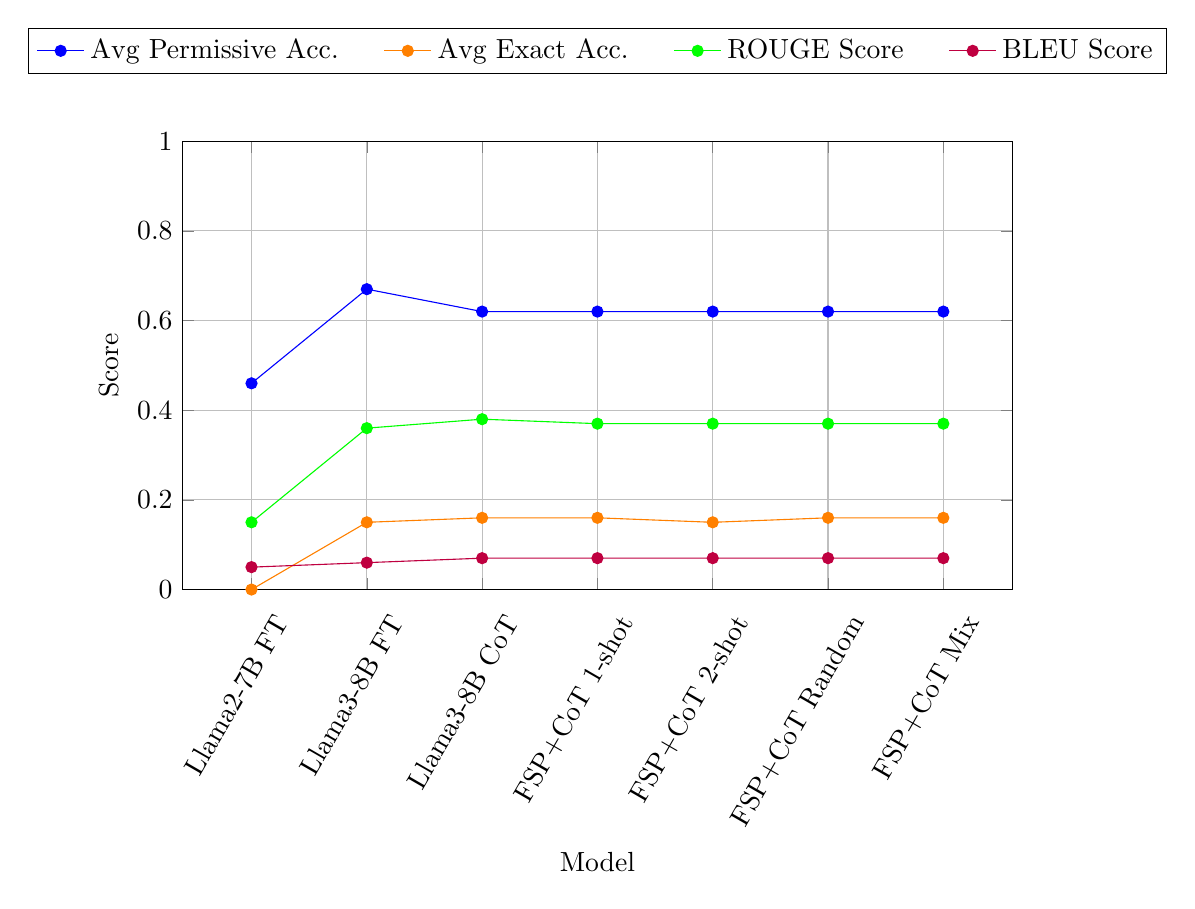
\begin{tikzpicture}
        \begin{axis}[
            width=\textwidth,
            height=0.6\textwidth,
            xlabel={Model},
            ylabel={Score},
            xtick={1,2,3,4,5,6,7},
            xticklabels={Llama2-7B FT, Llama3-8B FT, Llama3-8B CoT, FSP+CoT 1-shot, FSP+CoT 2-shot, FSP+CoT Random, FSP+CoT Mix},
            xticklabel style={rotate=60, anchor=east, yshift=-0.5cm},
            legend style={at={(0.5,1.15)}, anchor=south,legend columns=-1,/tikz/every even column/.append style={column sep=0.5cm}},
            grid=major,
            ymin=0, ymax=1,
            ]

            % Avg Permissive Acc.
            \addplot[color=blue, mark=*] coordinates {
                (1, 0.46)
                (2, 0.67)
                (3, 0.62)
                (4, 0.62)
                (5, 0.62)
                (6, 0.62)
                (7, 0.62)
            };
            \addlegendentry{Avg Permissive Acc.}

            % Avg Exact Acc.
            \addplot[color=orange, mark=*] coordinates {
                (1, 0.00)
                (2, 0.15)
                (3, 0.16)
                (4, 0.16)
                (5, 0.15)
                (6, 0.16)
                (7, 0.16)
            };
            \addlegendentry{Avg Exact Acc.}

            % ROUGE Score
            \addplot[color=green, mark=*] coordinates {
                (1, 0.15)
                (2, 0.36)
                (3, 0.38)
                (4, 0.37)
                (5, 0.37)
                (6, 0.37)
                (7, 0.37)
            };
            \addlegendentry{ROUGE Score}

            % BLEU Score
            \addplot[color=purple, mark=*] coordinates {
                (1, 0.05)
                (2, 0.06)
                (3, 0.07)
                (4, 0.07)
                (5, 0.07)
                (6, 0.07)
                (7, 0.07)
            };
            \addlegendentry{BLEU Score}

        \end{axis}
    \end{tikzpicture}
    \caption{Line Plot for Fine-tuned Models}
    \label{fig:lineplot-fine-tuned}
\end{figure}


\begin{figure}[htbp]
\centering
\begin{tikzpicture}
\pgfplotsset{
    width=0.45\textwidth,
    height=0.3\textheight,
    ybar,
    bar width=7pt,
    symbolic x coords={FT,CoT,Zero,One,Two,Random,Mix},
    xtick=data,
    xticklabel style={rotate=45,anchor=east},
    ylabel near ticks,
    ymajorgrids,
    nodes near coords,
    nodes near coords style={font=\tiny, rotate=90, anchor=west},
    legend style={font=\tiny},
    title style={font=\small}
}

% Avg. Permissive Accuracy
\begin{axis}[
    ymin=0.6, ymax=0.7,
    title={Avg. Permissive Accuracy},
    at={(0,0.5\textheight)}
]
\addplot[fill=blue!60] coordinates {
    (FT,0.67) (CoT,0.63) (Zero,0.62) (One,0.62) (Two,0.62) (Random,0.62) (Mix,0.62)
};
\end{axis}

% Exact Accuracy
\begin{axis}[
    ymin=0.13, ymax=0.17,
    title={Avg. Exact Accuracy},
    at={(0.5\textwidth,0.5\textheight)}
]
\addplot[fill=red!60] coordinates {
    (FT,0.15) (CoT,0.14) (Zero,0.16) (One,0.16) (Two,0.15) (Random,0.16) (Mix,0.16)
};
\end{axis}

% ROUGE Score
\begin{axis}[
    ymin=0.34, ymax=0.39,
    title={ROUGE Score},
    at={(0,0)}
]
\addplot[fill=green!60] coordinates {
    (FT,0.36) (CoT,0.35) (Zero,0.38) (One,0.37) (Two,0.37) (Random,0.37) (Mix,0.37)
};
\end{axis}

% BLEU Score
\begin{axis}[
    ymin=0.05, ymax=0.08,
    title={BLEU Score},
    at={(0.5\textwidth,0)}
]
\addplot[fill=orange!60] coordinates {
    (FT,0.06) (CoT,0.07) (Zero,0.07) (One,0.07) (Two,0.07) (Random,0.07) (Mix,0.07)
};
\end{axis}

\end{tikzpicture}
\caption{Evaluation Metrics for Selected Llama3-8b Models}
\label{fig:evaluation_metrics}
\end{figure}
\end{comment}

\begin{figure}[htbp]
\centering
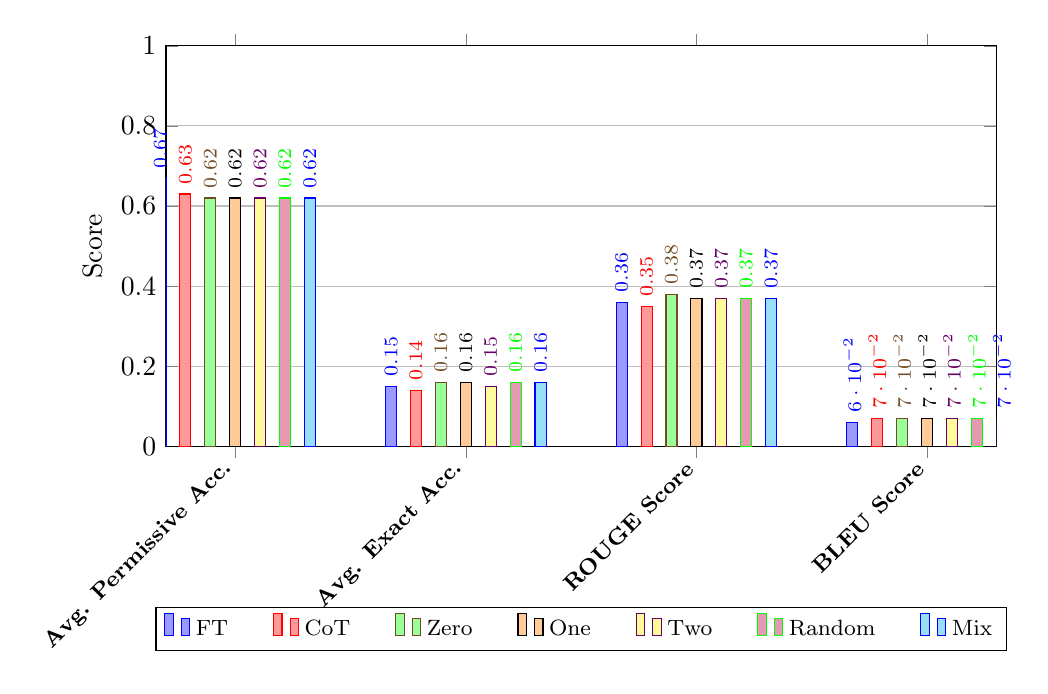
\begin{tikzpicture}
\begin{axis}[
    width=1.0\textwidth,
    height=0.55\textwidth,
    ybar=5pt,
    bar width=4pt,
    ylabel={Score},
    enlarge x limits=0.1,
    symbolic x coords={Avg. Permissive Acc., Avg. Exact Acc., ROUGE Score, BLEU Score},
    xtick=data,
    xticklabel style={rotate=45, anchor=east, font=\footnotesize\bfseries},
    legend style={at={(0.5,-0.4)}, % Moved legend further down
        anchor=north,legend columns=7, % Changed to 4 columns
        font=\footnotesize,
        /tikz/every even column/.append style={column sep=0.5cm}}, % Added space between legend columns
    ylabel near ticks,
    ymin=0,
    ymax=1,
    ytick={0,0.2,0.4,0.6,0.8,1.0},
    ymajorgrids,
    %title={Evaluation Metrics for Selected Llama3-8b Models},
    %title style={font=\bfseries},
    every node near coord/.append style={font=\scriptsize, rotate=90, anchor=west},
    nodes near coords={\pgfmathprintnumber[fixed zerofill, precision=2]{\pgfplotspointmeta}},
]
\addplot+[ybar, fill=blue!40] coordinates {
    (Avg. Permissive Acc., 0.67) % FT
    (Avg. Exact Acc., 0.15) % FT
    (ROUGE Score, 0.36) % FT
    (BLEU Score, 0.06) % FT
};
\addplot+[ybar, fill=red!40] coordinates {
    (Avg. Permissive Acc., 0.63) % CoT
    (Avg. Exact Acc., 0.14) % CoT
    (ROUGE Score, 0.35) % CoT
    (BLEU Score, 0.07) % CoT
};
\addplot+[ybar, fill=green!40] coordinates {
    (Avg. Permissive Acc., 0.62) % Zero
    (Avg. Exact Acc., 0.16) % Zero
    (ROUGE Score, 0.38) % Zero
    (BLEU Score, 0.07) % Zero
};
\addplot+[ybar, fill=orange!40] coordinates {
    (Avg. Permissive Acc., 0.62) % One
    (Avg. Exact Acc., 0.16) % One
    (ROUGE Score, 0.37) % One
    (BLEU Score, 0.07) % One
};
\addplot+[ybar, fill=yellow!40] coordinates {
    (Avg. Permissive Acc., 0.62) % Two
    (Avg. Exact Acc., 0.15) % Two
    (ROUGE Score, 0.37) % Two
    (BLEU Score, 0.07) % Two
};
\addplot+[ybar, fill=purple!40] coordinates {
    (Avg. Permissive Acc., 0.62) % Random
    (Avg. Exact Acc., 0.16) % Random
    (ROUGE Score, 0.37) % Random
    (BLEU Score, 0.07) % Random
};
\addplot+[ybar, fill=cyan!40] coordinates {
    (Avg. Permissive Acc., 0.62) % Mix
    (Avg. Exact Acc., 0.16) % Mix
    (ROUGE Score, 0.37) % Mix
    (BLEU Score, 0.07) % Mix
};
\legend{FT, CoT, Zero, One, Two, Random, Mix}
\end{axis}
\end{tikzpicture}
\caption{Evaluation Metrics for Selected Llama3-8b Models}
\label{fig:evaluation_metrics}
\end{figure}

Further experiments employed few-shot prompting strategies and the integration of Few Shot Prompting (FSP) \& Chain of Thought (CoT) techniques. Notably, the fine-tuned Llama3-8B model showed remarkable improvement, achieving a 67\% Average Permissive Accuracy, representing a substantial enhancement from its baseline performance. Moreover, the FSP+CoT Zero-shot configuration notably excelled, achieving the highest increases across several metrics including a 90.00\% rise in ROUGE Score and a 133.33\% increase in BLEU Score compared to the baseline Llama3-8B model. In terms of Exact Accuracy, the FSP+CoT Zero-shot approach demonstrates a 6.67\% improvement over the comparably optimized fine-tuned Llama3-8B model, underscoring its enhanced efficacy in precise response generation. 
%These results underscore the efficacy of CoT techniques in structuring the model’s reasoning process, thereby enhancing performance.

For the few-shot prompting approach, we employed the relevant examples algorithm detailed in algorithm~\ref{alg:precomputeExamples}. The \textsc{few\_shot\_examples} function received 20 selectively chosen examples from the four datasets utilized in our experiments. These examples were specifically modified to differ from those used in the fine-tuning process; notably, for the TAT-QA, ConvFinQA, and FinQA datasets, the answer field was adapted to include step-by-step responses rather than a singular, final answer. In contrast, for relation extraction tasks, the examples remained akin to the training samples, focusing on direct extraction from provided information without necessitating stepwise reasoning. It is pertinent to highlight that all experimental results reported in~\ref{table:metrics-fine-tuned} were derived from testing on a comprehensive dataset comprising 1287 samples, which collectively encompass elements from all four datasets involved in the study.

In addressing our second research question regarding the efficacy of various few-shot prompting strategies and the potential enhancement provided by the Chain of Thought (CoT) technique, our analysis yielded intriguing results. Interestingly, it is observed that CoT approach independently couldn't perform as good as when it is used in combination with different few shot approaches. Contrary to expectations, we observed no substantial performance differences when the model was prompted with either random or relevant examples, or even without any specific examples (zero-shot). This lack of differential suggests a performance plateau from tailored example inputs, which might be attributed to several factors: potential saturation in the model's learning capability from few-shot examples, the model's high baseline abilities resulting from extensive pre-training, and the complex nature of financial tasks which may require more than mere contextual cues provided by few-shot examples. Regarding the integration with CoT, our results demonstrated noticeable enhancements in Exact Match Accuracy along with other critical metrics, including ROUGE, BLEU, METEOR, BERT, and GLEU Scores. These improvements establish CoT in conjunction with zero shot prompting as the superior approach, notwithstanding its marginally lesser performance in terms of Permissive Accuracy. These metrics are crucial for evaluating the model's performance as they assess the congruence between the predicted responses and the references, encompassing a variety of aspects. This is particularly pertinent given that our generated responses are not solely numerical but also include a significant proportion of textual answers, especially prevalent within the relation extraction dataset.

The decision to explore various few-shot strategies, despite the similar outcomes, was driven by the intent to rigorously test the model’s adaptability to different instructional contexts. This was essential to identify any potential nuances in how different prompting strategies might affect performance. While these strategies did not yield the expected variance in results, they provided valuable insights into the limitations and capabilities of current LLMs in handling complex tasks like financial analysis. 

\begin{comment}
\textbf{Key observations:}
\begin{itemize}
 \item Llama3-8B baseline outperforms Llama2-7B chat baseline across all metrics, indicating that the newer architecture has inherently better number handling capabilities.
 \item The performance gap is particularly noticeable in Average Permissive Accuracy (0.33 vs. 0.27) and Average Exact Accuracy (0.05 vs. 0.02).
\end{itemize}
\subsection{Impact of Fine-tuning}
\textbf{Fine-tuning significantly improved the performance of both model architectures:}
\begin{itemize}

\item Llama2-7B chat: Average Permissive Accuracy increased from 0.27 to 0.46
\item Llama3-8B: Average Permissive Accuracy increased from 0.33 to 0.67

The fine-tuned Llama3-8B model showed the best overall performance, with notable improvements in ROUGE Score (0.36) and METEOR Score (0.31).
\end{itemize}
\end{comment}
\subsection{Few-shot Prompting on individual datasets} 
In this analysis, we conduct a detailed examination of the Few-Shot Prompting approach, assessing its performance across individual datasets and corresponding metrics. It is critical to emphasize that the evaluations for each dataset were performed on their respective test sets, ensuring that the results presented are dataset-specific and not generalized across all datasets included in this study. The model employed for inference in this study was consistent with the one utilized in prior experiments; specifically, it was fine-tuned using the Chain of Thought (CoT) and Few-Shot Prompting (FSP) approaches. This fine tuned model utilises either 0, 1 or 2 relevant examples, which were selected randomly to optimize its performance and applicability to the tasks at hand.

\begin{table}[h!]
\centering
\caption{Evaluation Results on TAT-QA dataset}
\label{table:metrics-FSP-Indv-tat}
\resizebox{\textwidth}{!}{%
\begin{tabular}{@{}lccccccccc@{}}
\toprule
Approach & Avg Permissive Acc. & Avg Exact Acc. & ROUGE Score & BLEU Score & METEOR Score & BERTScore P & BERTScore R & BERTScore F1 & GLEU Score \\ 
\midrule
Zero Shot &  0.59 & \textbf{0.14} & \textbf{0.43} & \textbf{0.12} & \textbf{0.30} & \textbf{0.869} & \textbf{0.922} & \textbf{0.894} & \textbf{0.12}\\
One Shot &   \textbf{0.60} & 0.13 & 0.41 & 0.11 & 0.29 & 0.863 & 0.920 & 0.889 & 0.11\\
Two Shot & \textbf{0.60} & 0.12 & 0.39 & 0.11 & 0.29 & 0.859 & 0.918 & 0.886 & 0.10     \\
Random Shot  &  0.59 & 0.13 & 0.41 & 0.11 & 0.29 & 0.863 & 0.919 & 0.889 & 0.11     \\
Mix Shot      & 0.59 & 0.13 & 0.40 & 0.11 & 0.29 & 0.860 & 0.918 & 0.887 & 0.10     \\
\bottomrule
\end{tabular}
}
\end{table}
\begin{table}[h!]
\centering
\caption{Evaluation Results on ConvFinQA Dataset}
\label{table:metrics-FSP-Indv-ConvFinQA}
\resizebox{\textwidth}{!}{%
\begin{tabular}{@{}lccccccccc@{}}
\toprule
Approach & Avg Permissive Acc. & Avg Exact Acc. & ROUGE Score & BLEU Score & METEOR Score & BERTScore P & BERTScore R & BERTScore F1 & GLEU Score \\ 
\midrule
Zero Shot & \textbf{0.68} & \textbf{0.56} & \textbf{0.78} & 0.00 & 0.28 & \textbf{0.977} & 0.975 & \textbf{0.976} & 0.27 \\
One Shot & \textbf{0.68} & \textbf{0.56} & \textbf{0.78} & 0.00 & 0.28 & 0.976 & 0.975 & \textbf{0.976} & \textbf{0.34} \\
Two Shot & 0.67 & \textbf{0.56} & 0.77 & 0.00 & 0.28 & 0.976 & 0.975 & 0.975 & 0.31 \\
Random Shot & \textbf{0.68} & \textbf{0.56} & \textbf{0.78} & 0.00 & 0.28 & \textbf{0.977} & 0.975 & \textbf{0.976} & 0.27 \\
Mix Shot & \textbf{0.68} & \textbf{0.56} & \textbf{0.78} & 0.00 & 0.28 & 0.976 & 0.975 & 0.975 & 0.32 \\
\bottomrule
\end{tabular}
}
\end{table}
\begin{table}[h!]
\centering
\caption{Evaluation Results on FinQA Dataset}
\label{table:metrics-FSP-Indv-FINQA}
\resizebox{\textwidth}{!}{%
\begin{tabular}{@{}lccccccccc@{}}
\toprule
Approach & Avg Permissive Acc. & Avg Exact Acc. & ROUGE Score & BLEU Score & METEOR Score & BERTScore P & BERTScore R & BERTScore F1 & GLEU Score \\ 
\midrule
Zero Shot & \textbf{0.30} & \textbf{0.02} & \textbf{0.12} & 0.00 & \textbf{0.10} & \textbf{0.810} & 0.806 & 0.803 & 0.01 \\
One Shot & 0.28 & \textbf{0.02} & 0.11 & 0.00 & 0.09 & \textbf{0.810} & 0.806 & \textbf{0.804} & 0.01 \\
Two Shot & 0.28 & \textbf{0.02} & 0.10 & 0.00 & 0.09 & 0.806 & \textbf{0.807} & 0.801 & 0.01 \\
Random Shot & 0.29 & \textbf{0.02} & 0.10 & 0.00 & 0.09 & 0.804 & 0.806 & 0.800 & 0.01 \\
Mix Shot & 0.29 & \textbf{0.02} & 0.11 & 0.00 & \textbf{0.10} & 0.808 & \textbf{0.807} & 0.802 & 0.01 \\
\bottomrule
\end{tabular}
}
\end{table}
\begin{table}[h!]
\centering
\caption{Evaluation Results on Relation-Extraction Dataset}
\label{table:metrics-FSP-Indv-RelationExtraction}
\resizebox{\textwidth}{!}{%
\begin{tabular}{@{}lccccccccc@{}}
\toprule
Approach & Avg Permissive Acc. & Avg Exact Acc. & ROUGE Score & BLEU Score & METEOR Score & BERTScore P & BERTScore R & BERTScore F1 & GLEU Score \\ 
\midrule
Zero Shot & \textbf{0.85} & 0.00 & \textbf{0.19} & \textbf{0.05} & \textbf{0.40} & \textbf{0.817} & \textbf{0.899} & \textbf{0.856} & 0.09 \\
One Shot & \textbf{0.85} & 0.00 & \textbf{0.19} & \textbf{0.05} & 0.39 & \textbf{0.817} & 0.898 & 0.855 & 0.09 \\
Two Shot & 0.84 & 0.00 & \textbf{0.19} & \textbf{0.05} & 0.39 & \textbf{0.817} & 0.898 & 0.855 & 0.09 \\
Random Shot & \textbf{0.85} & 0.00 & \textbf{0.19} & \textbf{0.05} & \textbf{0.40} & \textbf{0.817} & \textbf{0.899} & \textbf{0.856} & 0.09 \\
Mix Shot & 0.84 & 0.00 & \textbf{0.19} & \textbf{0.05} & 0.39 & \textbf{0.817} & 0.898 & 0.855 & 0.09 \\
\bottomrule
\end{tabular}
}
\end{table}
%Our findings on the TAT-QA dataset indicate that while there is a slight improvement with increased prompting, the gains are marginal, suggesting a plateau in performance enhancement through few-shot methods. The highest observed Average Permissive Accuracy was 0.60 for one and two-shot scenarios. However, the low Exact Accuracy rates across these configurations highlight  challenges in achieving precise numerical reasoning. These results are more in line with the table 5.1 reiterating that Zero shot performance is the overall best metric when dealing with tabular mixed with textual data and strengthening the case that Chain of Thought approach works well independent of using examples. 
The results from the TAT-QA dataset indicated that while there was a slight improvement with increased prompting, the gains were marginal, pointing to a potential plateau in performance enhancement achievable through few-shot methods. This was particularly evident as the highest Average Permissive Accuracy reached was 0.60 for one and two-shot scenarios. However, the consistently low Exact Accuracy rates across these configurations underscored significant challenges in achieving precise numerical reasoning. These observations are consistent with earlier results \ref{table:metrics-fine-tuned}, which highlighted that the Zero Shot performance generally yielded the best outcomes when dealing with data that integrates tabular content with textual data, thereby reinforcing the effectiveness of the Chain of Thought (CoT) approach regardless of the use of examples.
In the ConvFinQA dataset, the models demonstrated robust performance, consistently achieving high Permissive Accuracies around 0.68 and Exact Accuracies at 0.56 across most approaches. This dataset, which benefits from not truncating inputs despite longer context lengths, showcased our tuned models' strong performance in understanding QA history—a task generally considered challenging. Notably, these results did not significantly differ across the few-shot prompting variations, which highlighted a potential limitation in the impact of adding more contextual examples within datasets well-aligned with the models' training. Additionally, an unexpected observation was the consistent 0 scores for the BLEU Score metric in both the ConvFinQA and FinQA datasets. Upon further investigation, it was revealed that these scores reflect the limitations of applying the BLEU score metric, traditionally designed for corpus-level evaluation, to single predictions and references. As Wu et al. (2016) identified, the BLEU score exhibits several undesirable properties when utilized for single sentences \cite{wu2016googles}. Consequently, we have also reported the GLEU Score, which is designed to mitigate these undesirable properties when assessing single sentences. This adjustment provides a more appropriate measure of accuracy in contexts where traditional metrics such as BLEU may not be applicable.
%Similarly, in the ConvFinQA dataset, the models demonstrated robust performance, consistently achieving high Permissive Accuracies around 0.68 and Exact Accuracies at 0.56 across most approaches. The idea of not truncating inputs despite longer context lengths helps as shown by high permissive and exact accuracies. These results also implies our tuned models strong performance in understanding QA history which in general is considered a challenging task. However, this did not significantly differ across the few-shot prompting variations, underscoring a potential limitation in the impact of adding more contextual examples within well-aligned datasets.

The FinQA dataset presented considerable challenges, with Permissive Accuracies barely under 0.30 and negligible Exact Accuracy. This dataset, based on earnings reports from S&P 500 companies, necessitates a high degree of inferential reasoning. For example, questions such as \emph{Considering the weighted average fair value of options, what was the change of shares vested from 2005 to 2006?} require the model to calculate the number of shares and select relevant numbers from both the table and the text to generate the reasoning program to arrive at the answer \cite{chen2021finqa}, which remains a substantial hurdle, indicating the model's shortcomings in complex text understanding and information extraction from dense financial narratives. To answer our third research question, we can say that although the model demonstrated a 6.67\% improvement over the fine-tuned Llama-3-8b model in terms of exact match on the merged test set, thus improving performance across diverse financial tasks, the FinQA questions remain the most challenging for the model \ref{table:metrics-FSP-Indv-FINQA}. Further analysis and research are needed to enhance the model's performance on this specific dataset.

The findings from the Relation-Extraction dataset unveiled a pronounced discrepancy between high Permissive Accuracy and zero Exact Accuracy, illustrating a critical challenge in the model's ability to execute precise relation extraction. Although the model demonstrated competency in broadly identifying correct relational concepts, it faltered in accurately pinpointing and extracting the most relevant relations. This challenge is exemplified by the model's response to structured prompts designed to extract the single most prominent relation. For instance, given the context from a news conference by JPMorgan Chase & Co's CEO, Jamie Dimon, the model was instructed to identify specific relationships within the sentence. Despite the intended response being \emph{employer: Jamie Dimon, JPMorgan Chase}, the model provided an overly comprehensive array of relational data, including multiple unrelated relations such as \emph{position held: Jamie Dimon, Chief Executive Officer} among others (see~\ref{rel-extraction-sample} for a complete example). This overflow of information suggests that while the model can recognize relational data, it tends to overgeneralize from the input, leading to responses that extend beyond the required extraction. This issue could potentially be mitigated by refining the model's prompt structure to more clearly delineate the expected response boundaries, yet the dataset inherently demands multiple extractions per instance, complicating the clarity of how many relations are to be extracted. This complexity necessitated the introduction of an additional metric, Average Permissive Accuracy, to provide a more lenient measure of the model's performance, acknowledging that while not exactly precise, the model successfully captures the correct answers a significant portion of the time. Despite this adaptation, we continue to report the Exact Match Accuracy to maintain a rigorous standard of evaluation and to transparently assess the model's precision in relation extraction tasks.

%Addressing the effectiveness of few-shot prompting (FSP) in financial tasks, our studies across multiple datasets reveal that increasing the number of few-shot examples does not necessarily lead to substantial performance enhancements. This observation suggests that the quality and relevance of examples—particularly their alignment with specific task requirements—may be more impactful than simply increasing the quantity of examples. In instances where few-shot prompting failed to improve performance, the inherent complexity and specificity of the tasks likely diminished the added value of more examples. This finding highlights a crucial direction for our future research, emphasizing the need to refine the strategic use of few-shot examples to enhance model performance effectively.
%Furthermore, results from the Relation-Extraction dataset revealed high Permissive Accuracy but zero Exact Accuracy. This discrepancy indicates that while the model can broadly identify correct relational concepts, it struggles with exact relation extraction. This is attributed to the fact that even when we prompt the model to extract single most prominent relation (Prompt structure ref -Appendix), it focuses more on the input question which direct it to various options for eg: if the context is 'Detailed results will likely be released by the banks to shareholders on Friday, JPMorgan Chase & Co Chief Executive Jamie Dimon said at a news conference.' and the question is 'Given the input sentence, please extract the subject and object containing a certain relation in the sentence according to the following relation types, in the format of \"relation1: word1, word2; relation2: word3, word4\". Relations include: product/material produced; manufacturer; distributed by; industry; position held; original broadcaster; owned by; founded by; distribution format; headquarters location; stock exchange; currency; parent organization; chief executive officer; director/manager; owner of; operator; member of; employer; chairperson; platform; subsidiary; legal form; publisher; developer; brand; business division; location of formation; creator.', the reference answer is 'employer: Jamie Dimon, JPMorgan Chase' but the models response is ' employer: Jamie Dimon, JPMorgan Chase; position\_held: Jamie Dimon, Chief Executive Officer; employer: Jamie Dimon, JPMorgan Chase; chief\_executive\_officer: JPMorgan Chase, Jamie Dimon; position\_held: Jamie Dimon, CEO; employer: Jamie Dimon, JPMorgan Chase; location\_of\_formation: JPMorgan Chase, New York City; headquarters\_location: JPMorgan Chase, New York City'. We could truncate the response to one extraction but the dataset contains samples where more than one extraction is required and it is not clear how many relations are required though we tried to fix this using instruction tuning to extract most relevant prompts the model give more weight to the question and hence the additional metric we introduced i.e. Average Permissive Accuracy since just using exact metric will give 0 for all the realtion extraction samples which is not necessarily the case since the model is able to gather the correct answer almost 85\% of times and since these are not numerical values we gave this much of leeway to the model but we do report the exact accuracy. 

Revisiting the research question on the optimal number of examples for Few-Shot Prompting (FSP) in financial tasks, our findings reveal that increasing the number of examples does not consistently lead to significant performance gains across all datasets. This suggests that the quality and relevance of examples, particularly in designing prompts that closely reflect task-specific requirements, may be more crucial than merely increasing the number of examples provided. Furthermore, our experiments indicate that the Chain-of-Thought (CoT) approach performs effectively even with zero shots, \emph{suggesting that the combination of FSP with examples and CoT is not always necessary, particularly for complex tasks where the model tends to rely more on training data than on a few new examples provided during inference}. In cases where few-shot prompting did not enhance performance, it is likely that the complexity and specificity of the tasks diminish the benefits of additional examples, highlighting an important area for future research.

\begin{comment}
    
Different few-shot prompting strategies yielded varying results:
\begin{itemize}

\item FSP + CoT: Achieved high performance (0.59 Average Permissive Accuracy) but did not surpass fine-tuned models.
\item Selective FSP and Random FSP: Both achieved 0.64 Average Permissive Accuracy, indicating that careful example selection may not always be necessary.
\end{itemize}

\subsection{Optimal Few-shot Prompting}
Table 5.2 shows the performance metrics for different few-shot prompting approaches.
%Change this table based on new experiments on random, selective and zero examples
\begin{table}[h!]
\centering
\caption{Performance Metrics for Different Few Shot Prompting}
\label{tab:performance_metrics}
\resizebox{\textwidth}{!}{%
\begin{tabular}{@{}lccccccccc@{}}
\toprule
Fine Tuning Type & Avg Permissive Acc. & Avg Exact Acc. & ROUGE Score & BLEU Score & METEOR Score & BERTScore P & BERTScore R & BERTScore F1 & GLEU Score \\ 
\midrule
1 Relevant Example & 0.62 & 0.12 & 0.32 & 0.06 & 0.28 & 0.841 & 0.914 & 0.874 & 0.06 \\
1 Random Example & 0.63 & 0.13 & 0.33 & 0.06 & 0.29 & 0.840 & 0.915 & 0.874 & 0.06 \\
Results 1 & 0.61 & 0.14 & 0.34 & 0.06 & 0.28 & 0.852 & 0.916 & 0.881 & 0.07 \\
Results 2 & 0.61 & 0.14 & 0.34 & 0.06 & 0.28 & 0.853 & 0.915 & 0.881 & 0.07 \\
Results 3 & 0.61 & 0.14 & 0.35 & 0.06 & 0.28 & 0.855 & 0.916 & 0.883 & 0.07 \\
\bottomrule
\end{tabular}
}
\end{table}

\textbf{Key findings:}
\begin{itemize}
 \item Using a single relevant example or a single random example yielded similar performance (0.62 vs. 0.63 Average Permissive Accuracy).
 \item The results suggest that the number of examples may be more important than their specific relevance in this context.
\end{itemize}

\subsection{Example Type Distributions}
Table 5.3 presents the distribution and weights of different example types used in the experiments.

The diverse distributions across different result sets enable analysis of how example selection strategies influence model performance. By adjusting the weights allocated to various types, we conducted distinct experiments during inference. The specific weights assigned to each example type are detailed in parentheses in Table 5.3.
\begin{table}[h!]
\centering
\caption{Example Type Distributions and Weights}
\label{tab:example_weights}
\begin{tabular}{>{\raggedright}p{2.5cm}cccc}
\toprule
\textbf{Results} & \textbf{Combined} & \textbf{Relevant } & \textbf{Randomized} & \textbf{Baseline} \\
\midrule
Results 1 & 341 (0.25) & 304 (0.25) & 325 (0.25) & 317 (0.25) \\
Results 2 & 147 (0.10) & 324 (0.25) & 499 (0.40) & 317 (0.25) \\
Results 3 & 338 (0.25) & 616 (0.50) & 197 (0.15) & 136 (0.10) \\
\bottomrule
\end{tabular}
\end{table}
\end{comment}



\subsection{Tool-based Approach}

The tool-based approach using Langchain on a subset of 150 samples showed promising results:
\begin{itemize}
   \item Exact Accuracy: 0.75
   \item BLEU Score: 0.23
   \item METEOR Score: 0.33
\end{itemize}
The findings from this study underscore the efficacy of specialized tools in performing precise financial tasks, with a notable requirement for exact matches in data handling. It is pertinent to acknowledge that these results are derived from scenarios utilizing manually generated code, specifically using GPT-4 \cite{openai2024gpt4technicalreport}, which represents a potentially idealized set of conditions.

An interesting continuation of this research could involve leveraging OpenAI's advanced code generation capabilities in conjunction with Langchain's Python agent REPL tool to automate and refine this process further. However, such an approach would entail additional costs, which were not within the purview of this current study. Nevertheless, the potential of commercial language models to adeptly manage the complexity and variability inherent in our financial dataset remains a compelling aspect of our ongoing investigation. This line of inquiry suggests substantial promise for enhancing automated financial analysis tools through the integration of sophisticated AI-driven technologies.

\section{Code Generation Approach}
\label{sec5.4}
%[This section can go in methodology??] \\
In this series of experiments, we investigate an innovative approach to enhancing numerical precision in language models applied to financial tasks through the integration of code generation and execution. Addressing queries based on financial reports, which often encompass both tabular and textual data (hybrid data), poses significant challenges. These tasks require models not only to extract relevant information from financial documents but also to conduct complex quantitative analyses. While current models have shown strong capabilities in answering straightforward questions, they often struggle with more complex queries that necessitate multi-step numerical reasoning. Liu et al. (2024) observed that language models designed for code synthesis are systematically trained to correlate natural language specifications with coding patterns derived from extensive datasets, ranging from thousands to millions of examples. This training strategy inherently limits their ability to perform deep code reasoning, thereby reducing their effectiveness in addressing complex, real-world programming challenges and extensive program analysis tasks \cite{liu2024codemindframeworkchallengelarge}. Several prior studies have sought to enhance the numerical reasoning abilities of language models. For instance, Li et al. (2022) introduced a framework called FinMath, which enhances a model's capacity for numerical reasoning by integrating a tree-structured neural model to perform multi-step calculations using supporting evidence from financial reports \cite{li-etal-2022-finmath}. Although numerous attempts have been made to improve the handling and reasoning capabilities of language models, especially with hybrid data, the specific application of code generation for complex financial tasks remains relatively unexplored. Kang et al. (2024) demonstrated the use of language models to generate application code automating processes in health insurance based on text-based policies \cite{kang2024usinglargelanguagemodels}. Our approach harnesses the structured logic inherent in programming languages to enforce logical consistency in these tasks. Previous research has established the efficacy of step-by-step methodologies when dealing with hybrid data, which often requires intricate calculations, arithmetic operations, and reasoning skills. This approach mirrors the manual coding process used to solve similar hybrid tasks: extracting variables (when table extraction is necessary), performing operations on these variables, and ultimately calculating and presenting the final result. Building on this concept, as well as promising results from a tool-based approach that demonstrated high exact match accuracy using a small subset of data, we conducted our experiments. In our experiments, we utilized carefully selected examples of Python scripts tailored for financial calculations. The proposed pipeline, which comprises code generation, execution, and post-processing, is designed to facilitate modular improvements and allow for error handling at each stage. The code was executed within a secure and controlled environment, addressing potential security concerns while enabling dynamic code execution. We argue that this methodology bridges the gap between natural language processing and programmatic solutions, offering the potential for more precise and verifiable results compared to purely NLP-based approaches.

%In this series of experiments, we explore a novel approach to enhancing numerical precision in language models for financial tasks. Rather than relying on traditional fine-tuning methods, we leverage the models' inherent code generation capabilities through strategic few-shot prompting. This approach is particularly relevant in the context of financial data processing, where precise numerical handling is crucial. Our motivation stems from the observation that while large language models have demonstrated impressive natural language understanding and generation capabilities, their performance in tasks requiring precise numerical computations often falls short. By guiding these models to generate executable code, we aim to bridge this gap and achieve higher accuracy in financial calculations.

\subsection{Experimental Setup}
For these experiments, we utilized the TAT-QA dataset, a benchmark for text-and-table question answering \cite{zhu-etal-2021-tat}. To ensure a manageable yet representative sample, we randomly selected 1,000 samples from the dataset, maintaining consistency across all models by using a fixed seed value for reproducibility. Our experiments were conducted using several models from the Llama family, including Llama3-8b, Llama3.1-8b, and Llama3.1-8b-instruct. It’s important to note that the Llama models, especially the 8b variants used in this study, are not primarily known for their code generation capabilities. This selection was deliberate, allowing us to test the limits of our approach and potentially demonstrate its efficacy even with models not specialized for this task.

%Additionally, for comparative purposes, we included results from the Facebook/OPT-1.3b model using Langchain, though this model was tested on a smaller sample of 150 instances. 




\begin{comment}
\textbf{Dataset:} We utilized the TAT-QA dataset \cite{zhu-etal-2021-tat}, a benchmark for text-and-table question answering. To ensure a manageable yet representative sample, we randomly selected \textit{1000} samples from the dataset. This selection was kept constant across all models using a fixed seed value for reproducibility.

\textbf{Models:} We experimented with several models from the Llama family:
\begin{enumerate}
    \item Llama3-8b
    \item Llama3.1-8b
    \item Llama3.1-8b-instruct
\end{enumerate}

Additionally, we included results from a \textsc{facebook/opt-1.3b} model using Langchain for comparison, though this was tested on a smaller sample of 150 instances.

Our approach can be summarized in the following steps:
\begin{enumerate}
   \item Few-shot prompting: We provided the models with example samples that demonstrate the desired code structure.
   \item Code generation: The models were then prompted to generate similar code for new inputs.
   \item Code execution: We used Python's exec() function to execute the generated code and produce final results.
   \item Evaluation: The results were evaluated using various metrics, including permissive accuracy, exact accuracy, ROUGE, BLEU, METEOR, BERTScore, and GLEU.
\end{enumerate}

\begin{figure}[h!] 
    \centering 
    \includegraphics[width=0.75\textwidth]{mscdiss-skeleton/Screenshot 2024-08-04 at 21.03.15.png} 
    \caption{Performance Metrics of various models in Code Generation} 
    \label{fig:my_label} 
\end{figure}

It's worth noting that the Llama models used in this study, particularly the 8b variants, are not primarily known for their code generation capabilities. This choice was deliberate, as it allows us to test the limits of our approach and potentially demonstrate its efficacy even with models not specialized for this task.
\end{comment}
\subsection{Results and Discussion}
%Table 5.4 presents the evaluation metrics for various models and approaches.
\begin{table}[h!]
\centering
\caption{Evaluation Metrics for Code Generation}
\label{table:metrics-code}
\resizebox{\textwidth}{!}{%
\begin{tabular}{@{}lccccccccc@{}}
\toprule
Model & Avg Permissive Acc. & Avg Exact Acc. & ROUGE Score & BLEU Score & METEOR Score & BERTScore P & BERTScore R & BERTScore F1 & GLEU Score \\
\midrule
%facebook/opt-1.3b (langchain - Test samples 150) & - & 0.75 & 0.30 & 0.23 & 0.33 & 0.822 & 0.878 & 0.849 & 0.23 \\
Llama3-8b & 0.39 & 0.30 & 0.40 & 0.18 & 0.32 & 0.870 & 0.898 & 0.884 & 0.19 \\
Llama3.1-8b & 0.40 & 0.30 & 0.39 & 0.17 & 0.32 & 0.868 & 0.898 & 0.882 & 0.18 \\
\textbf{Llama3.1-8b-instruct} & \textbf{0.52} & \textbf{0.43} & \textbf{0.49} & \textbf{0.29} & \textbf{0.34} & \textbf{0.887} & \textbf{0.909} & \textbf{0.897} & \textbf{0.24} \\
Llama3.1-8b (\textbf{code-gen}) & 0.23 & 0.18 & 0.25 & 0.05 & 0.14 & 0.841 & 0.874 & 0.856 & 0.06 \\
Llama3.1-8b-instruct (\textbf{code-gen}) & 0.35 & 0.28 & 0.41 & 0.14 & 0.21 & 0.866 & 0.898 & 0.881 & 0.14 \\
\bottomrule
\end{tabular}
}
\end{table}


\begin{table}[h!]
\centering
\caption{Filtered sampling in Code Generation}
\label{table:metrics-filtered}
\resizebox{\textwidth}{!}{%
\begin{tabular}{@{}lccccccccc@{}}
\toprule
Model &  Total samples selected & Remaining samples & Percentage of samples with execution errors & Utilization Rate \\ 
\midrule

%Llama3.1-8b-instruct &  \\ 

Llama3.1-8b (\textbf{code-gen}) &  1000 & 779 & 31.58 & 53.3\\ 

Llama3.1-8b-instruct (\textbf{code-gen}) & 1000 &  843 & 7.12 & 78.3\\ 


\bottomrule
\end{tabular}
}
\end{table}

%First we initiated the experiment by fine tuning base models i.e. Llama-3-8b, Llama-3.1-8b \& Llama-3.1-8b-instruct on the new created dataset - TAT-QA that is used for this experiment. We decided to go with the instruct model because we observed with other open source non instruct variant that it due to the tabular nature of the samples - most models try to retrieve dataset from a non-existent csv file which we can hypothesis is due to how the model is trained on different datasets it encountered in training and for tabular dataset most of the time codes import external csv data and then process it for example in the field of machine learning often data is extracted from a file as pandas dataframe and then processes, but in our case we instruction tune the model to specifically use the context only and generate python code based on only the input. The choice of using instruction tuned model is also motivated by the use of Few Shot Prompting [Ref ImprOVED fsp for code gen] since we are not fine tuning the models this time and instead directly using the model - hence requiring the model to follow the instruction and use provided examples. It can be observed from the results shown in \ref{table:metrics-code} that Llama3.1-8b-instruct model consistently outperformed its non-instructed counterpart across all metrics suggesting that following a instruction template guides the model to generate more accurate response as compared to other two base models. For instance, in the code generation task, the instruct model achieved a 52\% higher average permissive accuracy (0.35 vs 0.23) and a 55\% higher average exact accuracy (0.28 vs 0.18) compared to the non-instruct model. Although we expected the code generation approach to perform better than direct output,Interestingly, for both Llama3.1-8b and Llama3.1-8b-instruct, the direct output outperformed the code generation approach. This suggests that while code generation shows promise, there's still room for improvement in the quality and reliability of the generated code. If we compare these results to the smaller \textsc{facebook/opt-1.3b} model using Langchain showed impressive performance on its test own set, achieving 0.75 exact accuracy. However, it's important to note that this was on a much smaller sample size (150) compared to our main experiments (1000). We noted that our approach fails on surpassing the direct generated response or the traditional method - we investigated this further and noted some interesting observation results shown in \ref{table:metrics-filtered}. In our experiment for python script generation, we are intentionally filtering out the samples which are not able to generate any code but we do keep a count of these samples as shown in the table. Also we kept track of the percentage of sample where the code was generated but had execution errors. It is observed that Llama3.1-8b-instruct model showed a marked improvement in code generation reliability. It had fewer samples filtered out (157 vs 221) and a drastically lower percentage of execution errors (7.12\% vs 31.58\%) compared to the non-instruct model. Overall, the non-instruct variant fails on nearly 47\% of samples in code generation while the instruct variant fails on about 22\% of the samples. We then calculated a Utilization rate which is essentially the fraction of usable samples after filtering and errors divided by total number of samples times 100. The instruct model achieved a much higher utilization rate (78.3\% vs 53.3\%), indicating that it successfully generated and executed code for a larger proportion of the input samples. To estimate the metrics if all samples had been processed successfully, we scaled up the observed scores proportionally to the total sample size before any were filtered or errored and computed the results for both the models. We calculate the scaling factor for these models which came out to be 1.877 \& 1.277 respectively. We used these scaling factors to estimate what the metrics might look like if the entire sample set of 1000 could be used with similar performance without any filtering or errors in code. Upon estimating the metrics based on the scaling factor we observed that the Average permissive accuracy was 0.430 and 0.447 for the Llama-3.1-8b (code gen) and the Llama-3.1-8b-instruct (code gen) models respectively which is higher than the Llama-3.1-8b model which generates direct responses. In terms of exact match accuracy, using scaling factor we observe the results to be 0.340 for Llama-3.1-8b (code gen) and 0.357 for the Llama-3.1-8b-instruct (code gen) models which again beats the Llama-3.1-8b model though like the permissive accuracy it would still lag in comparision to the instruct base variant. It is worth mentioning here that the scaling up demonstrates the best-case scenario and might not reflect the real-world distribution of the entire dataset. If we look into other metrics reported in the table, it implies similar observation - high scores for instruct models in ROUGE, BLEU, METEOR, BERT and GLEU Scores implying better overlap of generated response in these models. Similar to the accuracy, code generation approach lags behind in these metrics as well. These results highlighted that the TAT-QA dataset poses a considerable challenge to the small 8b models that we used specifically when it has to deal with hybrid dataset encompassing both tables and texts and a more suitable larger model could provide more accurate results.

In our preliminary investigations, we explored the application of the CodeLlama-7b-Python-hf model for code generation, inspired by the research conducted by Yang et al. (2024). Their study illustrated the efficacy of Large Language Models (LLMs) in generating Prolog code to solve arithmetic problems, demonstrating a significant superiority over chain-of-thought (CoT) approaches in a variety of models including Llama-2, CodeLlama \cite{rozière2024codellamaopenfoundation}, and Mistral within the GSM8K benchmark \cite{yang2024arithmeticreasoningllmprolog}. Despite these encouraging results, our experiments using the CodeLlama-7b-Python variant with the hybrid TAT-QA dataset indicated significant performance deficits. The model exhibited a high execution error rate of 96\%, primarily due to difficulties in processing the complex structures and instructions embedded within the dataset. This outcome necessitated a reassessment of the effectiveness of smaller parameter models under computational constraints, particularly in handling intricate datasets such as TAT-QA. Consequently, these insights led to a pivotal redirection in our research methodology.

In response to the limitations observed with the CodeLlama-7b model, we undertook a fine-tuning process on base models, specifically targeting the Llama-3-8b, Llama-3.1-8b, and Llama-3.1-8b-instruct variants. Our choice to engage the instruct variant stemmed from observations of the conventional non-instruct models, which frequently attempted to access non-existent CSV files—a behavior likely ingrained from their training on diverse datasets that routinely involved importing and processing tabular data from external sources. In contrast, our instruction-tuned models were meticulously crafted to operate solely within the given context, generating Python code exclusively based on the provided inputs. This choice was also influenced by the use of Few Shot Prompting, as we were not fine-tuning the models but directly employing them, necessitating the model's adherence to instructions and examples provided. The results, as shown in \ref{table:metrics-code}, indicate that the Llama-3.1-8b-instruct model consistently outperformed its non-instruct counterpart across all metrics. For example, in the code generation task, the instruct model achieved a 52\% higher average permissive accuracy (0.35 vs. 0.23) and a 55\% higher average exact accuracy (0.28 vs. 0.18) compared to the non-instruct model. Interestingly, although we anticipated the code generation approach to outperform direct output, the direct output method surpassed code generation for both Llama-3.1-8b and Llama-3.1-8b-instruct. This suggests that while code generation shows promise, improvements are needed in the quality and reliability of the generated code. Comparatively, the smaller \textsc{facebook/opt-1.3b} model, when using Langchain, exhibited impressive performance on its own test set, achieving a 0.75 exact accuracy. However, this result was based on a much smaller sample size (150) compared to our main experiments (1000). Our approach, however, did not surpass the performance of directly generated responses or traditional methods. Further investigation into this revealed notable observations, as detailed in \ref{table:metrics-filtered}. In our experiment for Python script generation, we intentionally filtered out samples that did not generate any code, while keeping track of these samples as well as the percentage where code generation led to execution errors. The Llama-3.1-8b-instruct model demonstrated marked improvements in code generation reliability, with fewer samples filtered out (157 vs. 221) and a significantly lower percentage of execution errors (7.12\% vs. 31.58\%) compared to the non-instruct model. Overall, the non-instruct variant failed on nearly 47\% of samples in code generation, whereas the instruct variant failed on about 22\% of samples. We then calculated a utilization rate defined as the proportion of usable samples after filtering and errors, relative to the overall count. The utilization rate \textit{U} is expressed mathematically as:
\[
\text{U} = \left( \frac{n_{\text{filtered}}}{n_{\text{total}}} \right) \times 100\%
\]
\\
The instruct model achieved a much higher utilization rate (78.3\% vs. 53.3\%), indicating its greater success in generating and executing code for a larger proportion of input samples.
To estimate the metrics if all samples had been processed successfully, we scaled the observed scores proportionally to the total sample size before any filtering or errors, computing results for both models. The scaling factors for these models were calculated to be 1.877 and 1.277, respectively. Using these scaling factors, we estimated the metrics as if the entire sample set of 1000 could be used with similar performance. The estimated average permissive accuracy was 0.430 for Llama-3.1-8b (code gen) and 0.447 for Llama-3.1-8b-instruct (code gen), which is higher than the Llama-3.1-8b model generating direct responses. In terms of exact match accuracy, the scaling factors suggested results of 0.340 for Llama-3.1-8b (code gen) and 0.357 for Llama-3.1-8b-instruct (code gen), again outperforming the Llama-3.1-8b model, although still lagging behind the instruct base variant in comparison. It is important to note that this scaling represents a best-case scenario and may not reflect the real-world distribution of the entire dataset. Other metrics, such as ROUGE, BLEU, METEOR, BERT, and GLEU scores, reported in the table imply similar observations, with higher scores for instruct models indicating better overlap with the generated response. However, the code generation approach consistently lagged behind in these metrics as well. 

Revisiting our research question on the comparative performance of language models versus specialized code generation approaches, the results reveal significant challenges presented by the TAT-QA dataset, particularly for the relatively smaller 8-billion-parameter models used in this study. Initially, we observed a high rate of filtered samples and frequent generation of erroneous code, which can be attributed to the complexity of handling hybrid datasets comprising both tabular and textual data with extensive context inputs. The complexity is further exacerbated by the inclusion of diverse data types and symbols, such as currency symbols (\$), years, dates, Roman numerals, tags (e.g., `\textbackslash n`, `\textbackslash t`), floating-point values, and currency conversions between units like dollars and pounds, as well as value conversions to millions and billions(sample response from the model -~\ref{sample-output-code-gen}). These factors present considerable challenges for language models in accurately comprehending and extracting relevant information from tables or text. Although larger models demonstrate improved performance in these tasks, generating precise Python scripts from such complex datasets remains challenging. We hypothesize that utilizing larger models, or models specifically designed for code generation, given their capacity to process extensive and complex input tokens, may potentially yield more accurate results, surpassing the performance of the baseline models employed in this study. Furthermore, while fine-tuning the model could potentially enhance its performance, this would necessitate a large dataset containing correct Python scripts for all samples, which is currently unavailable for our task involving financial data.

\hspace{5cm}
\begin{comment}
[IS THE LINE PLOT REQUIRED?? 
SHALL I ADD EXAMPLES FROM CODE GENERATION IN THE BODY OR THE APPENDIX (SIZE LIMIT OF THE INPUT Examples)

1. Add abstract
2. Mention or omit - about codellama python performance - modify code gen section a bit ??? 
3. add all the 4 samples in appendix
4. add code gen output and quality in the appendix
5. add best model response output - 5 samples - appendix
6. Write conclusion and future work
7. Proof read everything and fix small discrepancies
8. More num of references if there is a number required
]
\end{comment}


\begin{comment}
\begin{table}[h!]
\centering
\caption{Filtered sampling in Code Generation}
\label{table:metrics-filtered}
\resizebox{\textwidth}{!}{%
\begin{tabular}{@{}lccccccccc@{}}
\toprule
Model &  Total samples selected & Remaining samples & Percentage of samples with execution errors & Utilization Rate \\ 
\midrule

%Llama3.1-8b-instruct &  \\ 

Llama3.1-8b (\textbf{code-gen}) &  1000 & 779 & 31.58 & 53.3\\ 

Llama3.1-8b-instruct (\textbf{code-gen}) & 1000 &  843 & 7.12 & 78.3\\ 


\bottomrule
\end{tabular}
}
\end{table}


    
\textbf{Key observations:}
\begin{enumerate}

    \item Performance improvement with instruction tuning: The Llama3.1-8b-instruct model consistently outperformed its non-instructed counterpart across all metrics. For instance, in the code generation task, the instruct model achieved a 52\% higher average permissive accuracy (0.35 vs 0.23) and a 55\% higher average exact accuracy (0.28 vs 0.18) compared to the non-instruct model.
    \item Code generation vs. direct output: Interestingly, for both Llama3.1-8b and Llama3.1-8b-instruct, the direct output outperformed the code generation approach. This suggests that while code generation shows promise, there's still room for improvement in the quality and reliability of the generated code.
    \item Comparison with Langchain: The facebook/opt-1.3b model using Langchain showed impressive performance on its test set, achieving 0.75 exact accuracy. However, it's important to note that this was on a much smaller sample size (150) compared to our main experiments (1000).

\end{enumerate}

To further understand the challenges in the code generation approach, we analyzed the filtered sampling results, presented in Table 5.5.


\begin{table}[h!]
\centering
\caption{Filtered sampling in Code Generation}
\label{table:metrics-filtered}
\resizebox{\textwidth}{!}{%
\begin{tabular}{@{}lccccccccc@{}}
\toprule
Model &  Total samples selected & Remaining samples & Percentage of samples with execution errors & Utilization Rate \\ 
\midrule

%Llama3.1-8b-instruct &  \\ 

Llama3.1-8b (\textbf{code-gen}) &  1000 & 779 & 31.58 & 53.3\\ 

Llama3.1-8b-instruct (\textbf{code-gen}) & 1000 &  843 & 7.12 & 78.3\\ 


\bottomrule
\end{tabular}
}
\end{table}
\textbf{These results reveal crucial insights:}
\begin{enumerate}
   
 \item Sample filtration: A significant number of samples were filtered out due to various issues, primarily code generation failures or execution errors.
 \item Improvement with instruction tuning: The Llama3.1-8b-instruct model showed a marked improvement in code generation reliability. It had fewer samples filtered out (157 vs 221) and a drastically lower percentage of execution errors (7.12\% vs 31.58\%) compared to the non-instruct model.
 \item Utilization rate: The instruct model achieved a much higher utilization rate (78.3\% vs 53.3\%), indicating that it successfully generated and executed code for a larger proportion of the input samples.
\end{enumerate}
\end{comment}

\begin{comment}
    
\begin{figure}[h!]
    \centering
    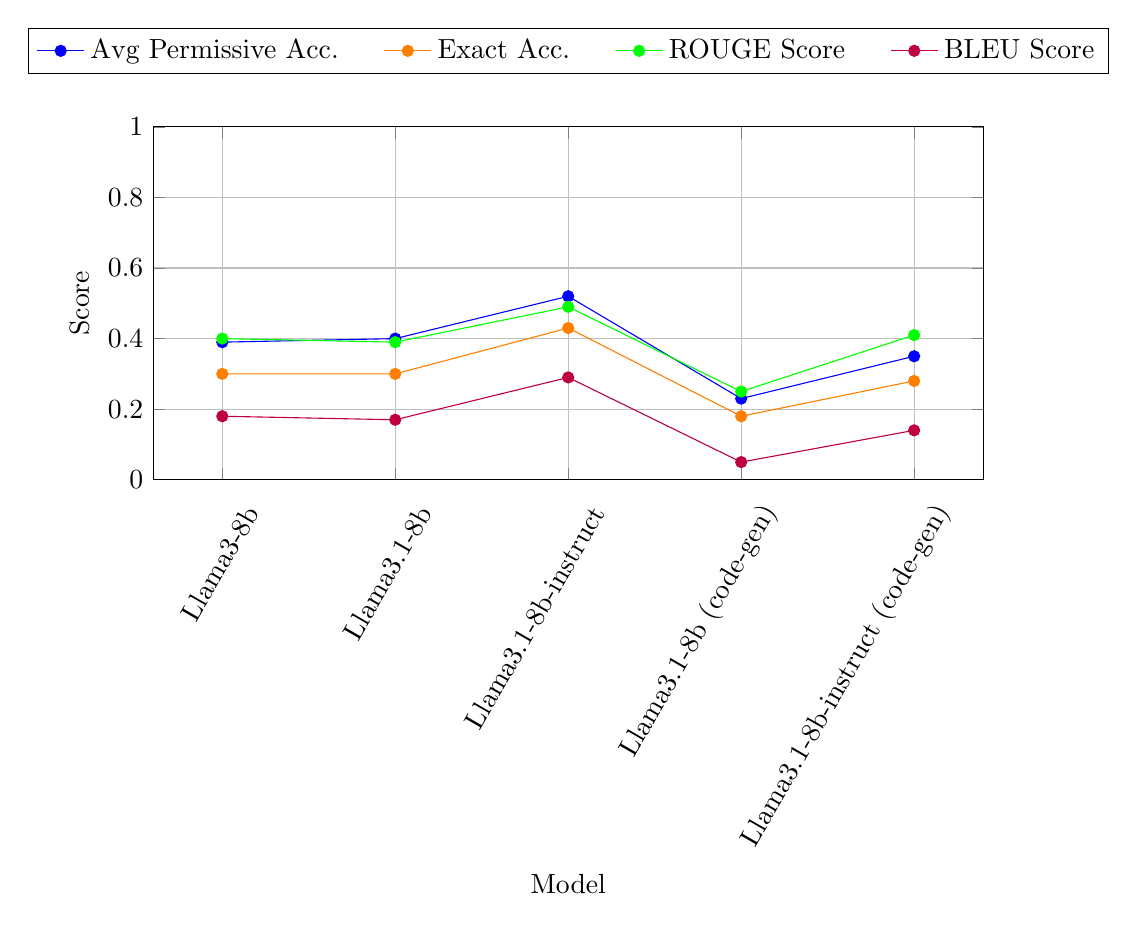
\begin{tikzpicture}
        \begin{axis}[
            width=\textwidth,
            height=0.5\textwidth,
            xlabel={Model},
            ylabel={Score},
            xtick={1,2,3,4,5},
            xticklabels={
                Llama3-8b, 
                Llama3.1-8b, 
                Llama3.1-8b-instruct, 
                Llama3.1-8b (code-gen), 
                Llama3.1-8b-instruct (code-gen)
            },
            xticklabel style={rotate=60, anchor=east, yshift=-0.5cm},
            legend style={at={(0.5,1.15)}, anchor=south,legend columns=-1,/tikz/every even column/.append style={column sep=0.5cm}},
            grid=major,
            ymin=0, ymax=1,
            ]

            % Avg Permissive Acc.
            \addplot[color=blue, mark=*] coordinates {
                (1, 0.39)
                (2, 0.40)
                (3, 0.52)
                (4, 0.23)
                (5, 0.35)
            };
            \addlegendentry{Avg Permissive Acc.}

            % Avg Exact Acc.
            \addplot[color=orange, mark=*] coordinates {
                (1, 0.30)
                (2, 0.30)
                (3, 0.43)
                (4, 0.18)
                (5, 0.28)
            };
            \addlegendentry{Exact Acc.}

            % ROUGE Score
            \addplot[color=green, mark=*] coordinates {
                (1, 0.40)
                (2, 0.39)
                (3, 0.49)
                (4, 0.25)
                (5, 0.41)
            };
            \addlegendentry{ROUGE Score}

            % BLEU Score
            \addplot[color=purple, mark=*] coordinates {
                (1, 0.18)
                (2, 0.17)
                (3, 0.29)
                (4, 0.05)
                (5, 0.14)
            };
            \addlegendentry{BLEU Score}

        \end{axis}
    \end{tikzpicture}
    \caption{Line Plot of Evaluation Metrics for Code Generation | \textcolor{blue}{OMIT This Plot to match the page limit?}}
    \label{fig:metrics-code-line-plot}
\end{figure}
\end{comment}



\begin{comment}
    

\section{Discussion}

Our experiments reveal several important insights into improving number handling capabilities in language models for financial tasks:
\begin{enumerate}
   
 \item \textbf{Model Architecture:} The Llama3-8B architecture demonstrates superior baseline performance compared to Llama2-7B, indicating that newer model iterations have improved inherent number handling abilities.
 \item \textbf{Fine-tuning Effectiveness:} Fine-tuning proves to be a highly effective strategy, significantly boosting performance across all metrics. The fine-tuned Llama3-8B model achieved the best overall results, suggesting that combining advanced architectures with task-specific fine-tuning is a powerful approach. 

 
 \item \textbf{Few-shot Prompting:} While not outperforming fine-tuned models, few-shot prompting strategies show promise, especially when computational resources for full fine-tuning are limited. The similar performance of selective and random few-shot prompting indicates that the quantity of examples may be more crucial than their specific relevance in this domain. Revisiting our research question from Section 5.1 regarding the optimal number and type of examples for few-shot prompting, our initial aim was to use at least five examples from a curated set of 20 diverse samples. However, we encountered two significant constraints that shaped our experimental design. Firstly, the Llama-3-8b model's maximum token length of 8,192 often proved insufficient for prompts with four or five examples. This limitation was particularly challenging for datasets like ConvFinQA (add sample in appendix), which features lengthy input contexts with question-answer history. Truncating these samples risked compromising the essential QA-history structure, leading to poor model generalization and increased hallucination. Secondly, GPU memory constraints frequently resulted in out-of-memory errors when increasing the number of examples in the prompt. While our code allows for adjusting the \textsc{K} value (number of examples), experimenting with larger models or those with increased context lengths was beyond our current computational resources. Looking ahead, we could explore models with larger context windows, more powerful computational setups, and dynamic example selection methods (\textbf{you can mention your code setup and idea in appendix}). 
 In conclusion, our findings suggest that the optimal number of examples for few-shot prompting is context-dependent, influenced by the model's token limit, dataset characteristics, and available computational resources. Further investigation with enhanced capabilities will be crucial in uncovering more definitive answers to this complex question.

 \item \textbf{Example Selection:} Our findings indicate that careful curation of examples for few-shot prompting may not consistently yield statistically significant improvements over random selection. We have conducted thorough analyses to identify potential confounding factors in our approach. One hypothesis we considered was the possibility of model overfitting when incorporating relevant examples in the few-shot approach. However, upon examination of the learning curves (see Figure 5.3 \& 5.4), we can conclusively rule out overfitting as a contributing factor to our observations. We propose an alternative hypothesis: the model may have developed an excessive reliance on the structure or content of the provided relevant examples, potentially leading to reduced generalization capacity. The inclusion of highly specific examples might inadvertently constrain the model's generation capabilities, diminishing its flexibility and adaptability to variations in input data.
The marginally superior performance of random examples compared to carefully selected ones could be attributed to the introduction of diversity, which may enhance the model's ability to generalize across varied contexts. This phenomenon is analogous to the benefits of noise injection during training, which can lead to improved generalization in some cases. To further investigate this phenomenon, we conducted experiments using a combination of relevant and random examples to assess whether a balanced approach would yield improved performance. Our results demonstrate comparable outcomes across various type distributions and weights, suggesting that the model's performance remains consistent even with the introduction of diverse example sets. This finding underscores the need for additional experimentation with a larger number of examples, which is currently beyond our computational resources but presents an intriguing avenue for future research. These observations have potential implications for simplifying the implementation of few-shot learning in practical applications. However, further investigation is necessary to validate these findings across different domains and model architectures.

\begin{figure}[htbp]
    \centering
    % First image
    \begin{minipage}{0.32\textwidth} % Adjust the width of each minipage
        \centering
        \includegraphics[width=\linewidth, height=4cm]{mscdiss-skeleton/one_relevant_example.pdf} % Adjust image path as necessary
        \caption{Training curve for fine tuning with one relevant example}
        \label{fig:one-relevant}
    \end{minipage}\hfill % Maintain a small horizontal fill between the images
    % Second image
    \begin{minipage}{0.32\textwidth}
        \centering
        \includegraphics[width=\linewidth, height=4cm]{mscdiss-skeleton/one_random_example.pdf} % Adjust image path as necessary
        \caption{Training curve for fine tuning with one random example}
        \label{fig:one-random}
    \end{minipage}\hfill
    % Third image
    \begin{minipage}{0.32\textwidth}
        \centering
        \includegraphics[width=\linewidth, height=4cm]{mscdiss-skeleton/combined_examples.pdf} % Adjust image path as necessary
        \caption{Training curve for fine tuning with combined, relevant, randomized and baseline type distributions}
        \label{fig:combined-random} % Ensure each label is unique
    \end{minipage}
\end{figure}

 \item \textbf{Tool-based Approaches:} The high performance of the Langchain-based tool on a subset of tasks highlights the potential of combining language models with specialized financial tools for certain applications.
  \item \textbf{Potential of code generation approach:} Despite using models not primarily designed for code generation, we achieved promising results. This suggests that with more specialized models, the performance could be even better.
  \item \textbf{Impact of instruction tuning:} The consistent outperformance of the instruct model demonstrates the value of instruction tuning in improving code generation capabilities and overall task performance.
  \item \textbf{Challenges in code generation:} The high filtration rate and execution errors, especially in the non-instruct model, highlight the challenges in generating reliable, executable code for complex financial calculations.
  \item \textbf{Trade-off between direct output and code generation:} While code generation offers the potential for more precise calculations, our results show that it currently underperforms compared to direct output. This suggests a need for further refinement of the code generation approach.
  \item \textbf{Scalability and resource limitations:} Our experiments were limited to 8b models due to resource constraints. The significant improvement seen with the instruct model suggests that scaling to larger models (e.g., 70b or 405b) could yield even more impressive results, potentially establishing a new state-of-the-art for numerical precision in financial NLP tasks.
\end{enumerate}
% \section{Comparative Analysis}

% \section{Fine-tuning Strategy Optimization}

% \section{Cross-task Generalization}

% \section{Results and Discussion}
\end{comment}
\chapter{Conclusion}
Our research investigates enhancements for open-source language models in financial domain. Despite recent advancements, LLMs like GPT-4o are yet to match human expertise in numerical reasoning within extensive contexts, often struggling with complex instructions involving multiple tasks or noisy, heterogeneous inputs \cite{zhao2024docmathevalevaluatingmathreasoning, he2024can}. Additionally, while these models exhibit impressive in-context learning abilities, they fall short in relation extraction compared to supervised methods, hindered by ineffective demonstration retrieval and limited in-context application \cite{li2024recallretrievereasonbetter}. Our study underscores that significant improvements in the handling of numerical data for financial tasks can be achieved through the deployment of advanced model architectures, targeted fine-tuning, and the strategic use of few-shot prompting (FSP). Notable improvements were observed with the Llama-3-8b FSP+CoT (Zero shot) model, which combined FSP with Chain-of-Thought (CoT) approaches. This model, tested on a merged dataset, demonstrated an approximate 87.8\% increase in permissive accuracy and a substantial 220\% increase in exact match accuracy over the baseline Llama-3-8b model. Interestingly, despite the prevalent view that FSP and CoT typically enhance LLM performance, our findings reveal that these methods did not consistently yield superior results. Instead, the fine-tuned 8b model exhibited better performance in terms of average permissive accuracy, suggesting that the complexity of financial tasks may diminish the effectiveness of adding numerous relevant examples during inference. An unexpected observation from our study was the inefficacy of increasing the number of relevant examples, which in some instances performed similarly to or even worse than randomly selected examples on certain metrics. This finding leads us to hypothesize that in complex tasks, a model that is meticulously trained with tailored instructions may rely more on structured guidance rather than on multiple example prompts. 

The methodology adopted in our research, which focuses on code generation and execution for financial applications, represents a pioneering endeavor in this field. The approach yielded fascinating outcomes, though it confronted numerous obstacles related to managing hybrid datasets and the subsequent generation of code. Notably, while the specialized code-generating model, CodeLlama-7b-Python, is generally recognized for its superior performance in code generation compared to its baseline variants, it proved inadequate for our dataset-specific challenges. Our study leveraged the code generation capabilities inherent in language models to enhance numerical precision in financial tasks, despite challenges with code reliability. By incorporating instruction tuning, our approach achieved a 55\% performance improvement over non-instruct models, with fewer execution errors and better utilization rates. However, the limitations of our methodology become evident when juxtaposed with traditional direct response strategies. However, our findings affirm the viability of this innovative approach. When implemented with an optimally tuned model that minimizes code execution errors, it has the potential to surpass the outcomes of direct response methodologies. 


%Our research demonstrate and discussed several improvements and scopes in how open source language models can be enhanced to deal with complex domain like finance. Although recent LLMs have demonstrated remarkable performance in solving reasoning problems, the level on which these numerical reasoning skills are effective in real-world scenarios particularly in expert domains like finance is still wanting. It has been observed that current best-performing system (i.e., GPT-4o) still significantly lags behind human experts in solving complex numerical reasoning problems grounded in long contexts. \cite{zhao2024docmathevalevaluatingmathreasoning} Also they still struggle with complex instructions, which can be either complex task descriptions that require multiple tasks and constraints, or complex input that contains long context, noise, heterogeneous information and conversational format \cite{he2024can}. Extracting relation from inputs is another notable issue where although large language models (LLMs) have demonstrated impressive in-context learning (ICL) abilities in various tasks, they still suffer from poor performances compared to most supervised fine-tuned RE methods. Utilizing ICL for RE with LLMs encounters two challenges: (1) retrieving good demonstrations from training examples, and (2) enabling LLMs exhibit strong ICL abilities in Relation extraction \cite{li2024recallretrievereasonbetter}. In conclusion, our research demonstrates that significant improvements in number handling capabilities for financial tasks can be achieved through a combination of advanced model architectures (higher parameters model), fine-tuning, and strategic use of few-shot prompting. We observed some noted improvements by employing combination of FSP and CoT to the 8b model on the merged dataset though the 8b fine tuned model performed better in terms of average permissive accuracy highlighting an interesting observation that although based on general understanding that FSP and CoT approaches significantly improve performance in LLMs on downstream tasks, it is not the case here as the model doesn't perform outstandingly well by incorporating these approaches. Another surprisingly unexpected observation is the inefficacy of adding more number of relevant example on the overall outcome which performed similar or even worse than random on a few metrics. We can conclude with the hypothesis that including approaches known to enhance the performance like FSP, CoT might not be reliable and sufficient in tasks where we deal with hybrid data. The observation we made is that for complex tasks, if the model is trained properly with instruction tuning it, it rely more on it rather than the few shot examples and forcing it to produce step by step results - it can be reiterated that complexity of the task outshine the benefits provided by relevant examples during inference. Though we must acknowledge the limitation of our work where we could provide the model a maximum of 2 examples at random (0,1 or 2) due to compuational resource constraint, but if we can test it on 4-5 examples maybe the results would be different potentially due to added weightage of more samples could guide the model effectively - this would be a question we would like to address in the future work. 




%In conclusion, our research demonstrates that significant improvements in number handling capabilities for financial tasks can be achieved through a combination of advanced model architectures, fine-tuning, and strategic use of few-shot prompting. While fine-tuning provides the best overall performance, few-shot prompting offers a computationally lighter alternative with competitive results.

%Future work should explore the integration of language models with specialized financial tools, as well as investigate the scalability of these approaches to larger and more diverse financial datasets. Additionally, further research into the optimal balance between example relevance and quantity in few-shot prompting could yield valuable insights for practical applications in the financial domain.

%Our novel approach of leveraging code generation capabilities in language models shows promise for improving numerical precision in financial tasks. While challenges remain, particularly in the reliability of generated code, the significant improvements seen with instruction tuning and the potential for scaling to larger models suggest this could be a fruitful direction for future research.
%Future work should focus on:

%Experimenting with larger, more specialized models for code generation.
%Refining the few-shot prompting technique to improve code generation reliability.
%Developing more robust error handling and code execution pipelines.
%Extending this approach to other domains requiring high numerical precision.

%By addressing these areas, we believe this approach could potentially set a new standard for numerical accuracy in NLP tasks across various domains.

%\section{Limitations}

\section{Future Work}

Although our study was limited by computational resources, allowing us to test with a maximum of two examples per prompt due to constraints, future work could explore whether increasing this number to four or five might alter the outcomes. Such investigations could potentially demonstrate that a greater volume of contextual data might more effectively steer model performance. This prospective area of research will aim to further dissect the nuanced applications of LLMs in specialized domains, where the intricate nature of tasks could overshadow the traditional benefits of model enhancements. Future research emerging from our initial investigations holds the potential to profoundly impact code generation and execution in numerically demanding domains. A significant aspect of this future work is the advancement and implementation of larger, domain-specific models tailored to meet the distinct demands of sectors such as finance or related fields. This would involve refining few-shot prompting techniques to bolster code generation reliability, potentially incorporating adaptive prompting mechanisms that evolve through feedback loops, as exemplified by the \textsc{Guided Evolution} framework. This framework uses Large Language Models (LLMs) to supervise mutations and optimize code evolution, reflecting a new direction in model adaptability \cite{10.1145/3638529.3654178}. 

%Furthermore, establishing robust error handling and sophisticated code execution pipelines is crucial for ensuring the practical viability of generated code under variable conditions. Broadening these methodologies to other precision-sensitive fields such as health informatics or quantum computing could reveal new challenges and applications. Moreover, the integration of AI with simulation technologies could facilitate the predictive modeling of code outcomes, providing a virtual testing ground before real-world deployment. Such comprehensive advancements could revolutionize the efficacy and reliability of automated code generation across diverse applications.

% \section{Final Reminder}

% The body of your dissertation, before the references and any appendices,
% \emph{must} finish by page~40. The introduction, after preliminary material,
% should have started on page~1.

% You may not change the dissertation format (e.g., reduce the font size, change
% the margins, or reduce the line spacing from the default 1.5 spacing). Be
% careful if you copy-paste packages into your document preamble from elsewhere.
% Some \LaTeX{} packages, such as \texttt{fullpage} or \texttt{savetrees}, change
% the margins of your document. Do not include them!

% Over-length or incorrectly-formatted dissertations will not be accepted and you
% would have to modify your dissertation and resubmit. You cannot assume we will
% check your submission before the final deadline and if it requires resubmission
% after the deadline to conform to the page and style requirements you will be
% subject to the usual late penalties based on your final submission time.

\bibliographystyle{plain}
\bibliography{mybibfile}
% You may delete everything from \appendix up to \end{document} if you don't need it.
\appendix

\chapter{}

\section{Prompt Templates}
\label{sec:Prompt template-combined}

\begin{tcolorbox}[
    breakable,
    enhanced,
    colback=blue!5!white,
    colframe=white!75!black,
    width=\textwidth,
    boxrule=0.5mm,
    left=2pt,
    right=2pt,
    top=2pt,
    bottom=2pt,
    title=LLAMA2-7B-CHAT-HF Prompt,
    fonttitle=\bfseries\small,
    coltitle=black,
    toptitle=1mm,
    bottomtitle=1mm
]
\begin{lstlisting}[language={}, basicstyle=\ttfamily\small, breaklines=true, breakatwhitespace=true]
<s>[INST]
<<SYS>>
{system_prompt}
<</SYS>>
{user_message} [/INST]
\end{lstlisting}

\small
\textbf{System Prompt:} "You are a helpful AI assistant specializing in financial analysis. Answer the following question based on the given context."
\end{tcolorbox}

\begin{tcolorbox}[
    breakable,
    enhanced,
    colback=blue!5!white,
    colframe=white!75!black,
    width=\textwidth,
    boxrule=0.5mm,
    left=2pt,
    right=2pt,
    top=2pt,
    bottom=2pt,
    title=LLAMA3-8B Prompt,
    fonttitle=\bfseries\small,
    coltitle=black,
    toptitle=1mm,
    bottomtitle=1mm
]
\begin{lstlisting}[language={}, basicstyle=\ttfamily\small, breaklines=true, breakatwhitespace=true]
Below is an instruction that describes a task, 
paired with an input that provides further context. 
Write a response that appropriately completes the request.
### Instruction:
{}
### Input:
{}
### Response:
{}
\end{lstlisting}
\end{tcolorbox}

\begin{tcolorbox}[
    breakable,
    enhanced,
    colback=blue!5!white,
    colframe=white!75!black,
    width=\textwidth,
    boxrule=0.5mm,
    left=2pt,
    right=2pt,
    top=2pt,
    bottom=2pt,
    title=LLAMA3-8B WITH FSP+CoT Prompt,
    fonttitle=\bfseries\small,
    coltitle=black,
    toptitle=1mm,
    bottomtitle=1mm
]
\begin{lstlisting}[
    language={},
    basicstyle=\ttfamily\small,
    breaklines=true,
    breakatwhitespace=true,
    columns=flexible,
    keepspaces=true
]
You are a financial expert assistant. Answer the following question 
based on the given context. It is CRUCIAL that you use 
step-by-step reasoning and provide detailed numerical calculations where applicable. 
Break down your answer into clear, numbered steps. 
If asked to extract subject and object in relation, return only the single 
most relevant and applicable extraction. Use '\n' for line breaks in your response.
Examples:
{examples}
Now, please answer the following question using the same step-by-step 
approach as demonstrated in the Examples:
Context: {context}
Question: {question}
Answer (including calculation steps and final answer, or single 
most relevant relation extraction, use '\n' for line breaks):"""
\end{lstlisting}
\end{tcolorbox}

\begin{tcolorbox}[
    fonttitle=\bfseries\small,
    breakable,
    enhanced,
    colback=blue!5!white,
    colframe=white!75!black,
    width=\textwidth,
    boxrule=0.5mm,
    left=2pt,
    right=2pt,
    top=2pt,
    bottom=2pt,
    title=Improved Few Shot Prompt for Code Generation and Execution,
    fonttitle=\bfseries\small,
    coltitle=black,
    toptitle=1mm,
    bottomtitle=1mm
]

\label{prompt-codegen-python}
\small

Below is an instruction that describes a task, paired with examples and an input that provides further context. Learn from the examples and write a response that appropriately completes the request.

\textbf{### Instruction:} You are an AI assistant specialized in financial analysis. Your task is to generate Python code that answers questions based on given financial data and context. Learn from the examples provided and generate accurate, executable Python code that solves the given problem.

\textbf{Important:} When writing Python code, use actual newline characters to separate lines, not '\\n' string literals. Each line of code should be on its own line in your response.

\textbf{### Examples:} \{examples\}

\textbf{### Input:}
\textbf{Context:} \{context\}
\textbf{### Question:} \{question\}

\textbf{### Response:}
Here's the Python code to answer the question:
\texttt{```python}
\end{tcolorbox}

\section{Samples}
\label{samples}
% Below are some sample examples comparing the model’s predictions to the reference values. The best performing model, highlighted in the table earlier, is used to generate these predictions.
\subsection{TAT-QA Dataset}
\begin{tcolorbox}[colback=blue!5!white, % Light blue background
                 colframe=gray, % Gray frame
                 %title=Sample JSON Data, % Title of the box
                 fonttitle=\bfseries, % Bold font for the title
                 breakable, % Allows the box to break across pages
                 sharp corners, % Sharp corners for the box
                 boxsep=10pt, % Padding around text
                 left=10pt, % Left padding
                 right=10pt, % Right padding
                 top=10pt, % Top padding
                 bottom=10pt, % Bottom padding
                 enlarge left by=-10mm, % Extend the box into left margin
                 enlarge right by=-10mm] % Extend the box into right margin
\label{tat-qa-app}
\textbf{Context}: Actuarial assumptions The Group\textbackslash u2019s scheme liabilities are measured using the projected unit credit method using the principal actuarial assumptions set out below: Notes: 1 Figures shown represent a weighted average assumption of the individual schemes. 2 The rate of increases in pensions in payment and deferred revaluation are dependent on the rate of inflation.\textbackslash nTable:\textbackslash n \textbackslash t2019 \textbackslash t2018 \textbackslash t2017 \textbackslash nWeighted average actuarial assumptions used at 31 March1:\textbackslash t\textbackslash t\textbackslash t\textbackslash nRate of inflation2 \textbackslash t2.9\textbackslash t2.9 \textbackslash t3.0 \textbackslash nRate of increase in salaries \textbackslash t2.7 \textbackslash t2.7 \textbackslash t2.6 \textbackslash nDiscount rate \textbackslash t2.3 \textbackslash t2.5 \textbackslash t2.6 \\
\textbf{Question 1}: What does the Weighted average actuarial assumptions consist of? \\
\textbf{Answer}: Rate of inflation, Rate of increase in salaries, Discount rate \\
\textbf{Question 2}: How much is the 2019 rate of inflation?  \\
\textbf{Answer}: 2.9
\end{tcolorbox}
\subsection{Relation Extraction Dataset}
\begin{tcolorbox}[colback=blue!5!white, % Light blue background
                 colframe=gray, % Gray frame
                 %title=Sample JSON Data, % Title of the box
                 fonttitle=\bfseries, % Bold font for the title
                 breakable, % Allows the box to break across pages
                 sharp corners, % Sharp corners for the box
                 boxsep=10pt, % Padding around text
                 left=10pt, % Left padding
                 right=10pt, % Right padding
                 top=10pt, % Top padding
                 bottom=10pt, % Bottom padding
                 enlarge left by=-10mm, % Extend the box into left margin
                 enlarge right by=-10mm] % Extend the box into right margin
\textbf{Context}: LUXEMBOURG, July 9 National parliaments should be convinced to vote in favour of helping Greece if European leaders can reach a good agreement on Sunday, President of the European Council Donald Tusk said, adding that a deal on debt should be part of the agreement. \\
\textbf{Question }: Given the input sentence, please extract the subject and object containing a certain relation. Relations include: product/material produced; manufacturer; distributed by; industry; position held; original broadcaster; owned by; founded by; distribution format; headquarters location; stock exchange; currency; parent organization; chief executive officer; director/manager; owner of; operator; member of; employer; chairperson; platform; subsidiary; legal form; publisher; developer; brand; business division; location of formation; creator. \\
\textbf{Answer}: position\_held: Donald Tusk, President of the European Council
\end{tcolorbox}
\subsection{ConvFinQA Dataset}
\begin{tcolorbox}[
    colback=blue!5!white, % Light blue background
    colframe=gray, % Gray frame
    fonttitle=\bfseries, % Bold font for the title
    breakable, % Allows the box to break across pages
    sharp corners, % Sharp corners for the box
    boxsep=10pt, % Padding around text
    left=10pt, % Left padding
    right=10pt, % Right padding
    top=10pt, % Top padding
    bottom=10pt % Bottom padding
]
\textbf{Note:} This sample is summarized for clarity and ease of interpretation.\\
In fiscal 2008, revenues in the credit union systems and services business segment increased by 14\% from fiscal 2007. All revenue components within the segment experienced growth. The largest dollar growth was noted in license revenues from Episys AE, our flagship core processing system aimed at larger credit unions, which experienced strong sales throughout the year. Support and service revenue, the largest component of total revenues for the credit union segment, experienced 34\% growth in EFT support and 10\% growth in in-house support. Gross profit in this business segment increased by \$9344 in fiscal 2008 compared to fiscal 2007, due primarily to the increase in license revenue, which carries the highest margins.
liquidity and capital resources we have historically generated positive cash flow from operations and have generally used funds generated from operations and short-term borrowings on our revolving credit facility to meet capital requirements . we expect this trend to continue in the future . the company 2019s cash and cash equivalents increased to \$ 118251 at june 30 , 2009 from \$ 65565 at june 30 , 2008 . the following table summarizes net cash from operating activities (NCOA) in the statement of cash flows: \\
\begin{tabular}{cccc}
\toprule
\textbf{Year} & \textbf{Net Income (\$)} & \textbf{Non-Cash Expenses (\$)} & \textbf{NCOA(\$)} \\
\midrule
2009 & 104681 & 56348 & 206588 \\
2008 & 104222 & 70420 & 181001 \\
2007 & 103102 & 74397 & 174247 \\
\bottomrule
\end{tabular} \\
In 2009, cash used in investing activities was \$59227, including \$3027 in contingent consideration paid on prior years' acquisitions. Capital expenditures were \$31562, compared to \$31105 in 2008. Net cash used in financing activities was \$94675, including the repurchase of shares and payment of dividends. Question: What is the net cash from operating activities in 2009? Answer: 206,588 \\
\textbf{Question:} what about in 2008? \\
\textbf{Answer:} 181001.0
\end{tcolorbox}

\subsection{FinQA Dataset}
\begin{tcolorbox}[
    colback=blue!5!white, % Light blue background
    colframe=gray, % Gray frame
    fonttitle=\bfseries, % Bold font for the title
    breakable, % Allows the box to break across pages
    sharp corners, % Sharp corners for the box
    boxsep=10pt, % Padding around text
    left=10pt, % Left padding
    right=10pt, % Right padding
    top=10pt, % Top padding
    bottom=10pt % Bottom padding
]
\textbf{Note:} This sample is summarized for clarity and ease of interpretation. \\
\textbf{Financial Instruments and Risk Management Summary:}

\textbf{Contingent Liabilities:}
Adjustments for contingent liabilities related to business acquisitions are made until they are settled.

\textbf{Derivatives and Hedging:}
The company utilizes interest rate swaps to hedge its variable rate debts, treating them as cash flow hedges in compliance with FASB ASC Topic 815. These derivatives are effectively managing interest rate risks without affecting earnings, maintaining strict policies against speculative use. Foreign exchange risks are mitigated through forward contracts, notably against the INR, to stabilize operational outcomes against currency fluctuations.

\textbf{Trade Receivables:}
As of the end of 2016 and 2015, the company reported net trade receivables of \$1,639 million and \$1,731 million, respectively. These figures account for allowances for doubtful accounts and adjustments made annually.

\textbf{Significant Transactions in 2015-2016:}
The company settled treasury lock hedges with a notional amount of \$1.0 billion in October 2015, relating to a cash settlement payment of \$16 million recorded under comprehensive earnings, with reclassifications to interest expense planned over ten years.

\begin{tabular}{lcc}
\toprule
\textbf{Description} & \textbf{2016 (\$ in mill.)} & \textbf{2015 (\$ in mill.)} \\
\midrule
Billed Trade Receivables & 1452 & 1546 \\
Unbilled Trade Receivables & 228 & 201 \\
Total Trade Receivables & 1680 & 1747 \\
Allowance for Doubtful Accounts & -41 & -16 \\
Net Trade Receivables & 1639 & 1731 \\
\bottomrule
\end{tabular}


\textbf{Question:} what was the percentage change in total trade receivables net from 2015 to 2016? \\
\textbf{Answer:} -5\%
\end{tcolorbox}

\section{Model's Generated Response}

\subsection{Fine-tuned Llama-3-8b Model}

\subsubsection{Example 1}
\textbf{Context:} AMERICAN TOWER CORPORATION AND SUBSIDIARIES NOTES TO CONSOLIDATED FINANCIAL STATEMENTS (Tabular amou ...
\\
\textbf{Question:} What were note receivables in 2019?
\\
\textbf{Generated output:} 1.1 million
\\
\textbf{Reference:} 1.1
\\
\textbf{Permissive Accuracy:} 1
\\
\textbf{Exact Match Accuracy:} 1

\subsubsection{Example 2}
\textbf{Context:} SUMMARY STATEMENTS OF FINANCIAL POSITION Note: (1) 'Currency translation reserve' relates mainly to ...
\\
\textbf{Question:} What is the average share capital across the 2 years?
\\
\textbf{Generated output:} 4275.5
\\
\textbf{Reference:} 4127
\\
\textbf{Permissive Accuracy:} 0
\\
\textbf{Exact Match Accuracy:} 0

\subsubsection{Example 3}
\label{rel-extraction-sample}
\textbf{Context:} In December 2014, investors who had purchased American Depository Shares (ADSs) of Petrobras on the ...
\\
\textbf{Question:} Given the input sentence, please extract the subject and object containing a certain relation in the sentence according to the following relation types, in the format of "relation1: word1, word2; relation2: word3, word4". Relations include: product/material produced; manufacturer; distributed by; industry; position held; original broadcaster; owned by; founded by; distribution format; headquarters location; stock exchange; currency; parent organization; chief executive officer; director/manager; owner of; operator; member of; employer; chairperson; platform; subsidiary; legal form; publisher; developer; brand; business division; location of formation; creator.
\\
\textbf{Generated output:} stock\_exchange: Petrobras, New York Stock Exchange; headquarters\_location: Petrobras, New York City; location\_of\_formation: Petrobras, Brazil; currency: Petrobras, Brazilian real; stock\_exchange: Petrobras, Brazilian Stock Exchange; headquarters\_location: Petrobras, Rio de Janeiro; location\_of\_formation: Petrobras, Brazil; currency: Petrobras, Brazilian real; stock\_exchange: Petrobras, New York Stock Exchange; headquarters\_location: Petrobras, Rio de Janeiro; location\_of
\\
\textbf{Reference:} stock\_exchange: Petrobras, New York Stock Exchange
\\
\textbf{Permissive Accuracy:} 1
\\
\textbf{Exact Match Accuracy:} 0

\subsection{Llama-3-8b Model with FSP+CoT}
\textit{Note: This example demonstrates the Few-Shot Prompting (FSP) with Chain of Thought (CoT) approach. The context and step-by-step reasoning are shown to illustrate how the model processes information and arrives at an answer.}
\\
\subsubsection{Example: 1}
\label{convfinqa-sample-response}
\textbf{Generated Output:} You are a financial expert assistant. Answer the following question based on the given context. Use step-by-step reasoning and provide numerical calculations where applicable. If asked to extract subject and object in relation, return only the single most relevant and applicable extraction. Use '
' for line breaks in your response.

Examples:
Example 1: [Truncated for brevity] entergy texas, inc. and subsidiaries management 2019s financial discussion and analysis results of operations ... Table: amount ( in millions ) 2016 net revenue \$ 644.2 net wholesale revenue -35.1 ( 35.1 ) purchased power capacity -5.9 ( 5.9 ) transmission revenue -5.4 ( 5.4 ) reserve equalization 5.6 retail electric price 19.0 other 4.4 2017 net revenue \$ 626.8

what percent did net revenue decrease between 2016 and 2017?

Answer:  Calculation:
1. 2016 net revenue: \$644.2 million
2. 2017 net revenue: \$626.8 million
3. Decrease = \$644.2 million - \$626.8 million = \$17.4 million
4. Percent decrease = (\$17.4 million / \$644.2 million) * 100 = 2.7\%
Answer: 2.7\%
Now, please answer the following:
\\
\textbf{Actual Context:} SUMMARY STATEMENTS OF FINANCIAL POSITION Note: (1) 'Currency translation reserve' relates mainly ...
\\
\textbf{Actual Question:} What is the average share capital across the 2 years?

Answer (including calculation steps and final answer, or single most relevant relation extraction, use '
' for line breaks): 4127.5 
\\
\textbf{Reference:} 4127
\\
\textbf{Permissive Accuracy:} 0
\\
\textbf{Exact Match Accuracy:} 0

\subsubsection{Example 2}
\textbf{Context:} AMERICAN TOWER CORPORATION AND SUBSIDIARIES NOTES TO CONSOLIDATED FINANCIAL STATEMENTS (Tabular amou ...
\\
\textbf{Question:} What were note receivables in 2019?
\\
\textbf{Generated output:} 1.1
\\
\textbf{Reference:} 1.1
\\
\textbf{Permissive Accuracy:} 1
\\
\textbf{Exact Match Accuracy:} 1

\subsubsection{Example 3}
\textbf{Context:} Slide 25 demonstrates how our Banquet, Healthy Choice and Marie Callender's brands are leading froze ...
\\
\textbf{Question:} Given phrases that describe the relationship between two words/phrases as options, extract the word/phrase pair and the corresponding lexical relationship between them from the input text. The output format should be "relation1: word1, word2; relation2: word3, word4". Options: product/material produced, manufacturer, distributed by, industry, position held, original broadcaster, owned by, founded by, distribution format, headquarters location, stock exchange, currency, parent organization, chief executive officer, director/manager, owner of, operator, member of, employer, chairperson, platform, subsidiary, legal form, publisher, developer, brand, business division, location of formation, creator.
\\
\textbf{Generated output:} industry: Marie Callender's, food; product\_or\_material\_produced: Marie Callender's, frozen food; owned\_by: Marie Callender's, Conagra Brands; parent\_organization: Marie Callender's, Conagra Brands; subsidiary: Conagra Brands, Marie Callender's; owned\_by: Banquet, Conagra Brands; parent\_organization: Banquet, Conagra Brands; subsidiary: Conagra Brands, Banquet; owned\_by: Healthy Choice, Conagra Brands; parent\_organization:
\\
\textbf{Reference:} distribution\_format: frozen, single
\\
\textbf{Permissive Accuracy:} 0
\\
\textbf{Exact Match Accuracy:} 0

\lstset{
  breaklines=true,
  %postbreak=\mbox{\textcolor{red}{$\hookrightarrow$}\space},
  basicstyle=\ttfamily\small,
  columns=flexible,
  keepspaces=true
}

\subsection{Tool-based Sample}
\textbf{Context:} Cloud \& Cognitive Software * Recast to reflect segment changes. ** 2019 results were impacted by Red...
\\
\textbf{Question:} What percentage of Cloud \& Cognitive Software external revenue was Transaction Processing Platforms in 2019?
\\
\textbf{Code:}
\begin{lstlisting}[language=json]
transaction_processing_platforms_revenue_2019 = 7936
cloud_cognitive_software_revenue_2019 = 23200
percentage_transaction_processing_platforms_2019 = (
    transaction_processing_platforms_revenue_2019 / 
    cloud_cognitive_software_revenue_2019
) * 100
print(f'Percentage of Cloud & Cognitive Software external revenue '
      f'that was Transaction Processing Platforms in 2019: '
      f'{percentage_transaction_processing_platforms_2019:.2f}%')
\end{lstlisting}
\\
\textbf{Prediction:} Percentage of Cloud \& Cognitive Software external revenue that was Transaction Processing Platforms in 2019: 34.21\%
\\
\textbf{Reference:} 34.21
\\
\textbf{Exact Match Accuracy:} 1

\subsection{Llama-3-8b-instruct (Code gen)}
\label{sample-output-code-gen}

\textbf{Context:} Operational performance A Leasing activity We agreed 205 long-term leases in 2019, amounting to £26 million annual rent ...
\\
\textbf{Question:} What is the percentage change in the number of opened or refitted unites in the centres from 2018 to 2019?
\\
\textbf{Generated Code:}
 \begin{lstlisting}[language=json]
{
    "number_of_opened_units_2018 = 262\n
    number_of_opened_units_2019 = 256\n
    difference_in_opened_units = abs(number_of_opened_units_2019 - number_of_opened_units_2018)\n
    percentage_change = (difference_in_opened_units / number_of_opened_units_2018) * 100\n
    print(percentage_change)"
}
\end{lstlisting}
\\
\textbf{Final answer after execution:} -2.2900763358778624
\\
\textbf{Reference:} -2.29
\\
\textbf{Permissive Accuracy:} 1
\\
\textbf{Exact Match Accuracy:} 0

\section{Plots and Metrics}
\subsection{Bar Plot for Code Gen}
\begin{figure}[htbp]
\centering
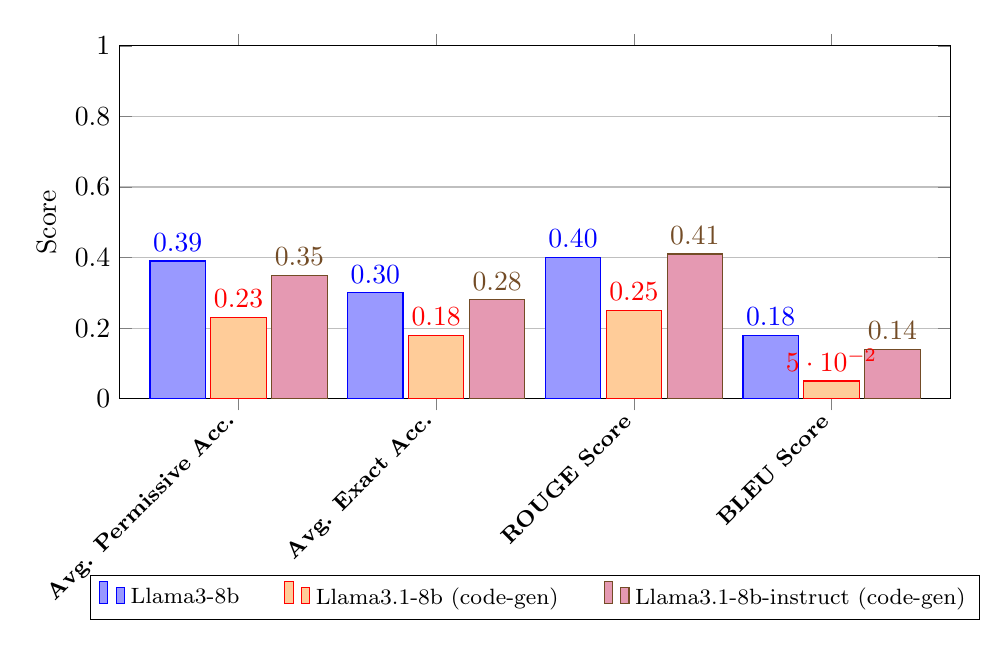
\begin{tikzpicture}
\begin{axis}[
    width=1.0\textwidth,
    height=0.50\textwidth,
    ybar=2pt,
    bar width=20pt,
    ylabel={Score},
    enlarge x limits=0.2,
    symbolic x coords={Avg. Permissive Acc., Avg. Exact Acc., ROUGE Score, BLEU Score},
    xtick=data,
    xticklabel style={rotate=45, anchor=east, font=\footnotesize\bfseries},
    legend style={at={(0.5,-0.5)},
        anchor=north, legend columns=-1,
        font=\footnotesize,
        /tikz/every even column/.append style={column sep=0.5cm}},
    ylabel near ticks,
    ymin=0, ymax=1,
    ymajorgrids,
    nodes near coords={\pgfmathprintnumber[fixed zerofill, precision=2]{\pgfplotspointmeta}},
]
\addplot+[ybar, fill=blue!40] coordinates {
    (Avg. Permissive Acc., 0.39) (Avg. Exact Acc., 0.30) (ROUGE Score, 0.40) (BLEU Score, 0.18)
};
\addplot+[ybar, fill=orange!40] coordinates {
    (Avg. Permissive Acc., 0.23) (Avg. Exact Acc., 0.18) (ROUGE Score, 0.25) (BLEU Score, 0.05)
};
\addplot+[ybar, fill=purple!40] coordinates {
    (Avg. Permissive Acc., 0.35) (Avg. Exact Acc., 0.28) (ROUGE Score, 0.41) (BLEU Score, 0.14)
};
\legend{Llama3-8b, Llama3.1-8b (code-gen), Llama3.1-8b-instruct (code-gen)}
\end{axis}
\end{tikzpicture}
\caption{Evaluation Metrics for Code Generation compared with the base model}
\label{fig:metrics-code-bar-plot}
\end{figure}


\subsection{Training Metrics}

\begin{figure}[H]
    \centering
    % First figure
    \begin{minipage}[b]{0.32\textwidth}
        \centering
        \includegraphics[width=\linewidth,height=4cm,keepaspectratio]{mscdiss-skeleton/one_random_example.pdf}
        \caption{Training Curve for One Random Example}
        \label{fig:random-example}
    \end{minipage}
    \hfill % space between the figures
    % Second figure
    \begin{minipage}[b]{0.32\textwidth}
        \centering
        \includegraphics[width=\linewidth,height=4cm,keepaspectratio]{mscdiss-skeleton/one_relevant_example.pdf}
        \caption{Training Curve for One Relevant Example}
        \label{fig:relevant-example}
    \end{minipage}
    \hfill % space between the figures
    % Third figure
    \begin{minipage}[b]{0.32\textwidth}
        \centering
        \includegraphics[width=\linewidth,height=4cm,keepaspectratio]{mscdiss-skeleton/combined_examples.pdf}
        \caption{Training Curve for Mixed Type Examples}
        \label{fig:mixed-examples}
    \end{minipage}
\end{figure}



% Any appendices, including any required ethics information, should be included
% after the references.

% Markers do not have to consider appendices. Make sure that your contributions
% are made clear in the main body of the dissertation (within the page limit).

% \chapter{Participants' information sheet}

% If you had human participants, include key information that they were given in
% an appendix, and point to it from the ethics declaration.

% \chapter{Participants' consent form}

% If you had human participants, include information about how consent was
% gathered in an appendix, and point to it from the ethics declaration.


\end{document}
